\documentclass[degree=master]{thuthesis}
    % 选项:
    %   degree=[bachelor|master|doctor|postdoctor], % 必选
    %   secret,                                     % 可选
    %   pifootnote,                                 % 可选(建议打开)
    %   openany|openright,                          % 可选,基本不用
    %   arial,                                      % 可选,基本不用
    %   arialtoc,                                   % 可选,基本不用
    %   arialtitle                                  % 可选,基本不用
    
    % 所有其它可能用到的包都统一放到这里了,可以根据自己的实际添加或者删除。
    \usepackage{thuthesis}
    \usepackage{enumerate}
    \usepackage[noend]{algpseudocode}
    \usepackage{algorithmicx,algorithm}
    \renewcommand{\thealgorithm}{\arabic{chapter}.\arabic{algorithm}}
    \floatname{algorithm}{算法}
    \renewcommand{\algorithmicrequire}{ \textbf{输入:}} %Use Input in the format of Algorithm  
    \renewcommand{\algorithmicensure}{ \textbf{输出:}} %UseOutput in the format of Algorithm  

    
    % 定义所有的图片文件在 figures 子目录下
    \graphicspath{{figures/}}
    
    % 可以在这里修改配置文件中的定义。导言区可以使用中文。
    % \def\myname{薛瑞尼}
    
    \begin{document}
    
    %%% 封面部分
    \frontmatter
    \thusetup{
  %******************************
  % 注意:
  %   1. 配置里面不要出现空行
  %   2. 不需要的配置信息可以删除
  %******************************
  %
  %=====
  % 秘级
  %=====
  secretlevel={秘密},
  secretyear={10},
  %
  %=========
  % 中文信息
  %=========
  ctitle={语音情感识别中特征学习和选择的研究},
  cdegree={工程硕士},
  cdepartment={计算机科学与技术系},
  cmajor={计算机技术},
  cauthor={马习},
  csupervisor={贾珈\hspace*{24pt}副教授},
  % csupervisor={吴志勇\hspace*{24pt}副研究员},
  % % cassosupervisor={陈文光教授}, % 副指导老师
  % % ccosupervisor={某某某教授}, % 联合指导老师
  % % 日期自动使用当前时间,若需指定按如下方式修改:
  % % cdate={超新星纪元},
  % %
  % % 博士后专有部分
  % cfirstdiscipline={计算机科学与技术},
  % cseconddiscipline={系统结构},
  % postdoctordate={2009年7月——2011年7月},
  % id={编号}, % 可以留空: id={},
  % udc={UDC}, % 可以留空
  % catalognumber={分类号}, % 可以留空
  %
  %=========
  % 英文信息
  %=========
  etitle={Feature Learning and Selection for Speech Emotion Recognition},
  % 这块比较复杂,需要分情况讨论:
  % 1. 学术型硕士
  %    edegree:必须为Master of Arts或Master of Science(注意大小写)
  %             “哲学、文学、历史学、法学、教育学、艺术学门类,公共管理学科
  %              填写Master of Arts,其它填写Master of Science”
  %    emajor:“获得一级学科授权的学科填写一级学科名称,其它填写二级学科名称”
  % 2. 专业型硕士
  %    edegree:“填写专业学位英文名称全称”
  %    emajor:“工程硕士填写工程领域,其它专业学位不填写此项”
  % 3. 学术型博士
  %    edegree:Doctor of Philosophy(注意大小写)
  %    emajor:“获得一级学科授权的学科填写一级学科名称,其它填写二级学科名称”
  % 4. 专业型博士
  %    edegree:“填写专业学位英文名称全称”
  %    emajor:不填写此项
  edegree={Master of Engineering},
  emajor={Computer Technology},
  eauthor={Ma Xi},
  esupervisor={Associate Professor Jia Jia},
  % esupervisor={Associate Professor Wu Zhiyong},
  % eassosupervisor={Chen Wenguang},
  % 日期自动生成,若需指定按如下方式修改:
  % edate={December, 2005}
  %
  % 关键词用“英文逗号”分割
  % ckeywords={\TeX, \LaTeX, CJK, 模板, 论文},
  % ekeywords={\TeX, \LaTeX, CJK, template, thesis}
}

% 定义中英文摘要和关键字
\begin{cabstract}
  在人机交互日益普遍的今天,只是理解语音中的语言学信息已经不足以满足所有需求,如何提取语音中的情感信息在许多的应用场景中变得越来越重要。但是如何为不同情感更有效地抽取和选择特征并没有被现有的研究广泛关注。针对这个问题,本文分别从传统的语音情感识别方法和端到端的深度学习方法入手,设计对应的方法来抽取和选择特征,以提升系统的情感识别准确率。主要的研究工作和和贡献如下:

  % 传统的语音情感识别大致可以分为情感相关声学特征的提取和情感分类模型的构建两部分,原始语音信号通常会先被映射到情感信息相关的声学特征,然后采用各种分类模型将特征向量映射到对应的情感类别。近年来,随着深度学习方法的发展与普及,深度神经网络开始越来越多被应用到语音情感识别,并且取得了不错的效果。此外,特征提取和情感分类两个部分也开始被整合到一起,通过深度神经网络将可以构建从原始语音信号直接到情感类别的端到端的识别系统,
 
\textbf{一、提出了一种基于情感对的语音情感识别框架,为不同的情感对选择不同的声学特征,并在最后的决策融合过程中引入心理学的情感空间模型,提升系统的识别准确率。} 传统的语音情感识别系统通常为所有的情感选取相同的声学特征来完成最后的情感分类,但实验证明不同的情感和不同的声学特征的相关性并不同。针对这一问题,我们分别为不同的情感对选取不同的特征集合,将原先的多分类问题转变为多个二分类问题,并在最后的决策融合过程中通过贝叶斯分类器引入情感空间的信息。
% 在公开的情感语音数据集IEMOCAP上,我们方法取得了比传统的识别框架更好的准确率。

\textbf{二、构建了基于深度神经网络的端到端的语音情感识别系统,使用语谱图代替传统的声学特征,从而提升情感识别准确率。} 随着深度学习技术和工具的发展,许多的研究者开始采用深度神经网络在原始语音信号上直接构建分类或者回归模型,被称之为端到端的系统。相比于传统的声学特征,这种方法可以抽取到更符合任务目标的特征表示。语谱图是语音信号的一种无损表示,我们通过卷积神经网络从语谱图上直接抽取和情感相关的特征表示,然后通过循环神经网络来建模语音信号的时序信息,最后通过全连接网络将输出映射到不同情感的后验概率。
% 相比于传统的语音情感识别,端到端的系统能够取得更好的准确率。

\textbf{三、设计了一种能够处理变长语音段的神经网络结构来实现端到端的系统,消除了语音分段带来的中性语音和情感语音的混淆,进一步提升了情感识别的准确率。} 在使用深度神经网络实现端到端的语音情感识别系统时,由于模型很难处理变长的输入,通常会把变长的语音句子切分成多个等长的语音段,然后将所有语音段都标记为对应句子的情感标签,但这样会导致部分中性语音段被标记为有情感。针对于这一问题,我们采用补齐和掩码的方式来处理神经网络中变长的输入序列,保证模型可以接受整个语音句子,从而避免了错误标注带来的效果变差。
% 相对于切分等长语音段的方法,我们直接输入整个变长语音句子的方法可以在相同的数据集上取得更好的准确率。
 
\end{cabstract}

% 如果习惯关键字跟在摘要文字后面,可以用直接命令来设置,如下:
\ckeywords{语音情感识别;情感对;维度情感空间模型;端到端深度神经网络;变长语音段}

\begin{eabstract}
  Nowadays human-machine interaction is becoming more and more popular. The machine only understands linguistic information in speech, which is not enough to satisfy all needs. How to extract emotional information in speech is becoming more and more important in many application scenarios. However, how to extract and select features more effectively for different emotions has not been widely studied. In order to solve this problem, this paper will design the corresponding methods to extract and select features with traditional speech emotion recognition and end-to-end speech emotion recognition, and then improve the recognition rate of the system. The main contributions of this paper include:

  % Traditional speech emotion recognition can be divided into two parts: acoustic feature extraction and emotion classification model. The original speech signals are usually mapped to the acoustic features, and then use the classification models to map the features into the corresponding emotional categories. In the recent years, with the development of deep learning, deep neural networks have been introduced to speech emotion recognition, and have achieved good results. Furthermore, feature extraction and emotion classification are beginning to the integrated together. Through deep neural network, the end-to-end recognition system can be builded from original speech signals to emotional categories.

\textbf{1. A emotion-pair based speech emotion recognition framework is proposed to select different features for different emotion-pairs, and the dimensional emotion space is introduced in the decision fusion, thus improving the recognition rate of the system.}  In general, the traditional speech emotion recognition system select the same acoustic features for all emotions to complete the emotion classification, but the studies have shown that the correlation between different emotions and different acoustic features is different. To solve this problem, we will select different acoustic features for different emotions, and turn the multi-classification problem into bi-classification problems. In the decision fusion stage, the information of emotional space is introduced by Bayes classifier. 
% In the IEMOCAP emotional speech dataset, our method can achieve better accuracy than the traditional recognition framework.

\textbf{2. The deep neural network based end-to-end speech emotion recognition system is constructed, which uses the spectrogram instead of the acoustic features, thus improving performance of emotion recognition.}  With the development of deep learning techniques and tools, many researchers have begun to use deep neural network to directly construct classification and regression models on original speech signals, the so-called end-to-end system. Compared with traditional acoustic features, this method can extract feature representations which are more related to the target. Spectrogram is a lossless representation of speech signals. We use the convolution neural networks to extract the emotion related features directly from the spectrogram,  and then model the time sequence information of the speech signals through recurrent neural networks, and the map the output to the posterior probability of the different emotions through the full-connected neural networks. 
% Compared to the traditional speech emotion recognition, the end-to-end system can achieve better accuracy.

\textbf{3. A neural network structure which can handle the variable-length speech segments is designed to implement the end-to-end system. This structure can relieves the confusion between neutral speech and emotional speech brought by the speech segmentation, thus further improving the recognition rate of the system.} When using deep neural networks to implement the end-to-end speech emotion recognition system, because the model is difficult to deal with the variable-length input, the speech sentences are usually divided into multiple equal-length speech segments, and all the speech segments are labeled as the emotional labels of the corresponding sentence. However, this causes some neutral speech segments to be marked with other emotions. In order to solve this problem, we use the method of padding and masking to deal with the variable-length input sequence in the neural networks, and ensure that the model can accept the whole speech sentence. This will avoid the performance degeneration through introducing the wrong labels. 
% Compared with the method of segmenting equal-length speech segments, we can get better accuracy on the same dataset by directly inputting the whole variable-length speech sentence.

\end{eabstract}

\ekeywords{Speech Emotion Recognition; Emotion-Pair; Dimensional Emotion Space; End-to-End Deep Neural Network; Variable-Length Speech Segments}

    % 如果使用授权说明扫描页,将可选参数中指定为扫描得到的 PDF 文件名,例如:
    % \makecover[scan-auth.pdf]
    \makecover
    
    %% 目录
    \tableofcontents
    
    %% 符号对照表
    % \begin{denotation}[3cm]
\item [HMM] 隐马尔科夫模型 (Hidden Markov Model)
\item [GMM] 高斯混合模型 (Gaussian Mixture Model)
\item [SVM] 支持向量机 (Support Vector Machine)
\item [BLR] 贝叶斯逻辑回归 (Bayesian Logistic Regression)
\item [DNN] 深度神经网络 (Deep Neural Network)
\item [CNN] 卷积神经网络 (Convolution Neural Network)
\item [RNN] 循环神经网路 (Recurrent Neural Network)
\item [LSTM] 长短时记忆 (Long-Short Time Memory)
\item [GRU] 门循环单元 (Gated Recurrent Unit)
\item [RBM] 受限玻尔兹曼机 (Restricted Boltzmann Machine)
\item [DBN] 深度信念网络 (Deep Belief Network)
\item [LPC] 线性预测系数 (Linear Prediction Coefficients)
\item [LPCC] 线性预测倒谱系数 (Linear Prediction Cepstral Coefficients)
\item [MFCC] 梅尔频率倒谱系数 (Mel-frequency Cepstral Coefficients)
\item [SFFS] 序列浮动前向选择算法 (Sequential Floating Forward Selection)
\item [PCA] 主成分分析 (Principal Component Analysis)
\item [LDA] 线性判别分析 (Linear Discriminant Analysis)
\item [SVD] 奇异值分解 (Singular Value Decomposition)
\item [GA] 遗传算法 (Genetic Algorithm)
\item [EM] 期望最大化 (Expectation Maximization)
\item [UA] 不加权准确率 (Unweighted Accuracy)
\item [WA] 加权准确率 (Weighted Accuracy)
\item [ELM] 极限学习器 (Extreme Learning Machine)
\item [STFT] 短时傅里叶变换 (Short-Time Fourier Transform)
\end{denotation}

    
    
    %%% 正文部分
    \mainmatter
    \chapter{绪论}
\label{cha:intro}

\section{研究背景和意义}
\label{sec:background}
语音作为人与人之间交流最为自然的一种媒介,在我们的日常生活中起着至关重要的作用,这也使得语音一直被许多研究者认为是最有效的人机交互方式。在最近的二十年间,语音识别技术已经取得飞速的发展,它的目的是将人们说出的语音转换成对应的词序列。尽管语音识别技术已经被广泛的应用,但我们和真正的自然人机交互仍然有很大的距离,因为机器仍然无法理解说话人的情感状态,而语音通常会包含说话人当时的情感状态信息。这使得语音情感识别技术开始受到重视,它的目的就是从语音中抽取说话人的情感状态。

语音情感识别在许多需要自然人机交互的系统特别有用,例如网页影评和计算机辅助教育这些需要用户反馈的应用场景。在车载系统中,情感识别可以通过语音检测驾驶员当前的精神状态,并在合适的时候做出提醒从而保证车辆安全。语音情感识别还可以作为心理咨询师提供诊断的辅助工具。在同声传译系统中,语音情感识别也可以通过检测说话人情感状来调整翻译内容。对于语音识别系统来说,加入情感信息同样可以提高识别准确率。还有在电话客服系统中,客户由于长时间的等待或者紧迫的需求,声音会变的烦躁和愤怒。在这种情况下,情感识别系统就可以通过检测语音中愤怒的程度来为这些客户安排服务优先级。此外,在聊天机器人中,语音情感识别系统可以通过检测对方的情感状态来做出不同的应答。这种功能同样也可以运用在玩具中,当孩子不高心的时候,玩具就可以通过一些方式安抚他们。在电子游戏中,尤其是在一些有语音交互的游戏中,情感识别可以通过模拟更加真实的交互场景来提升游戏体验。因此,语音情感识别在近几年来收到越来越多的关注。无论是在前沿模型算法的研究,还是在相关产品的落地,很多研究机构和公司都在这一领域投入大量的精力。

语音情感识别也存在许多挑战性的问题。首先,很难确定哪些声学特征与情感信息最相关。一些在语音识别领域公认的特征,例如梅尔频率倒谱系数(Mel-Frequency Cepstral Coefficients, MFCC), 在语音情感识别上并没有取得好的效果,其次,一段语音中有时会包含多种情感,如何找到每种情感对应的语音边界是个很有挑战性的问题。此外,由于说话人的文化背景不同,也会导致表达情感的方式不太相同。例如有的人愤怒时会说话很大声,而有的人却声音很低沉。语言也是影响情感表达的一个主要问题。还有就是情感并没有公认的规范定义,只能通过人们的主观感觉来区分,但这会导致有许多的情感类别。许多的研究者都倾向于一种“调色板”理论,就是只定义几种基本的情感,然后其他的情感都是由这些基本情感以不同的比例调和而成,这些基本情感被称为原型情感。情感语音的数据相对来说也很难获取,这会导致许多复杂的模型无法得到充分训练。

尽管目前还没有非常成熟的语音情感识别的产品,但许多公司已经在极力推动这一领域的产品落地。Facebook早在2012年就开始进行对用户的情绪检测实验,期望能够通过情感信息来优化他们的推荐系统。微软小冰也嵌入了语音情感识别模块,希望能够和人们更自然的聊天。IBM与软银合作推出了具有情绪感知能力的机器人Pepper。苹果也开始在自己的产品中加入语音情感识别的功能。国内的公司在近几年也开始这一领域的产品化,科大讯飞公司已经开始推出语音情感识别相关的技术支持,百度视频也推出基于情感识别的内容推荐系统。此外,也有一些创业公司开始关注语音情感识别,例如竹简智能。

\section{研究现状}
\label{sec:status}
语音情感识别根据处理流程不同大致可以分为两种类型,一种是传统从语音信号中抽取声学特征,然后通过分类器区分情感类别,另一种是直接将原始语音信号映射到情感类别的端到端系统,下面将分别介绍这这两类方法。

\subsection{传统的语音情感识别}
\label{ssec:classical_emo_rec}
传统的语音情感识别主要可以分为两个部分,第一部分是抽取和情感信息相关的声学特征,第二部分是使用分类器将特征向量映射到对应的情感类别,图\ref{fig:traditional_speech_emotion_recognition}是传统语音情感识别的流程图。

\begin{figure}[htb] % use float package if you want it here
    \centering
    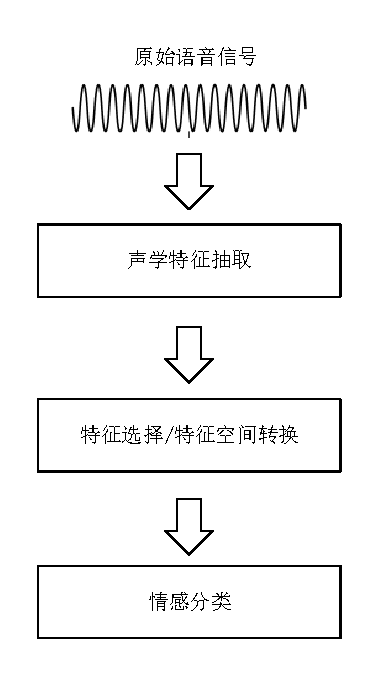
\includegraphics[height=10cm]{myfigures/traditional_speech_emotion_recognition}
    \caption{传统语音情感识别流程图}
    \label{fig:traditional_speech_emotion_recognition}
\end{figure}

特征选择是一个在所有分类问题中都存在的问题,目的是抽取与分类目标最相关的特征子集。语音情感识别作为一个分类任务,在这方面已经有很多的研究工作。首先,韵律学相关的特征已经被广泛的应用在语音情感识别,包括基频相关的特征,能量相关的特征和时长相关的特征。其次,谱相关的特征也在情感识别中起到了重要的作用,例如线性预测系数(Linear Prediction Coefficients, LPC),线性预测倒谱系数(Linear Prediction Cepstral Coefficients, LPCC)以及梅尔频率倒谱系数(Mel-frequency Cepstral Coefficients, MFCC)。此外,声音质量相关的特征也被证明同情感识别任务相关。

从语音信号中抽取声学特征后,接下来就变成了一个基本的分类问题,有许多的分类模型已经被运用在情感识别任务中。隐马尔可夫模型(Hidden Markov Model, HMM)是被广泛使用在语音识别中的一种模型,它的运作原理和语音产生的机制十分相似,因此这种模型同样也在语音情感识别中被使用。高斯混合模型(Gaussian Mixture Models, GMM)是一种概率分布模型,它使用多变量的高斯分布来预测当前语音句子属于不同情感类别的概率,在一些公开数据集上取得了不错的效果。支持向量机(Support Vector Machine, SVM)是一种被广泛使用在许多模式识别任务中的分类模型,它通过核函数(Kernel Functions)将低维空间无法区分的特征向量映射到更高维的空间,然后用线性分类器将其区分,这种模型在许多语音情感识别的研究中也被使用。随着计算能力和存储容量的提升,深度学习模型在近几年变得逐渐流行,在许多的任务上都超过了传统的机器学习算法。在语音情感识别领域,深度学习的方法同样也被广泛使用。除了上面这些单独的分类模型,还有一些工作尝试将多种模型混合使用,然后共同决策最后的情感类别,期望能够提高系统的鲁棒性。

\subsection{端到端的语音情感识别}
\label{ssec:end2end_emo_rec}
在最近几年,深度学习的方法和工具已经被运用到语音处理领域,包括用于特征抽取,分类和回归任务,或者两者兼而有之。一些试验结果显示在原始语音信号上使用深度神经网络提取特征可以比采用人工定义的声学特征得到更好的效果。这导致许多的研究者开始采用端到端的系统,即省略声学特征提取的过程,直接建立从原始语音信号到任务目标的映射,图\ref{fig:end2end_speech_emotion_recognition}是端到端的语音情感识别流程图。

\begin{figure}[htb] % use float package if you want it here
    \centering
    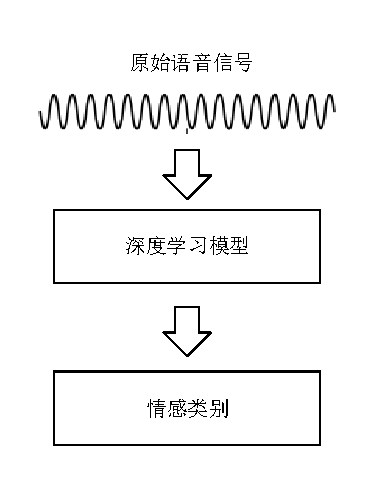
\includegraphics[height=10cm]{myfigures/end2end_speech_emotion_recognition}
    \caption{端到端语音情感识别流程图}
    \label{fig:end2end_speech_emotion_recognition}
\end{figure}

这种端到端的系统最早出现在语音识别领域,最早的工作是Jaitly等人通过受限玻尔兹曼机(Restricted Boltzmann Machine, RBM)从原始语音信号上得到一种有利于语音识别的中间表示。Bhargava等人则是通过堆叠的全连接神经网络从原始语音信号得到瓶颈特征(Bottleneck Feature),并且取得了和使用梅尔频率倒谱系数相近的效果。 Sainath等人将CNN和LSTM-RNN用在大词表语音识别上。Hannun和Amodei在线性语谱图(Linearly-Spaced Spectrogram)上采用深度神经网络,并搭建出了当时最好的语音识别系统。此外,梅尔语谱图(Mel-Scale Spectrogram)上使用深度学习方法,在说话人识别上也取得了很不错的效果

在语音情感识别领域也开始有一些端到端的方法被提出。George等人提出一种使用CNN从原始语音信号提取特征,然后通过LSTM-RNN捕获输入序列的时序信息并最终输出不同情感的后验概率,并且他们发现LSTM-RNN不同节点的输出和一些声学特征有很强的相关性。Satt等人也采用了相似的神经网络结构,但不同的是他们从语谱图(Spectrogram)上抽取特征而非原始语音信号。他们认为在语谱图上可以更方便的进行去噪的操作,并且他们在公开情感语音数据集IEMOCAP上取得了超过之前最好结果(The State of Art)的准确率。

\section{本文的主要研究内容和贡献}
\label{sec:content_contribution}

\subsection{研究内容和各章介绍}
\label{ssec:content}
语音情感识别效果与声学特征的选取是密切相关的,抽取什么特征以及如何抽取特征最终会影响到识别率。本文会从传统的语音情感识别和端到端的语音情感识别两类方法分别研究特征抽取的方法,意使最终的情感识别准确率得到提高。

 第\ref{cha:basic_konwledge}章主要介绍语音情感识别相关的基础知识,包括情感的定义,情感语音数据库,情感相关的声学特征以及情感分类模型这四个方面的内容。首先,我们介绍了两种不同的情感定义方式,并分析了各自的优缺点。接下来我们介绍了不同类型的情感语音数据库,包括他们的采集方式和标注方式。然后我们会对情感相关的声学特征做一个全面的介绍,包括特征类型,特征选择算法和深度神经网络抽取特征。最后我们会对不同的语音情感分类模型做出介绍,包括传统的机器学习模型和深度学习模型。

 第\ref{cha:emo_pair_base_framework}章介绍了基于情感对的语音情感识别框架。通过将任意两种不同的情感组成情感对,并为不同的情感对分别选择不同的特征子集构建二分类器,从而得到更精确的二分类结果。进一步,我们发现在维度情感空间中,不同情感之前的距离并不相同,距离越近表示情感之间更相似,越远表示越不相似。依据这种信息,我们构建贝叶斯分类器来对所有情感对的输出结果做决策融合,从而得到最终的情感类别。在实验结果上我们超过了为所有情感的分类选取相同特征集的方法,同时我们的效果也优于基于决策树的分层识别框架,这种框架的设计思想和我们很相似,但我们的方法效果更好,而且当情感类别变化时更方便构建。

 第\ref{cha:end2end}章介绍了基于深度学习的端到端的情感识别方法。在这一章我们将不再采用传统的声学特征提取方法,而是转而使用深度神经网络将语谱图(Spectrogram)直接映射到对应的情感类别。我们会将语音信号首先转换为语谱图,然后采用CNN直接在语谱图上抽取特征。由于语音信号属于时间序列信号,因此在CNN抽取特征后我们将采用RNN建模输入序列的时序信息,并将最后一个时间步的输出传给后面的全连接网络,最后通过全连接网络将输入映射到每种情感的后验概率。相比于传统声学特征,采用语谱图作为输入可以取得更好的识别效果。
 
 第\ref{cha:var_len}章介绍了如何设计能够处理变长语音段的深度神经网络结构。上一章将句子切分成多个更短的等长语音段,并给将每个语音段都标记为句子所属的情感类别,因为大多数网络结构更容易去处理定长的输入序列,但是将句子切分成更短的等长语音段无法保证每个语音段都包含有情感信息,这会导致网络在训练时对中性语音和情感语音产生混淆。因此,我们设计了一种能够处理变长语音段的神经网络结构,通过掩码可以保证在训练和测试的过程中都不需要对语音段进行切分,这样就可以避免上面的问题。实验结果显示,变长方法在公开的情感语音数据库IEMOCAP上超过了定长方法得到的最好准确率。

 第\ref{cha:summary_prospect}章对本文中关于语音情感识别中声学特征的相关研究成果进行了总结,同时,还对基于情感对的识别框架和基于深度学习的端到端的框架的使用前景进行了展望。

\subsection{本文主要贡献}
\label{ssec:contribution}
本文的主要贡献点有以下几个方面:

\textbf{一、提出一种基于情感对的语音情感识别框架,为不同的情感对选择不同的声学特征,并在最后的决策融合过程中引入心理学的情感空间模型,从而提升了系统的识别率。} 传统的语音情感识别系统通常为所有的情感选取相同的声学特征来完成最后的情感分类,但实验证明不同的情感和不同的声学特征的相关性并不同。针对这一问题,我们将分别为不同的情感对选取不同的特征集合,将原先的多分类问题转变为多个二分类问题,并在最后的决策融合过程中通过贝叶斯分类器引入情感空间的信息。在公开的情感语音数据集IEMOCAP上,我们方法取得了比传统的识别框架更好的准确率。

\textbf{二、构建了基于深度神经网络的端到端的语音情感识别系统,使用语谱图代替传统的声学特征,从而提升了系统的识别率。} 随着深度学习技术和工具的发展,许多的研究者开始采用深度神经网络在原始语音信号上直接构建分类或者回归模型,被称之为端到端的系统。相比于采用传统的声学特征,这种方法可以抽取到更符合任务目标的特征表示。语谱图是语音信号的一种无损表示,我们通过卷积神经网络来从语谱图上直接抽取和情感相关的特征表示,然后通过循环神经网络来建模语音信号的时序信息,最后通过全连接网络将输出映射到不同情感的后验概率。相比于采用传统的声学特征,端到端的系统能够取得更好的准确率。

\textbf{三、设计了一种能够处理变长语音段的神经网络结构来实现端到端的系统,消除了语音分段带来的中性语音和情感语音的混淆,从而提升了系统的识别率。} 在使用深度神经网络实现端到端的语音情感识别系统时,由于卷积神经网络和循环神经网络很难处理变长的输入,通常会把变长的语音句子切分成多段等长的语音段,然后将所有语音段都标记为对应句子的情感标签,但这样会导致部分中性语音段被标记为有情感。针对于这一问题,我们采用补齐和掩码的方式来处理神经网络中变长的输入序列,避免了错误标注带来了的效果变差。相对于切分等长语音段的方法,我们直接输入整个变长语音句子的方法可以在相同的数据集上取得更好的准确率。


% 苏轼(1037-1101),北宋文学家、书画家。字子瞻,号东坡居士,眉州眉山(今属四川)人
% 。苏洵子。嘉佑进士。神宗时曾任祠部员外郎,因反对王安石新法而求外职,任杭州通判,
% 知密州、徐州、湖州。后以作诗“谤讪朝廷”罪贬黄州。哲宗时任翰林学士,曾出知杭州、
% 颖州等,官至礼部尚书。后又贬谪惠州、儋州。北还后第二年病死常州。南宋时追谥文忠。
% 与父洵弟辙,合称“三苏”。在政治上属于旧党,但也有改革弊政的要求。其文汪洋恣肆,
% 明白畅达,为“唐宋八大家”之一。  其诗清新豪健,善用夸张比喻,在艺术表现方面独具
% 风格。少数诗篇也能反映民间疾苦,指责统治者的奢侈骄纵。词开豪放一派,对后代很有影
% 响。《念奴娇·赤壁怀古》、《水调歌头·丙辰中秋》传诵甚广。

% {\kaishu 坡仙擅长行书、楷书,取法李邕、徐浩、颜真卿、杨凝式,而能自创新意。用笔丰腴
%   跌宕,有天真烂漫之趣。与蔡襄、黄庭坚、米芾并称“宋四家”。能画竹,学文同,也喜
%   作枯木怪石。论画主张“神似”,认为“论画以形似,见与儿童邻”;高度评价“诗中有
%   画,画中有诗”的艺术造诣。诗文有《东坡七集》等。存世书迹有《答谢民师论文帖》、
%   《祭黄几道文》、《前赤壁赋》、《黄州寒食诗帖》等。  画迹有《枯木怪石图》、《
%   竹石图》等。}

% {\fangsong 易与天地准,故能弥纶天地之道。仰以观於天文,俯以察於地理,是故知幽明之故。原
%   始反终,故知死生之说。精气为物,游魂为变,是故知鬼神之情状。与天地相似,故不违。
%   知周乎万物,而道济天下,故不过。旁行而不流,乐天知命,故不忧。安土敦乎仁,故
%   能爱。范围天地之化而不过,曲成万物而不遗,通乎昼夜之道而知,故神无方而易无体。}

% % 非本科生一般用不到幼圆与隶书字体。需要的同学请查看 ctex 文档。
% {\ifcsname youyuan\endcsname\youyuan\else[无 \cs{youyuan} 字体。]\fi 有天地,然后
%   万物生焉。盈天地之间者,唯万物,故受之以屯;屯者盈也,屯者物之始生也。物生必蒙,
%   故受之以蒙;蒙者蒙也,物之穉也。物穉不可不养也,故受之以需;需者饮食之道也。饮
%   食必有讼,故受之以讼。讼必有众起,故受之以师;师者众也。众必有所比,故受之以比;
%   比者比也。比必有所畜也,故受之以小畜。物畜然后有礼,故受之以履。}

% {\heiti 履而泰,然后安,故受之以泰;泰者通也。物不可以终通,故受之以否。物不可以终
%   否,故受之以同人。与人同者,物必归焉,故受之以大有。有大者不可以盈,故受之以谦。
%   有大而能谦,必豫,故受之以豫。豫必有随,故受之以随。以喜随人者,必有事,故受
%   之以蛊;蛊者事也。}

% {\ifcsname lishu\endcsname\lishu\else[无 \cs{lishu} 字体。]\fi 有事而后可大,故受
%   之以临;临者大也。物大然后可观,故受之以观。可观而后有所合,故受之以噬嗑;嗑者
%   合也。物不可以苟合而已,故受之以贲;贲者饰也。致饰然后亨,则尽矣,故受之以剥;
%   剥者剥也。物不可以终尽,剥穷上反下,故受之以复。复则不妄矣,故受之以无妄。}

% {\songti 有无妄然后可畜,故受之以大畜。物畜然后可养,故受之以颐;颐者养也。不养则不
%   可动,故受之以大过。物不可以终过,故受之以坎;坎者陷也。陷必有所丽,故受之以
%   离;离者丽也。}

% \section{表格样本}
% \label{chap1:sample:table} 

% \subsection{基本表格}
% \label{sec:basictable}

% 模板中关于表格的宏包有三个:\pkg{booktabs}、\pkg{array} 和 \pkg{longtabular},命
% 令有一个 \cs{hlinewd}。三线表可以用 \pkg{booktabs} 提供
% 的 \cs{toprule}、\cs{midrule} 和 \cs{bottomrule}。它们与 \pkg{longtable} 能很好的
% 配合使用。如果表格比较简单的话可以直接用命令 \cs{hlinewd}\marg{width} 控制。
% \begin{table}[htb]
%   \centering
%   \begin{minipage}[t]{0.8\linewidth} % 如果想在表格中使用脚注,minipage是个不错的办法
%   \caption[模板文件]{模板文件。如果表格的标题很长,那么在表格索引中就会很不美
%     观,所以要像 chapter 那样在前面用中括号写一个简短的标题。这个标题会出现在索
%     引中。}
%   \label{tab:template-files}
%     \begin{tabularx}{\linewidth}{lX}
%       \toprule[1.5pt]
%       {\heiti 文件名} & {\heiti 描述} \\\midrule[1pt]
%       thuthesis.ins & \LaTeX{} 安装文件,\textsc{DocStrip}\footnote{表格中的脚注} \\
%       thuthesis.dtx & 所有的一切都在这里面\footnote{再来一个}。\\
%       thuthesis.cls & 模板类文件。\\
%       thuthesis.cfg & 模板配置文。cls 和 cfg 由前两个文件生成。\\
%       thuthesis-numeric.bst    & 参考文献 BIB\TeX\ 样式文件。\\
%       thuthesis-author-year.bst    & 参考文献 BIB\TeX\ 样式文件。\\
%       thuthesis.sty   & 常用的包和命令写在这里,减轻主文件的负担。\\
%       \bottomrule[1.5pt]
%     \end{tabularx}
%   \end{minipage}
% \end{table}

% 首先来看一个最简单的表格。表 \ref{tab:template-files} 列举了本模板主要文件及其功
% 能。请大家注意三线表中各条线对应的命令。这个例子还展示了如何在表格中正确使用脚注。
% 由于 \LaTeX{} 本身不支持在表格中使用 \cs{footnote},所以我们不得不将表格放在
% 小页中,而且最好将表格的宽度设置为小页的宽度,这样脚注看起来才更美观。

% \subsection{复杂表格}
% \label{sec:complicatedtable}

% 我们经常会在表格下方标注数据来源,或者对表格里面的条目进行解释。前面的脚注是一种
% 不错的方法,如果不喜欢脚注,可以在表格后面写注释,比如表~\ref{tab:tabexamp1}。
% \begin{table}[htbp]
%   \centering
%   \caption{复杂表格示例 1}
%   \label{tab:tabexamp1}
%   \begin{minipage}[t]{0.8\textwidth} 
%     \begin{tabularx}{\linewidth}{|l|X|X|X|X|}
%       \hline
%       \multirow{2}*{\diagbox[width=5em]{x}{y}} & \multicolumn{2}{c|}{First Half} & \multicolumn{2}{c|}{Second Half}\\\cline{2-5}
%       & 1st Qtr &2nd Qtr&3rd Qtr&4th Qtr \\ \hline
%       East$^{*}$ &   20.4&   27.4&   90&     20.4 \\
%       West$^{**}$ &   30.6 &   38.6 &   34.6 &  31.6 \\ \hline
%     \end{tabularx}\\[2pt]
%     \footnotesize 注:数据来源《\thuthesis{} 使用手册》。\\
%     *:东部\\
%     **:西部
%   \end{minipage}
% \end{table}

% 此外,表~\ref{tab:tabexamp1} 同时还演示了另外两个功能:1)通过 \pkg{tabularx} 的
%  \texttt{|X|} 扩展实现表格自动放大;2)通过命令 \cs{diagbox} 在表头部分
% 插入反斜线。

% 为了使我们的例子更接近实际情况,我会在必要的时候插入一些“无关”文字,以免太多图
% 表同时出现,导致排版效果不太理想。第一个出场的当然是我的最爱:风流潇洒、骏马绝尘、
% 健笔凌云的{\heiti 李太白}了。

% 李白,字太白,陇西成纪人。凉武昭王暠九世孙。或曰山东人,或曰蜀人。白少有逸才,志
% 气宏放,飘然有超世之心。初隐岷山,益州长史苏颋见而异之,曰:“是子天才英特,可比
% 相如。”天宝初,至长安,往见贺知章。知章见其文,叹曰:“子谪仙人也。”言于明皇,
% 召见金銮殿,奏颂一篇。帝赐食,亲为调羹,有诏供奉翰林。白犹与酒徒饮于市,帝坐沉香
% 亭子,意有所感,欲得白为乐章,召入,而白已醉。左右以水颒面,稍解,援笔成文,婉丽
% 精切。帝爱其才,数宴见。白常侍帝,醉,使高力士脱靴。力士素贵,耻之,摘其诗以激杨
% 贵妃。帝欲官白,妃辄沮止。白自知不为亲近所容,恳求还山。帝赐金放还。乃浪迹江湖,
% 终日沉饮。永王璘都督江陵,辟为僚佐。璘谋乱,兵败,白坐长流夜郎,会赦得还。族人阳
% 冰为当涂令,白往依之。代宗立,以左拾遗召,而白已卒。文宗时,诏以白歌诗、裴旻剑舞、
% 张旭草书为三绝云。集三十卷。今编诗二十五卷。\hfill —— 《全唐诗》诗人小传

% 浮动体的并排放置一般有两种情况:1)二者没有关系,为两个独立的浮动体;2)二者隶属
% 于同一个浮动体。对表格来说并排表格既可以像图~\ref{tab:parallel1}、
% 图~\ref{tab:parallel2} 使用小页环境,也可以如图~\ref{tab:subtable} 使用子表格来做。
% 图的例子参见第~\ref{sec:multifig} 节。

% \begin{table}[htbp]
% \noindent\begin{minipage}{0.5\textwidth}
% \centering
% \caption{第一个并排子表格}
% \label{tab:parallel1}
% \begin{tabular}{p{2cm}p{2cm}}
% \toprule[1.5pt]
% 111 & 222 \\\midrule[1pt]
% 222 & 333 \\\bottomrule[1.5pt]
% \end{tabular}
% \end{minipage}%
% \begin{minipage}{0.5\textwidth}
% \centering
% \caption{第二个并排子表格}
% \label{tab:parallel2}
% \begin{tabular}{p{2cm}p{2cm}}
% \toprule[1.5pt]
% 111 & 222 \\\midrule[1pt]
% 222 & 333 \\\bottomrule[1.5pt]
% \end{tabular}
% \end{minipage}
% \end{table}

% 然后就是忧国忧民,诗家楷模杜工部了。杜甫,字子美,其先襄阳人,曾祖依艺为巩令,因
% 居巩。甫天宝初应进士,不第。后献《三大礼赋》,明皇奇之,召试文章,授京兆府兵曹参
% 军。安禄山陷京师,肃宗即位灵武,甫自贼中遁赴行在,拜左拾遗。以论救房琯,出为华州
% 司功参军。关辅饥乱,寓居同州同谷县,身自负薪采梠,餔糒不给。久之,召补京兆府功曹,
% 道阻不赴。严武镇成都,奏为参谋、检校工部员外郎,赐绯。武与甫世旧,待遇甚厚。乃于
% 成都浣花里种竹植树,枕江结庐,纵酒啸歌其中。武卒,甫无所依,乃之东蜀就高適。既至
% 而適卒。是岁,蜀帅相攻杀,蜀大扰。甫携家避乱荆楚,扁舟下峡,未维舟而江陵亦乱。乃
% 溯沿湘流,游衡山,寓居耒阳。卒年五十九。元和中,归葬偃师首阳山,元稹志其墓。天宝
% 间,甫与李白齐名,时称李杜。然元稹之言曰:“李白壮浪纵恣,摆去拘束,诚亦差肩子美
% 矣。至若铺陈终始,排比声韵,大或千言,次犹数百,词气豪迈,而风调清深,属对律切,
% 而脱弃凡近,则李尚不能历其藩翰,况堂奥乎。”白居易亦云:“杜诗贯穿古今,  尽工尽
% 善,殆过于李。”元、白之论如此。盖其出处劳佚,喜乐悲愤,好贤恶恶,一见之于诗。而
% 又以忠君忧国、伤时念乱为本旨。读其诗可以知其世,故当时谓之“诗史”。旧集诗文共六
% 十卷,今编诗十九卷。

% \begin{table}[htbp]
% \centering
% \caption{并排子表格}
% \label{tab:subtable}
% \subcaptionbox{第一个子表格}
% {
% \begin{tabular}{p{2cm}p{2cm}}
% \toprule[1.5pt]
% 111 & 222 \\\midrule[1pt]
% 222 & 333 \\\bottomrule[1.5pt]
% \end{tabular}
% }
% \hskip2cm
% \subcaptionbox{第二个子表格}
% {
% \begin{tabular}{p{2cm}p{2cm}}
% \toprule[1.5pt]
% 111 & 222 \\\midrule[1pt]
% 222 & 333 \\\bottomrule[1.5pt]
% \end{tabular}
% }
% \end{table}

% 不可否认 \LaTeX{} 的表格功能没有想象中的那么强大,不过只要足够认真,足够细致,
% 同样可以排出来非常复杂非常漂亮的表格。请参看表~\ref{tab:tabexamp2}。
% \begin{table}[htbp]
%   \centering\dawu[1.3]
%   \caption{复杂表格示例 2}
%   \label{tab:tabexamp2}
%   \begin{tabular}[c]{|m{1.5cm}|c|c|c|c|c|c|}\hline
%     \multicolumn{2}{|c|}{Network Topology} & \# of nodes & 
%     \multicolumn{3}{c|}{\# of clients} & Server \\\hline
%     GT-ITM & Waxman Transit-Stub & 600 &
%     \multirow{2}{2em}{2\%}& 
%     \multirow{2}{2em}{10\%}& 
%     \multirow{2}{2em}{50\%}& 
%     \multirow{2}{1.2in}{Max. Connectivity}\\\cline{1-3}
%     \multicolumn{2}{|c|}{Inet-2.1} & 6000 & & & &\\\hline
%     \multirow{2}{1.5cm}{Xue} & Rui  & Ni &\multicolumn{4}{c|}{\multirow{2}*{\thuthesis}}\\\cline{2-3}
%     & \multicolumn{2}{c|}{ABCDEF} &\multicolumn{4}{c|}{} \\\hline
% \end{tabular}
% \end{table}

% 最后就是清新飘逸、文约意赅、空谷绝响的王大侠了。王维,字摩诘,河东人。工书画,与
% 弟缙俱有俊才。开元九年,进士擢第,调太乐丞。坐累为济州司仓参军,历右拾遗、监察御
% 史、左补阙、库部郎中,拜吏部郎中。天宝末,为给事中。安禄山陷两都,维为贼所得,服
% 药阳喑,拘于菩提寺。禄山宴凝碧池,维潜赋诗悲悼,闻于行在。贼平,陷贼官三等定罪,
% 特原之,责授太子中允,迁中庶子、中书舍人。复拜给事中,转尚书右丞。维以诗名盛于开
% 元、天宝间,宁薛诸王驸马豪贵之门,无不拂席迎之。得宋之问辋川别墅,山水绝胜,与道
% 友裴迪,浮舟往来,弹琴赋诗,啸咏终日。笃于奉佛,晚年长斋禅诵。一日,忽索笔作书
% 数纸,别弟缙及平生亲故,舍笔而卒。赠秘书监。宝应中,代宗问缙:“朕常于诸王坐闻维
% 乐章,今存几何?”缙集诗六卷,文四卷,表上之。敕答云,卿伯氏位列先朝,名高希代。
% 抗行周雅,长揖楚辞。诗家者流,时论归美。克成编录,叹息良深。殷璠谓维诗词秀调雅,
% 意新理惬。在泉成珠,著壁成绘。苏轼亦云:“维诗中有画,画中有诗也。”今编诗四卷。

% 要想用好论文模板还是得提前学习一些 \TeX/\LaTeX{}的相关知识,具备一些基本能力,掌
% 握一些常见技巧,否则一旦遇到问题还真是比较麻烦。我们见过很多这样的同学,一直以来
% 都是使用 Word 等字处理工具,以为 \LaTeX{}模板的用法也应该类似,所以就沿袭同样的思
% 路来对待这种所见非所得的排版工具,结果被折腾的焦头烂额,疲惫不堪。

% 如果您要排版的表格长度超过一页,那么推荐使用 \pkg{longtable} 或者 \pkg{supertabular}
% 宏包,模板对 \pkg{longtable} 进行了相应的设置,所以用起来可能简单一些。
% 表~\ref{tab:performance} 就是 \pkg{longtable} 的简单示例。
% \begin{longtable}[c]{c*{6}{r}}
% \caption{实验数据}\label{tab:performance}\\
% \toprule[1.5pt]
%  测试程序 & \multicolumn{1}{c}{正常运行} & \multicolumn{1}{c}{同步} & \multicolumn{1}{c}{检查点} & \multicolumn{1}{c}{卷回恢复}
% & \multicolumn{1}{c}{进程迁移} & \multicolumn{1}{c}{检查点} \\
% & \multicolumn{1}{c}{时间 (s)}& \multicolumn{1}{c}{时间 (s)}&
% \multicolumn{1}{c}{时间 (s)}& \multicolumn{1}{c}{时间 (s)}& \multicolumn{1}{c}{
%   时间 (s)}&  文件(KB)\\\midrule[1pt]
% \endfirsthead
% \multicolumn{7}{c}{续表~\thetable\hskip1em 实验数据}\\
% \toprule[1.5pt]
%  测试程序 & \multicolumn{1}{c}{正常运行} & \multicolumn{1}{c}{同步} & \multicolumn{1}{c}{检查点} & \multicolumn{1}{c}{卷回恢复}
% & \multicolumn{1}{c}{进程迁移} & \multicolumn{1}{c}{检查点} \\
% & \multicolumn{1}{c}{时间 (s)}& \multicolumn{1}{c}{时间 (s)}&
% \multicolumn{1}{c}{时间 (s)}& \multicolumn{1}{c}{时间 (s)}& \multicolumn{1}{c}{
%   时间 (s)}&  文件(KB)\\\midrule[1pt]
% \endhead
% \hline
% \multicolumn{7}{r}{续下页}
% \endfoot
% \endlastfoot
% CG.A.2 & 23.05 & 0.002 & 0.116 & 0.035 & 0.589 & 32491 \\
% CG.A.4 & 15.06 & 0.003 & 0.067 & 0.021 & 0.351 & 18211 \\
% CG.A.8 & 13.38 & 0.004 & 0.072 & 0.023 & 0.210 & 9890 \\
% CG.B.2 & 867.45 & 0.002 & 0.864 & 0.232 & 3.256 & 228562 \\
% CG.B.4 & 501.61 & 0.003 & 0.438 & 0.136 & 2.075 & 123862 \\
% CG.B.8 & 384.65 & 0.004 & 0.457 & 0.108 & 1.235 & 63777 \\
% MG.A.2 & 112.27 & 0.002 & 0.846 & 0.237 & 3.930 & 236473 \\
% MG.A.4 & 59.84 & 0.003 & 0.442 & 0.128 & 2.070 & 123875 \\
% MG.A.8 & 31.38 & 0.003 & 0.476 & 0.114 & 1.041 & 60627 \\
% MG.B.2 & 526.28 & 0.002 & 0.821 & 0.238 & 4.176 & 236635 \\
% MG.B.4 & 280.11 & 0.003 & 0.432 & 0.130 & 1.706 & 123793 \\
% MG.B.8 & 148.29 & 0.003 & 0.442 & 0.116 & 0.893 & 60600 \\
% LU.A.2 & 2116.54 & 0.002 & 0.110 & 0.030 & 0.532 & 28754 \\
% LU.A.4 & 1102.50 & 0.002 & 0.069 & 0.017 & 0.255 & 14915 \\
% LU.A.8 & 574.47 & 0.003 & 0.067 & 0.016 & 0.192 & 8655 \\
% LU.B.2 & 9712.87 & 0.002 & 0.357 & 0.104 & 1.734 & 101975 \\
% LU.B.4 & 4757.80 & 0.003 & 0.190 & 0.056 & 0.808 & 53522 \\
% LU.B.8 & 2444.05 & 0.004 & 0.222 & 0.057 & 0.548 & 30134 \\
% EP.A.2 & 123.81 & 0.002 & 0.010 & 0.003 & 0.074 & 1834 \\
% EP.A.4 & 61.92 & 0.003 & 0.011 & 0.004 & 0.073 & 1743 \\
% EP.A.8 & 31.06 & 0.004 & 0.017 & 0.005 & 0.073 & 1661 \\
% EP.B.2 & 495.49 & 0.001 & 0.009 & 0.003 & 0.196 & 2011 \\
% EP.B.4 & 247.69 & 0.002 & 0.012 & 0.004 & 0.122 & 1663 \\
% EP.B.8 & 126.74 & 0.003 & 0.017 & 0.005 & 0.083 & 1656 \\
% \bottomrule[1.5pt]
% \end{longtable}

% \subsection{其它}
% \label{sec:tableother}
% 如果不想让某个表格或者图片出现在索引里面,请使用命令 \cs{caption*}。
% 这个命令不会给表格编号,也就是出来的只有标题文字而没有“表~XX”,“图~XX”,否则
% 索引里面序号不连续就显得不伦不类,这也是 \LaTeX{} 里星号命令默认的规则。

% 有这种需求的多是本科同学的英文资料翻译部分,如果觉得附录中英文原文中的表格和图
% 片显示成“表”和“图”不协调的话,一个很好的办法就是用 \cs{caption*},参数
% 随便自己写,比如不守规矩的表~1.111 和图~1.111 能满足这种特殊需要(可以参看附录部
% 分)。
% \begin{table}[ht]
%   \begin{minipage}{0.4\linewidth}
%     \centering
%     \caption*{表~1.111\quad 这是一个手动编号,不出现在索引中的表格。}
%     \label{tab:badtabular}
%       \framebox(150,50)[c]{\thuthesis}
%   \end{minipage}%
%   \hfill%
%   \begin{minipage}{0.4\linewidth}
%     \centering
%     \caption*{Figure~1.111\quad 这是一个手动编号,不出现在索引中的图。}
%     \label{tab:badfigure}
%     \framebox(150,50)[c]{薛瑞尼}
%   \end{minipage}
% \end{table}

% 如果的确想让它编号,但又不想让它出现在索引中的话,目前模板上不支持。

% 最后,虽然大家不一定会独立使用小页,但是关于小页中的脚注还是有必要提一下。请看下
% 面的例子。

% \begin{minipage}[t]{\linewidth-2\parindent}
%   柳宗元,字子厚(773-819),河东(今永济县)人\footnote{山西永济水饺。},是唐代
%   杰出的文学家,哲学家,同时也是一位政治改革家。与韩愈共同倡导唐代古文运动,并称
%   韩柳\footnote{唐宋八大家之首二位。}。
% \end{minipage}

% 唐朝安史之乱后,宦官专权,藩镇割据,土地兼并日渐严重,社会生产破坏严重,民不聊生。柳宗
% 元对这种社会现实极为不满,他积极参加了王叔文领导的“永济革新”,并成为这一
% 运动的中坚人物。他们革除弊政,打击权奸,触犯了宦官和官僚贵族利益,在他们的联合反
% 扑下,改革失败了,柳宗元被贬为永州司马。

% \section{定理环境}
% \label{sec:theorem}

% 给大家演示一下各种和证明有关的环境:

% \begin{assumption}
% 待月西厢下,迎风户半开;隔墙花影动,疑是玉人来。
% \begin{eqnarray}
%   \label{eq:eqnxmp}
%   c & = & a^2 - b^2\\
%     & = & (a+b)(a-b)
% \end{eqnarray}
% \end{assumption}

% 千辛万苦,历尽艰难,得有今日。然相从数千里,未曾哀戚。今将渡江,方图百年欢笑,如
% 何反起悲伤?(引自《杜十娘怒沉百宝箱》)

% \begin{definition}
% 子曰:「道千乘之国,敬事而信,节用而爱人,使民以时。」
% \end{definition}

% 千古第一定义!问世间、情为何物,只教生死相许?天南地北双飞客,老翅几回寒暑。欢乐趣,离别苦,就中更有痴儿女。
% 君应有语,渺万里层云,千山暮雪,只影向谁去?

% 横汾路,寂寞当年箫鼓,荒烟依旧平楚。招魂楚些何嗟及,山鬼暗谛风雨。天也妒,未信与,莺儿燕子俱黄土。
% 千秋万古,为留待骚人,狂歌痛饮,来访雁丘处。

% \begin{proposition}
%  曾子曰:「吾日三省吾身 —— 为人谋而不忠乎?与朋友交而不信乎?传不习乎?」
% \end{proposition}

% 多么凄美的命题啊!其日牛马嘶,新妇入青庐,奄奄黄昏后,寂寂人定初,我命绝今日,
% 魂去尸长留,揽裙脱丝履,举身赴清池,府吏闻此事,心知长别离,徘徊庭树下,自挂东南
% 枝。

% \begin{remark}
% 天不言自高,水不言自流。
% \begin{gather*}
% \begin{split} 
% \varphi(x,z)
% &=z-\gamma_{10}x-\gamma_{mn}x^mz^n\\
% &=z-Mr^{-1}x-Mr^{-(m+n)}x^mz^n
% \end{split}\\[6pt]
% \begin{align} \zeta^0&=(\xi^0)^2,\\
% \zeta^1 &=\xi^0\xi^1,\\
% \zeta^2 &=(\xi^1)^2,
% \end{align}
% \end{gather*}
% \end{remark}

% 天尊地卑,乾坤定矣。卑高以陈,贵贱位矣。 动静有常,刚柔断矣。方以类聚,物以群分,
% 吉凶生矣。在天成象,在地成形,变化见矣。鼓之以雷霆,润之以风雨,日月运行,一寒一
% 暑,乾道成男,坤道成女。乾知大始,坤作成物。乾以易知,坤以简能。易则易知,简则易
% 从。易知则有亲,易从则有功。有亲则可久,有功则可大。可久则贤人之德,可大则贤人之
% 业。易简,而天下矣之理矣;天下之理得,而成位乎其中矣。

% \begin{axiom}
% 两点间直线段距离最短。  
% \begin{align}
% x&\equiv y+1\pmod{m^2}\\
% x&\equiv y+1\mod{m^2}\\
% x&\equiv y+1\pod{m^2}
% \end{align}
% \end{axiom}

% 《彖曰》:大哉乾元,万物资始,乃统天。云行雨施,品物流形。大明始终,六位时成,时
% 乘六龙以御天。乾道变化,各正性命,保合大和,乃利贞。首出庶物,万国咸宁。

% 《象曰》:天行健,君子以自强不息。潜龙勿用,阳在下也。见龙再田,德施普也。终日乾
% 乾,反复道也。或跃在渊,进无咎也。飞龙在天,大人造也。亢龙有悔,盈不可久也。用九,
% 天德不可为首也。   

% \begin{lemma}
% 《猫和老鼠》是我最爱看的动画片。
% \begin{multline*}%\tag*{[a]} % 这个不出现在索引中
% \int_a^b\biggl\{\int_a^b[f(x)^2g(y)^2+f(y)^2g(x)^2]
%  -2f(x)g(x)f(y)g(y)\,dx\biggr\}\,dy \\
%  =\int_a^b\biggl\{g(y)^2\int_a^bf^2+f(y)^2
%   \int_a^b g^2-2f(y)g(y)\int_a^b fg\biggr\}\,dy
% \end{multline*}
% \end{lemma}

% 行行重行行,与君生别离。相去万余里,各在天一涯。道路阻且长,会面安可知。胡马依北
% 风,越鸟巢南枝。相去日已远,衣带日已缓。浮云蔽白日,游子不顾返。思君令人老,岁月
% 忽已晚。  弃捐勿复道,努力加餐饭。

% \begin{theorem}\label{the:theorem1}
% 犯我强汉者,虽远必诛\hfill —— 陈汤(汉)
% \end{theorem}
% \begin{subequations}
% \begin{align}
% y & = 1 \\
% y & = 0
% \end{align}
% \end{subequations}
% 道可道,非常道。名可名,非常名。无名天地之始;有名万物之母。故常无,欲以观其妙;
% 常有,欲以观其徼。此两者,同出而异名,同谓之玄。玄之又玄,众妙之门。上善若水。水
% 善利万物而不争,处众人之所恶,故几于道。曲则全,枉则直,洼则盈,敝则新,少则多,
% 多则惑。人法地,地法天,天法道,道法自然。知人者智,自知者明。胜人者有力,自胜
% 者强。知足者富。强行者有志。不失其所者久。死而不亡者寿。

% \begin{proof}
% 燕赵古称多感慨悲歌之士。董生举进士,连不得志于有司,怀抱利器,郁郁适兹土,吾
% 知其必有合也。董生勉乎哉?

% 夫以子之不遇时,苟慕义强仁者,皆爱惜焉,矧燕、赵之士出乎其性者哉!然吾尝闻
% 风俗与化移易,吾恶知其今不异于古所云邪?聊以吾子之行卜之也。董生勉乎哉?

% 吾因子有所感矣。为我吊望诸君之墓,而观于其市,复有昔时屠狗者乎?为我谢
% 曰:“明天子在上,可以出而仕矣!” \hfill —— 韩愈《送董邵南序》
% \end{proof}

% \begin{corollary}
%   四川话配音的《猫和老鼠》是世界上最好看最好听最有趣的动画片。
% \begin{alignat}{3}
% V_i & =v_i - q_i v_j, & \qquad X_i & = x_i - q_i x_j,
%  & \qquad U_i & = u_i,
%  \qquad \text{for $i\ne j$;}\label{eq:B}\\
% V_j & = v_j, & \qquad X_j & = x_j,
%   & \qquad U_j & u_j + \sum_{i\ne j} q_i u_i.
% \end{alignat}
% \end{corollary}

% 迢迢牵牛星,皎皎河汉女。
% 纤纤擢素手,札札弄机杼。
% 终日不成章,泣涕零如雨。
% 河汉清且浅,相去复几许。
% 盈盈一水间,脉脉不得语。

% \begin{example}
%   大家来看这个例子。
% \begin{equation}
% \label{ktc}
% \left\{\begin{array}{l}
% \nabla f({\mbox{\boldmath $x$}}^*)-\sum\limits_{j=1}^p\lambda_j\nabla g_j({\mbox{\boldmath $x$}}^*)=0\\[0.3cm]
% \lambda_jg_j({\mbox{\boldmath $x$}}^*)=0,\quad j=1,2,\cdots,p\\[0.2cm]
% \lambda_j\ge 0,\quad j=1,2,\cdots,p.
% \end{array}\right.
% \end{equation}
% \end{example}

% \begin{exercise}
%   请列出 Andrew S. Tanenbaum 和 W. Richard Stevens 的所有著作。
% \end{exercise}

% \begin{conjecture} \textit{Poincare Conjecture} If in a closed three-dimensional
%   space, any closed curves can shrink to a point continuously, this space can be
%   deformed to a sphere.
% \end{conjecture}

% \begin{problem}
%  回答还是不回答,是个问题。 
% \end{problem}

% 如何引用定理~\ref{the:theorem1} 呢?加上 \cs{label} 使用 \cs{ref} 即可。妾发
% 初覆额,折花门前剧。郎骑竹马来,绕床弄青梅。同居长干里,两小无嫌猜。 十四为君妇,
% 羞颜未尝开。低头向暗壁,千唤不一回。十五始展眉,愿同尘与灰。常存抱柱信,岂上望夫
% 台。 十六君远行,瞿塘滟滪堆。五月不可触,猿声天上哀。门前迟行迹,一一生绿苔。苔深
% 不能扫,落叶秋风早。八月蝴蝶来,双飞西园草。感此伤妾心,坐愁红颜老。

% \section{参考文献}
% \label{sec:bib}
% 当然参考文献可以直接写 \cs{bibitem},虽然费点功夫,但是好控制,各种格式可以自己随意改
% 写。

% 本模板推荐使用 BIB\TeX,分别提供数字引用(\texttt{thuthesis-numeric.bst})和作
% 者年份引用(\texttt{thuthesis-author-year.bst})样式,基本符合学校的参考文献格式
% (如专利等引用未加详细测试)。看看这个例子,关于书的~\cite{tex, companion,
%   ColdSources},还有这些~\cite{Krasnogor2004e, clzs, zjsw},关于杂志
% 的~\cite{ELIDRISSI94, MELLINGER96, SHELL02},硕士论文~\cite{zhubajie,
%   metamori2004},博士论文~\cite{shaheshang, FistSystem01},标准文
% 件~\cite{IEEE-1363},会议论文~\cite{DPMG,kocher99},技术报告~\cite{NPB2},电子文
% 献~\cite{chuban2001,oclc2000}。中文参考文献~\cite{cnarticle}应增
% 加 \texttt{lang=``zh''} 字段,以便进行相应处理。另外,本模板对中文文
% 献~\cite{cnproceed}的支持并不是十全十美,如果有不如意的地方,请手动修
% 改 \texttt{bbl} 文件。

% 有时候不想要上标,那么可以这样~\inlinecite{shaheshang},这个非常重要。

% 有时候一些参考文献没有纸质出处,需要标注 URL。缺省情况下,URL 不会在连字符处断行,
% 这可能使得用连字符代替空格的网址分行很难看。如果需要,可以将模板类文件中
% \begin{verbatim}
% \RequirePackage{hyperref}
% \end{verbatim}
% 一行改为:
% \begin{verbatim}
% \PassOptionsToPackage{hyphens}{url}
% \RequirePackage{hyperref}
% \end{verbatim}
% 使得连字符处可以断行。更多设置可以参考 \texttt{url} 宏包文档。

% \section{公式}
% \label{sec:equation}
% 贝叶斯公式如式~(\ref{equ:chap1:bayes}),其中 $p(y|\mathbf{x})$ 为后验;
% $p(\mathbf{x})$ 为先验;分母 $p(\mathbf{x})$ 为归一化因子。
% \begin{equation}
% \label{equ:chap1:bayes}
% p(y|\mathbf{x}) = \frac{p(\mathbf{x},y)}{p(\mathbf{x})}=
% \frac{p(\mathbf{x}|y)p(y)}{p(\mathbf{x})} 
% \end{equation}

% 论文里面公式越多,\TeX{} 就越 happy。再看一个 \pkg{amsmath} 的例子:
% \newcommand{\envert}[1]{\left\lvert#1\right\rvert} 
% \begin{equation}\label{detK2}
% \det\mathbf{K}(t=1,t_1,\dots,t_n)=\sum_{I\in\mathbf{n}}(-1)^{\envert{I}}
% \prod_{i\in I}t_i\prod_{j\in I}(D_j+\lambda_jt_j)\det\mathbf{A}
% ^{(\lambda)}(\overline{I}|\overline{I})=0.
% \end{equation} 

% 前面定理示例部分列举了很多公式环境,可以说把常见的情况都覆盖了,大家在写公式的时
% 候一定要好好看 \pkg{amsmath} 的文档,并参考模板中的用法:
% \begin{multline*}%\tag{[b]} % 这个出现在索引中的
% \int_a^b\biggl\{\int_a^b[f(x)^2g(y)^2+f(y)^2g(x)^2]
%  -2f(x)g(x)f(y)g(y)\,dx\biggr\}\,dy \\
%  =\int_a^b\biggl\{g(y)^2\int_a^bf^2+f(y)^2
%   \int_a^b g^2-2f(y)g(y)\int_a^b fg\biggr\}\,dy
% \end{multline*}

% 其实还可以看看这个多级规划:
% \begin{equation}\label{bilevel}
% \left\{\begin{array}{l}
% \max\limits_{{\mbox{\footnotesize\boldmath $x$}}} F(x,y_1^*,y_2^*,\cdots,y_m^*)\\[0.2cm]
% \mbox{subject to:}\\[0.1cm]
% \qquad G(x)\le 0\\[0.1cm]
% \qquad(y_1^*,y_2^*,\cdots,y_m^*)\mbox{ solves problems }(i=1,2,\cdots,m)\\[0.1cm]
% \qquad\left\{\begin{array}{l}
%     \max\limits_{{\mbox{\footnotesize\boldmath $y_i$}}}f_i(x,y_1,y_2,\cdots,y_m)\\[0.2cm]
%     \mbox{subject to:}\\[0.1cm]
%     \qquad g_i(x,y_1,y_2,\cdots,y_m)\le 0.
%     \end{array}\right.
% \end{array}\right.
% \end{equation}
% 这些跟规划相关的公式都来自于刘宝碇老师《不确定规划》的课件。

    \chapter{语音情感识别的相关工作}
\label{cha:basic_konwledge}

\section{本章引论}
\label{sec:basic_konwledge_intro}
目前,语音情感识别方面的研究工作越来越多。由于情感感知的人为主观性比较强,这导致当前的研究不只是模型算法方面的研究,还包括心理学方面的研究和人文社会学方面的研究。此外,情感语音数据库的采集和标注也是一个很大的挑战。本章将对语音情感识别的相关工作进行简单的介绍,其中包括情感的定义、情感语音数据库、声学特征的抽取以及情感分类模型的构建四个方面。

\section{情感的定义}
\label{sec:emo_def}
情感在心理学上的定义为:“人对客观现实的一种特殊反映形式,是人对于客观事物是否符合人的需要而产生的态度的体验”~\cite{Van1983Recognition}。但这种定义太过宽泛,在实际的语音情感识别任务中无法运用,只有将情感通过数学量化表示后才能够被模型处理。目前对于情感的主流定义方式大致分为两种,分别是离散的情感类别标签定义和连续的情感维度空间定义,下面将分别对这两种定义进行介绍。

\subsection{离散的情感类别标签}
\label{ssec:discrete_label}
在我们的日常生活中,我们在描述自己的主观感受时,通常会用一些特定的词汇,例如高兴、愤怒、悲伤等等。在情感识别中通常会将这些词汇作为情感的类别,进而将任务转化为多分类问题。关于具体应该将情感分为那些类别,不同的学者有着不同的定义和划分,下面的表格\ref{tab:emo_categories}列举了不同的定义方式~\cite{Ortony1990What, Robinson2013Handbook}。

\begin{table}[htb]
  \centering
  \begin{minipage}[t]{0.8\linewidth} % 如果想在表格中使用脚注,minipage是个不错的办法
  \caption{不同学者对情感的定义~\cite{Ortony1990What, Robinson2013Handbook}}
  \label{tab:emo_categories}
    % \begin{tabular}{p{6cm}<{\centering} p{6cm}<{\centering}}
    \begin{tabularx}{\linewidth}{X<{\centering} X<{\centering}}
        \toprule[1.5pt]
        学者 & 情感类别 \\
        \midrule[1pt]
        Arnold & 愤怒,厌恶,无畏,忧郁,渴望,绝望,珍视,憎恨,希冀,爱慕,悲伤 \\
        Ekman, Friesen, Ellsworth & 愤怒,厌恶,恐惧,高兴,悲伤,惊讶 \\
        Fridja,Gray & 希冀,高兴,有趣,惊讶,渴望,悲伤 \\
        Izard & 愤怒,轻蔑,厌恶,悲伤,恐惧,内疚,有趣,高兴,羞愧,惊讶 \\
        James & 恐惧,悲伤,爱慕,愤怒 \\
        McDougall & 恐惧,厌恶,高兴,顺从,柔和的情感,渴望 \\
        Oatley, Johnson-Laird, Panksepp & 愤怒,厌恶,焦虑,高兴,悲伤 \\
        Plutchik & 认可,愤怒,希冀,厌恶,高兴,恐惧,悲伤,惊讶 \\
        Tomkins & 愤怒,有趣,轻蔑,厌恶,悲伤,恐惧,高兴,羞愧,惊讶 \\
        Watson & 恐惧,爱慕,愤怒 \\
        Weiner, Graham & 高兴,悲伤 \\
        \bottomrule[1.5pt]
    \end{tabularx}
  \end{minipage}
\end{table}

这种定义情感的方式的优点是简单、易懂,而且可以有比较明显的应用场景,这也使得当前关于情感识别的研究主要都是基于这种定义进行的,本文也主要是基于这种情感定义展开的。但缺点是对情感的描述能力有限,因为情感标签的描述太过模糊,对于一些复杂的情感无法准确的定义。例如,愤怒可以分为冷愤怒和热愤怒;又比如,高兴又可以分为不同的等级,从喜上眉梢,到眉飞色舞,再到手舞足蹈。

\subsection{连续的情感维度空间}
\label{ssec:continuous_space}
另外一种情感的定义方式是连续的情感维度空间定义~\cite{Cowie2002Emotion},这种定义将情感映射到一个笛卡尔空间坐标系中,不同的坐标轴分别代表不同的心理学属性,每一种情感都可以被视为坐标系中的一个点。常用的情感空间模型有激活度-效价(Activation-Valence)二维情感空间~\cite{Cowie2002Emotion}和激活度-效价-支配力(Activation-Valence-Dominance)三维情感空间~\cite{Cowie2002Emotion},下面的图\ref{fig:emo_space_2dim}和图\ref{fig:emo_space_3dim}分别是两种情感维度空间的示意图。

\begin{figure}[htb] % use float package if you want it here
    \centering
    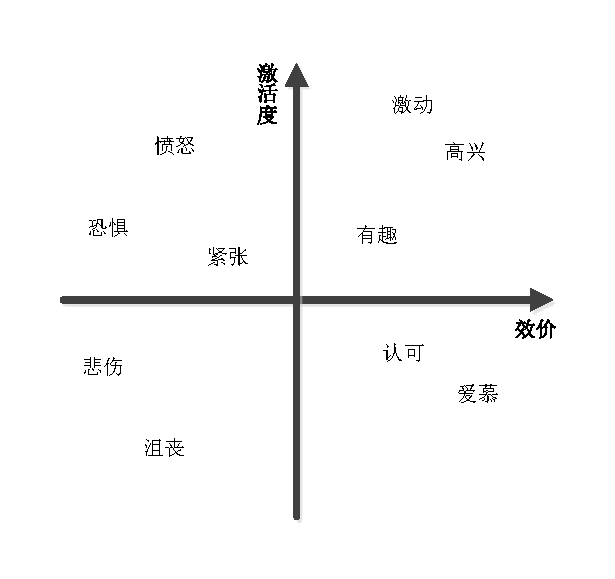
\includegraphics[height=10cm]{myfigures/emo_space_2dim}
    \caption{二维情感空间模型(激活度-效价)~\cite{Cowie2002Emotion}}
    \label{fig:emo_space_2dim}
\end{figure}

\begin{figure}[htb] % use float package if you want it here
    \centering
    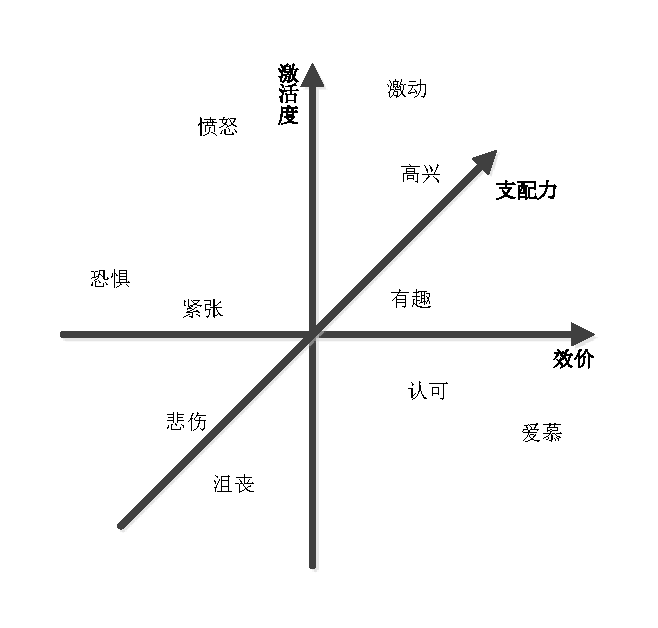
\includegraphics[height=10cm]{myfigures/emo_space_3dim}
    \caption{三维情感空间模型(激活度-效价-支配力)~\cite{Cowie2002Emotion}}
    \label{fig:emo_space_3dim}
\end{figure}

这种情感空间模型理论上可以描述任何情感,其中激活度代表情感的强烈程度,例如愤怒就是激活度非常高的情感。效价代表情感的积极性,例如悲伤就是一种积极性很低的情感,所以它的效价很低。支配力代表情感对别人的影响程度,例如高兴就是对别人影响比较大的一种情感,所以支配力比较大。情感空间模型将原先的标签分类问题转换为的对心理学属性值的回归问题,从而能够描述更为复杂的情感。但这种模型的的缺点是标记数据的成本太高,因为将主观情感量化为客观数值是一个繁重且难以保证质量的过程。

\section{情感语音数据库}
\label{sec:emo_speech_database}
在大多数的监督性机器学习问题中,训练数据一直是一个很大的问题,尤其是如何得到高质量的训练数据。对于语音情感识别而言,情感语音数据的获取和标注更是至关重要的问题。由于语音中情感信息的标注主要是要依靠人来完成的,但不同的人对情感的感知程度是不同的,所以同一句话有可能被不同的人标注为不同的情感。下面的两小节将主要介绍情感语音数据库的设计准则和一些常用的情感语音数据库。

\subsection{设计准则}
\label{ssec:design_criteria}
如何判断情感语音数据库能够模拟真实的应用场景,这需要相应设计准则来指导,下面将介绍几种主要的设计准则。

自然语音还是表演式语音?通常来说,最符合实际的语音数据应该是从日常生活的对话中收集~\cite{Campbell2000Databases},例如广播电台,电话客服系统等,这样的录音包含有最自然的情感表达。但不幸的是,由于一些法律和道德的原因,这样的数据被禁止用作研究目的。所以现在大多数情感语音数据库都采用了另一种替代方式,聘请一些专业的演员在录音室中去演绎预定的情感语音~\cite{Mazuka2015Emotions}。尽管有一些学者认为这样得到的语音情感表现过于夸张,和实际的自然语音不一致,但是这并不影响用这种数据库来探索声学表现和情感之间的相关性。

录制时如何唤醒情感?在录制情感语音数据库时,首先需要做的就是唤醒说话人的情感,通常有三种唤醒方式。第一种就是让说话人根据规定情感进行表演~\cite{Lee2005Toward},但这种方式得到情感表现过于夸张,和自然语音中的表现不一致。第二种就是将说话人置于某些特定的环境下来激起对特定的情感反应~\cite{Batliner2000Desperately},例如通过一些诱发式的交谈,或者一些交互式的游戏。第三种就是让标注者从生活中录制的自然语音去标注出有情感的句子~\cite{Johnstone2005Affective},这种语音最为真实,但是标注成本太高,需要大量的人力劳动。

不同情感的数据量是否平衡?由于在日常生活中,不同的情感触发的几率并不相同,所以会导致包含不同情感的语音数量也不同,例如中性语音是日常生活中出现最多的。这种分布不平衡的数据库会导致在训练分类器时出现偏置,使得分类器更趋向于预测为数据量多的那种情感。有一些数据库为了保持分布平衡会保证不同情感的句子数量基本一致~\cite{Burkhardt2005A}。但一些研究者~\cite{Hansen1997Getting, Morrison2007Ensemble}认为这种分布正体现了实际应用场景的情感出现概率,所以应该通过调整模型来包含这种信息。

情感语音是否应该保证说话人以及说话内容无关?由于不同的人表达情感的方式不相同,如果数据库中只包含个别人的语音就会导致模型不够强健,无法识别其他人的语音。应该保证尽可能多的说话人。还有就是语音中的语言学信息通常和情感都是强相关的,在录制数据库时是否应该排除掉语言学信息的影响,也是需要关注的问题。现在大多数研究者的观点是对于提前准备台词的表演型数据库,由于情感触发和文本是相关联的,所以并不适合用于语音情感识别。

\subsection{常用的情感语音数据库}
\label{ssec:available_database}
由于大多数的情感语音数据库都不是公开的,所以只有很少的基准数据库可以被研究者们共享。但由于情感语音数据的录制没有标准的规范,所以导致不同数据库的录制方式各不相同,下面的表格列举了一些常用的情感语音数据库。

\begin{table}[htb]
\centering
    \begin{minipage}[t]{1.0\linewidth} % 如果想在表格中使用脚注,minipage是个不错的办法
    \caption{常用的情感语音数据库}
    \label{tab:emo_database}
        % \begin{tabular}{p{6cm}<{\centering} p{6cm}<{\centering}}
        \begin{tabularx}{\linewidth}{X<{\centering} X<{\centering} X<{\centering} X<{\centering}}
            \toprule[1.5pt]
            数据库名 & 语言 & 大小 & 来源 \\
            \midrule[1pt]
            LDC~\cite{LibermanEmotional} & 英语 & 7人$\times$15种情感$\times$10个句子 & 专业演员 \\
            柏林情感语音数据库~\cite{Burkhardt2005A} & 德语 & 10人$\times$7种情感$\times$10个句子 & 专业演员 \\
            丹麦情感语音数据库~\cite{Engberg1997Design} & 丹麦语 & 4人$\times$5种情感 & 非专业演员 \\
            Natural~\cite{Morrison2007Ensemble} & 普通话 & 11人$\times$2种情感 & 呼叫中心 \\
            ESMBS~\cite{Nogueiras2012Speech} & 普通话 & 12人$\times$6种情感 & 非专业演员 \\
            INTERFACE~\cite{Hozjan2002Interface} & 英语,斯洛文尼亚语,西班牙语,法语 & 635个句子 & 专业演员 \\
            KISMET~\cite{Breazeal2002Recognition} & 美式英语 & 3人$\times$5种情感 & 非专业演员 \\
            BabyEars~\cite{Slaney2003Baby} & 英语 & 12人$\times$3种情感 & 父亲和母亲 \\
            SUSAS~\cite{Hansen1997Getting} & 英语 & 16000个句子 & 压力下的模仿 \\
            MPEG-4~\cite{Schuller2005Speaker} & 英语 & 2440个句子 & 美国电影 \\
            北航情感语音数据库~\cite{Fu2008Speaker} & 普通话 & 7人$\times$5种情感$\times$20个句子 & 非专业演员 \\
            FERMUS \uppercase\expandafter{\romannumeral3}~\cite{Schuller2002Towards} & 德话,英语 & 13人$\times$7种情感 & 诱发环境 \\
            KES~\cite{Kim2007Speech} & 韩语 & 5400个句子 & 非专业演员 \\
            CLDC~\cite{Zhou2006Speech} & 汉语 & 1200个句子 & 非专业演员 \\
            Pereira~\cite{Pereira2000Dimensions} & 英话 & 2人$\times$5种情感$\times$8个句子 & 非专业演员 \\
            IEMODB~\cite{Busso2008IEMOCAP} & 英话 & 10人$\times$9种情感 & 专业演员 \\
            \bottomrule[1.5pt]
        \end{tabularx}
    \end{minipage}
\end{table}

% \uppercase\expandafter{\romannumeral3}

这里主要介绍下IEMODB~\cite{Busso2008IEMOCAP}这个情感语音数据库,因为本文的研究工作主要是以这个数据库作为实验基础的。IEMODB主要被设计用于多模态情感表现研究,它包括肢体动作、音频和视频,一共有5个部分,每个部分包括10个主题,总共有接近12个小时的数据。每一个部分包含一个不同的对话场景,会有一个男演员和一个女演员分别表演规定好的剧本,以及在一个对话中诱发情感。至少三个标记员对同一句话标记情感类别,包括高兴、悲伤、中性、愤怒、惊讶、激动、沮丧、厌恶、恐惧这些情感标签。这个数据库被许多的研究工作采用,因此可以用来与其他研究工作的实验结果作对比。

\section{声学特征的抽取}
\label{sec:acoustic_feature_extract}
语音情感识别中一个重要的问题就是抽取与情感相关的声学特征,因为这些特征作为模型的输入会直接影响到最终的分类效果。下面将会对特征的选择和抽取方式做出介绍。

\subsection{人工选择情感相关的声学特征}
\label{ssec:artifical_select}
在大多数研究中,声学特征都是通过以往的一些经验选择或者设计出来的。用于语音情感识别的声学特征大致可以分为三类,分别为韵律学相关的特征、  谱相关的特征以及声音质量相关的特征,如图\ref{fig:acoustic_feature_type}所示。

\begin{figure}[htb] % use float package if you want it here
    \centering
    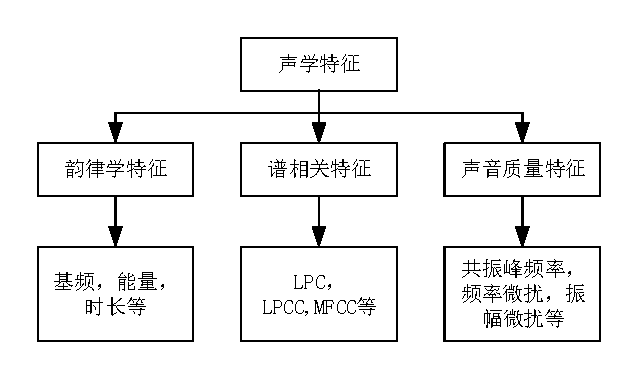
\includegraphics[height=9cm]{myfigures/acoustic_feature_type}
    \caption{不同类型的声学特征}
    \label{fig:acoustic_feature_type}
\end{figure}

韵律是指人说话时的节奏、轻重、快慢和音高等方面的的变化,它与语音中携带的语言学信息并没有太大的关联,但却决定着一句话给听众的感觉,因此又被称为“超音段特征”或“辅助语言学特征”。这种韵律学相关的特征被广泛的应用在语音情感识别领域,主要包括基频、时长、能量等。根据Williams和Stevens的研究~\cite{Williams1981Vocal},语音情感的激活度会显著的影响频谱上的能量分布、基频的大小以及停顿的时长,其他一些研究~\cite{Johnstone2000Vocal, Cowie2003Describing}也证明了这一结论。此外,有研究证明这些特征也和基本情感类别有着很强的关联,例如Murray和Arnott的研究~\cite{Murray1993Toward}证明快的说话速率与愤怒是相关联的,但也有些研究~\cite{Ackroyd1997Digital, Cahn1990The}表明部分情感的韵律学比较相似,例如愤怒、恐惧、高兴和惊讶都有相似的基频。

谱相关的特征被认为与声道对语音信号的调制相关联,这类特征之前一直被语音识别广泛的应用,但现在一些研究证明这类特征在情感识别中也发挥很大的作用,例如线性预测系数(Linear Prediction Coefficients, LPC)~\cite{Ackroyd1997Digital},线性预测倒谱系数(Linear Prediction Cepstral Coefficients, LPCC)~\cite{Atal1974Effectiveness}以及梅尔频率倒谱系数(Mel-frequency Cepstral Coefficients, MFCC)~\cite{Rabiner1999Fundamentals, Proakis1993Discrete}。Nwe等人~\cite{Nogueiras2012Speech}发现语音信号不同频段的能量分布和情感类别有着相关性,例如高兴的语音通常在高频段有着较高的能量,而悲伤的语音在高频段的能量却相对较低。

声音质量特征是人对声音的一种主观评价,主要用于衡量声音的流利和清晰程度。当人在情绪比较激动的时候,通常会出现哽咽、颤音、喘息之类的反应,这会导致声音质量发生变化。因此,研究者~\cite{Gobl2003The}认为声音质量特征也可以反映情感的变化。声音质量特征包括共振峰频率及其带宽、频率微扰、振幅微扰、声门参数等。Lugger等人~\cite{Lugger2007The, Lugger2008Psychological, Lugger2015Combining}通过使用共振峰频率和带宽作为特征取得了很不错的效果。Li等人~\cite{Li2007Stress}也采用梅尔频率倒谱系数加频率微扰和振幅微扰,取得超过只使用梅尔频率倒谱系数的效果。

\subsection{特征选择算法筛选情感相关的声学特征}
\label{ssec:algorithm_select}
声学特征有许多种,选择与情感相关的特征除了依靠人工挑选以外,还可以通过一些特征选择算法来自动选出相关的特征。假设我们有一个很大的特征集合,特征选择算法所要做的就是规定一种指标,例如熵增益~\cite{Dhillon2003A}或者识别准确率~\cite{Dietterich1998Approximate},然后通过特征的各种组合来选取出那些指标最好的特征子集。这样既可以减少输入特征的数量,降低计算量,又可以去除无效特征的干扰,大致流程如图\ref{fig:feature_select_flow}所示。

\begin{figure}[htb] % use float package if you want it here
    \centering
    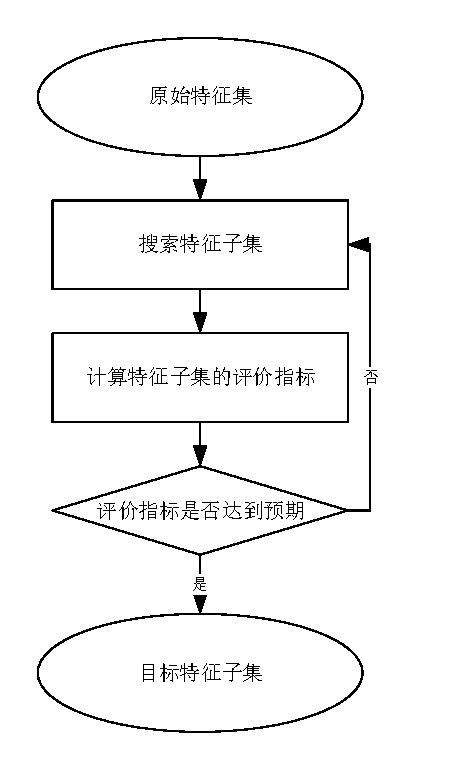
\includegraphics[height=14cm]{myfigures/feature_select_flow}
    \caption{特征选择流程图}
    \label{fig:feature_select_flow}
\end{figure}

特征选择算法有许多,例如序列浮动前向选择算法(Sequential Floating Forward Selection, SFFS)~\cite{Ververidis2008Fast}通过迭代的方法选择出接近最优的特征子集;还有遗传算法(Genetic Algorithm, GA)~\cite{Yang1998Feature}是一种模拟生物进化的算法,它通过不断地繁殖和变异来筛选出最优的特征子集。除了特征选择算法以外,还有一些特征空间转换的算法也可以降低输入特征的维度,例如主成分分析(Principal Component Analysis, PCA)~\cite{Ben2003Detecting}和线性判别分析(Linear Discriminant Analysis, LDA)~\cite{Blum1997Selection},它们可以通过矩阵运算将高维特征向量转换到低维特征向量,从而减少计算量。


\subsection{深度神经网络抽取情感相关的声学特征}
\label{ssec:dnn_extract}
在近几年,深度学习方法和工具被引入到语音信号处理领域~\cite{Han2014Speech, Lee2015High, Huang2014Speech, Le2013Emotion, Rana2016Emotion, Chernykh2017Emotion},研究者发现采用深度神经网络从原始语音信号来提取特征,可以取得比人工定义的声学特征更好的结果,同时这也衍生出了端到端语音情感识别系统。现在有很多的神经网络结构都被用于特征抽取,例如最早的工作是Jaitly等人~\cite{Jaitly2011Learning}通过受限玻尔兹曼机(Restricted Boltzmann Machine, RBM)从原始语音信号上得到一种有利于语音识别的中间表示。Bhargava等人~\cite{Bhargava2015Architectures}则是通过堆叠的全连接神经网络从原始语音信号得到瓶颈特征,并且取得了和使用梅尔频率倒谱系数(Mel-frequency Cepstral Coefficients, MFCC)相近的效果。George等人~\cite{Trigeorgis2016Adieu}提出一种使用卷积神经网络(Convolution Neural Network, CNN)从原始语音信号提取特征,然后通过长短时记忆循环神经网络(Long-Short Term Memory Recurrent Neural Network, LSTM-RNN)捕获输入序列的时序信息并最终输出不同情感的后验概率,并且他们发现长短时记忆循环神经网络(Long-Short Term Memory Recurrent Neural Network, LSTM-RNN)不同节点的输出和一些声学特征有很强的相关性。Satt等人~\cite{Satt2017Efficient}也采用了相似的神经网络结构,但不同的是他们从语谱图上抽取特征而非原始语音信号。他们认为在语谱图上可以更方便的进行去噪的操作,并且他们在公开情感语音数据集IEMOCAP上取得了超过之前最好结果(state-of-the-art)的准确率。

\section{情感分类模型的构建}
\label{sec:emotion_cls}

在抽取声学特征之后,需要构建分类模型来判别特征向量所属的情感类别。事实上,目前情感语音识别的大多数研究都是关注在这一步骤上,下面我们将介绍情感分类模型的相关的技术,主要包括传统的分类模型和深度学习的分类模型。

\subsection{基于传统机器学习的情感分类模型}
\label{ssec:traditional_cls}

许多传统机器学习中的分类算法已经被运用在语音情感识别任务上,例如隐马尔可夫模型(Hidden Markov Model, HMM),高斯混合模型(Gaussian Mixture Models, GMM),支持向量机(Support Vector Machine, SVM)等。目前并没有公认的最适合语音情感识别的分类器,每一种分类器都有各自的优缺点,下面我们将分别介绍几种常用的分类器模型。

HMM被广泛地应用在语音识别领域,例如孤立词的识别和端点检测。这是因为它和语音信号的产生机制十分相似~\cite{Rabiner2007An}。HMM是一个包含一阶马尔科夫链的双随机过程,分别包含隐藏的转移状态和可观测的输出,其中隐藏状态是用来建模语音信号的时序信息。在数学上,为了通过HMM给一个可观测序列$\mathbf{x}_1,...,\mathbf{x}_T$建模,我们假设一个马尔科夫链可以用于生成观测序列,让$K$代表状态的数量,$\pi_i, i=1,...,K$代表不同状态的初始概率,$a_{ij}, i=1,...K, j=1,...,K$代表从状态$i$到状态$j$的转移概率。通常HMM的参数都是通过最大似然的方法来估计。假设实际的状态序列是$s_1,...,s_T$,观测序列的似然度可以通过下面的公式给出:
\begin{equation}
\label{equ:output_pro}
    \begin{aligned}
        p(\mathbf{x}_1,s_1,...,\mathbf{x}_T,s_T) &= \pi_{s_1}b_{s_1}(\mathbf{x}_1)a_{s_1,s_2}b_{s_2}(\mathbf{x}_2)...a_{s_{T-1},s_T}b_{s_T}(\mathbf{x}_T) \\
        &= \pi_{s_1}b_{s_1}(\mathbf{x}_1)\prod\limits_{t=2}^Ta_{s_{t-1},s_t}b_{s_t}(\mathbf{x}_t)
    \end{aligned}
\end{equation}
其中,$b_i(\mathbf{x}_t) \equiv P(\mathbf{x}_t|s_t = i)$是第$i$个状态的输出概率。它既可以是离散的概率分布,也可以是连续的概率密度。因为真实的状态序列并不知道,所以在给定输出序列时,我们必须对所有可能的状态序列的似然度求和,如下面的公式:
\begin{equation}
\label{equ:output_pro_sum}
        p(\mathbf{x}_1,...,\mathbf{x}_T) = \sum\limits_{s_1,...,s_T}\pi_{s_1}b_{s_1}(\mathbf{x}_1)\prod\limits_{t=2}^Ta_{s_{t-1},s_t}b_{s_t}(\mathbf{x}_t)
\end{equation}
幸运的是,一种计算似然度的高效算法已经提出,可以将时间复杂度降低至$O(KT)$。在训练阶段,HMM的参数通过最大化公式\ref{equ:output_pro_sum}的似然度来获得,这通常可以使用期望最大化(Expectation Maximization, EM)算法~\cite{Dempster1977Maximum}来实现。在语音识别中,HMM的结构通常是从左到右的,因为这种结构符合语音信号的时序特性。但在语音情感识别中,除了使用从左到右结构以外,全连接的结构也会被使用,因为情感信息可能只集中在某一个小的时间段内,而不是所有的时间段都是均匀的。HMM已经被许多语音情感识别的研究所采用, 在Nwe的工作~\cite{Nogueiras2012Speech}中,一个基于HMM的语音情感识别系统用于区分6种基本情感,模型为不同的情感和不同的说话人分别构建了一个四状态的全连接HMM。在Lee的工作~\cite{Lee2004Emotion}中,两个不同的HMM模型被提出,一种是普通的HMM加GMM的模型,另一种则是和语音识别一样先构建对音素的HMM模型,然后构建音素序列到情感类别的映射模型,作者表示采用对音素建模的方式比普通的方式可以取得更好的效果。

GMM是一种采用多个高斯分布变量的概率模型,它可以被考虑为一种只包含一个状态的HMM~\cite{Vlassis2002A, Reynolds1995Robust}。GMM的训练和测试过程相比于一般的连续HMM更为简单,这也使得它被广泛的使用在语音情感识别中,但是GMM无法建模语音信号的时序信息。在GMM模型构建中最困难的就是决定需要多少个高斯分量,最简单的方法就是人工尝试设置不同的数量,然后看模型的效果。此外,期望最大化算法可以被用来自动调整高斯分量的数量和模型的参数。GMM相关的工作也有许多,在Breazeal的工作~\cite{Breazeal2002Recognition}中,一个GMM分类器被用在KISMET情感语音数据库上,获得了77.87\%的平均准确率,后面又采用分层决策的策略取得了81.94\%的平均准确率。GMM也被用在其他的情感语音数据库中,例如BabyEars情感语音数据库~\cite{Slaney2003Baby},模型尝试了1-100的高斯分量数量,最终在数量为10的时候取得了最好的结果,达到平均准确率为75\%。在FERMUS \uppercase\expandafter{\romannumeral3}数据库上也获得相似的结果,16个分量的GMM被用来为每种情感建模,平均准确率达到了74.83\%。

SVM是一种非常流行的分类算法~\cite{Burges2008A},它在许多的模式识别任务中均取得了很不错的效果。SVM模型主要是利用核函数将在低维特征空间线性不可分的向量映射到高维空间,使得数据可以被线性分类器划分。相比于HMM和GMM,SVM可以得到全局最优的分类边界~\cite{Burges1998A},但是对于不可分的数据,它又不得不采用一些启发式的方法。事实上,并没有系统性的方法可以用来选择核函数,因此,转换后的数据可分性是无法保证的。在大多数模式识别任务,包括语音情感识别,并不建议找到训练数据的最佳分类面,因为这可能会导致过拟合。有许多语音情感识别的研究都在使用SVM~\cite{Lee2004Emotion, Schuller2004Speech, Kwon2003Emotion, Pierre2003The},它们都取得了相似的结果。其中一个工作将SVM通过三种不同的策略从二分类器转换为多分类器。第一种策略是将多分类任务转换为多个二分类任务,每个二分类任务将一个情感看作一类,其他所有情感看作一类,所有二分类器的结果中输出最大的情感类别代表最终的识别结果。第二种策略是将所有二分类器的输出传递给一个三层感知机,让它完成最后的决策。第三种方法是采用分层决策的策略,在不同的阶段决策不同的情感。这三种模型在FERMUS \uppercase\expandafter{\romannumeral3}数据库上做测试,分别得到了76.12\%,75.45\%和81.29\%的分类准确率。

除了采用单一的分类模型以外,多分类器混合模型也被用于语音情感识别。有三种不同的方法来组合不同的分类器~\cite{Kuncheva2004Combining, Lugger2015Combining}。第一种是分层判决的方法,每个分类器都被放置在一棵决策树的各个节点,输入从根节点出发,不断向下探索,最终到达叶子节点时会被划分到唯一的情感类别。在Lugger的工作~\cite{Lugger2008Psychological}中,分层的模型在柏林情感语音数据库中测试,其中采用了考虑心理学情感属性的二阶段和三阶段分层分类系统。二阶段的方法可以达到83.5\%的分类准确率,三阶段的方法可以达到88.8\%的分类准确率。第二种是顺序串行的判决方法,就是依次采用不同的分类器对数据进行分类,当前的分类器会影响下一个分类器的结果。第三种是多分类器并行的判决方法,就是同时训练多个分类器,然后将所有分类器的结果进行决策融合得到最终的分类结果。

\subsection{基于深度学习的情感分类模型}
\label{ssec:dnn_cls}

近几年来,深度学习的模型开始变的越来越流行,这种方法也在语音情感识别中也取得了很不错的效果。相比于传统的机器学习模型,深度学习模型可以对更复杂的非线性映射关系进行建模。已经有许多的深度神经网络结构被提出,例如自编码神经网络(Auto-Encode Neural Network),卷积神经网络(Convolution Neural Network, CNN),循环神经网络(Memory Recurrent Neural Network, RNN),受限玻尔兹曼机(Restricted Boltzmann Machine, RBM)等。其中一部分工作仍然是采用传统的声学特征来进行建模,但近几年也开始出现直接基于原始信号的端到端的语音情感识别。

基于传统声学特征的深度学习分类模型已经有很多工作,Han等人~\cite{Han2014Speech}采用普通的深度神经网络(Deep Neural Network, DNN)得到不同的语音子段在不同情感上的概率分布,然后通过统计学方法的方法将所有子段的概率分布融合得到整个句子的特征表示,最后采用一种单层的神经网络结构,叫做极限学习器(Extreme Learning Machine, ELM)来得到最终的情感类别。在IEMOCAP数据库~\cite{Busso2008IEMOCAP}上,这种方法取得了48.2\%的不加权准确率(Unweighted Accuracy, UA)和54.3\%的加权准确率(Weighted Accuracy, WA)。Kim等人~\cite{Kim2013Deep}提出采用深度信念网络(Deep Belief Network, DBN)代替传统的特征选择算法,来获得更为有效的特征表示。 DBN是由多层RBM堆叠而成,可以采用无监督的方式训练,在IEMOCAP数据库~\cite{Busso2008IEMOCAP}上取得了66.12\%的不加权准确率。Deng等人~\cite{Deng2013Sparse}采用一种自编码神经网路来进行特征的转换学习,他们先通过大量未标记的情感语音训练自编码神经网络,从而可以找到更为有效的特征表示,然后再用标记数据对自编码神经网络进行微调,在5个不同的情感语音数据库上进行交叉测试均取得了不错的效果。

基于原始信号的端到端的分类模型也开始有一些工作被提出。George等人~\cite{Trigeorgis2016Adieu}提出使用CNN从原始语音信号提取特征,然后通过LSTM-RNN捕获输入序列的时序信息并最终输出不同情感的后验概率。作者认为通过CNN和RNN可以将时序信息编码到特征表示中,并且他们发现LSTM-RNN不同节点的输出和一些传统的声学特征有很强的相关性。实验结果表明这种端到端的方式可以取得比传统声学特征更好的效果。Satt等人~\cite{Satt2017Efficient}也采用了相似的神经网络结构,但不同的是他们从语谱图上抽取特征而非原始语音信号。他们认为在语谱图上可以更方便的进行去噪的操作,并且他们在公开情感语音数据集IEMOCAP~\cite{Busso2008IEMOCAP}上取得了超过之前最好结果(The State of Art)的准确率。

\section{本章小结}
\label{sec:basic_konwledge_summary}

本章简单介绍了语音情感识别相关的研究工作,包括情感的定义、情感语音数据库、情感相关的声学特征和一些常用的情感分类模型。这些工作包含了当前语音情感识别领域的主要关注点,为后面介绍自己的研究工作提供了铺垫。

% \chapter{中华人民共和国}
% \label{cha:china}

% \section{其它例子}
% \label{sec:other}

% 在第~\ref{cha:intro} 章中我们学习了贝叶斯公式~(\ref{equ:chap1:bayes}),这里我们复
% 习一下:
% \begin{equation}
% \label{equ:chap2:bayes}
% p(y|\mathbf{x}) = \frac{p(\mathbf{x},y)}{p(\mathbf{x})}=
% \frac{p(\mathbf{x}|y)p(y)}{p(\mathbf{x})}
% \end{equation}

% \subsection{绘图}
% \label{sec:draw}

% 本模板不再预先装载任何绘图包(如 \pkg{pstricks,pgf} 等),完全由用户来决定。
% 个人觉得 \pkg{pgf} 不错,不依赖于 Postscript。此外还有很多针对 \LaTeX{} 的
%  GUI 作图工具,如 XFig(jFig), WinFig, Tpx, Ipe, Dia, Inkscape, LaTeXPiX,
% jPicEdt, jaxdraw 等等。

% \subsection{插图}
% \label{sec:graphs}

% 强烈推荐《\LaTeXe\ 插图指南》!关于子图形的使用细节请参看 \pkg{subcaption} 宏包的说明文档。

% \subsubsection{一个图形}
% \label{sec:onefig}
% 一般图形都是处在浮动环境中。之所以称为浮动是指最终排版效果图形的位置不一定与源文
% 件中的位置对应\footnote{This is not a bug, but a feature of \LaTeX!},这也是刚使
% 用 \LaTeX{} 同学可能遇到的问题。如果要强制固定浮动图形的位置,请使用 \pkg{float} 宏包,
% 它提供了 \texttt{[H]} 参数,比如图~\ref{fig:xfig1}。
% \begin{figure}[H] % use float package if you want it here
%   \centering
%   
\includegraphics{thu-whole-logo}
%   \caption{利用 Xfig 制图}
%   \label{fig:xfig1}
% \end{figure}

% 大学之道,在明明德,在亲民,在止于至善。知止而后有定;定而后能静;静而后能安;安
% 而后能虑;虑而后能得。物有本末,事有终始。知所先后,则近道矣。古之欲明明德于天
% 下者,先治其国;欲治其国者,先齐其家;欲齐其家者,先修其身;欲修其身者,先正其心;
% 欲正其心者,先诚其意;欲诚其意者,先致其知;致知在格物。物格而后知至;知至而后
% 意诚;意诚而后心正;心正而后身 修;身修而后家齐;家齐而后国治;国治而后天下
% 平。自天子以至于庶人,壹是皆以修身为本。其本乱而未治者 否矣。其所厚者薄,而其所
% 薄者厚,未之有也!

% \hfill —— 《大学》


% \subsubsection{多个图形}
% \label{sec:multifig}

% 如果多个图形相互独立,并不共用一个图形计数器,那么
% 用 \texttt{minipage} 或者\texttt{parbox} 就可以。否则,请参看
% 图~\ref{fig:big1-subcaptionbox},它包含两个小图,分别是图~\ref{fig:subfig1}和
% 图~\ref{fig:subfig2}。推荐使用 \cs{subcaptionbox},因为可以像
% 图~\ref{fig:big1-subcaptionbox} 那样对齐子图的标题,也可以使用 \pkg{subcaption}
% 宏包的 \cs{subcaption}(放在 minipage中,用法同\cs{caption})或
% 是 \pkg{subfigure} 、\pkg{subtable}环境,像图~\ref{fig:big1-subfigure},不要再
% 用 \cs{subfloat}、\cs{subfigure} 和 \cs{subtable}。

% \begin{figure}[h]
%   \centering%
%   \subcaptionbox{第一个小图形\label{fig:subfig1}}[3cm] %标题的长度,超过则会换行,如下一个小图。
%     {
\includegraphics[height=3cm]{thu-fig-logo}}%
%   \hspace{4em}%
%   \subcaptionbox{第二个小图形,注意这个图略矮些。如果标题很长的话,它会自动换行\label{fig:subfig2}}
%       {
\includegraphics[height=2cm]{thu-text-logo}}
%   \caption{包含子图形的大图形(subcaptionbox示例)}
%   \label{fig:big1-subcaptionbox}
% \end{figure}
% \begin{figure}[h]
%   \centering%
%   \begin{subfigure}{3cm}
%     
\includegraphics[height=3cm]{thu-fig-logo}
%     \caption{第一个小图形}
%   \end{subfigure}%
%   \hspace{4em}%
%   \begin{subfigure}{0.5\textwidth}
%     
\includegraphics[height=2cm]{thu-text-logo}
%     \caption{第二个小图形,注意这个图略矮些。subfigure中同一行的子图在顶端对齐。}
%   \end{subfigure}
%   \caption{包含子图形的大图形(subfigure示例)}
%   \label{fig:big1-subfigure}
% \end{figure}

% 古之学者必有师。师者,所以传道受业解惑也。人非生而知之者,孰能无惑?惑而不从师,
% 其为惑也,终不解矣。生乎吾前,其闻道也固先乎吾,吾从而师之;生乎吾後,其闻道也亦
% 先乎吾,吾从而师之。吾师道也,夫庸知其年之先後生於吾乎!是故无贵无贱无长无少,道
% 之所存,师之所存也。

% 嗟乎!师道之不传也久矣,欲人之无惑也难矣。古之圣人,其出人也远矣,犹且从师而问焉;
% 今之众人,其下圣人也亦远矣,而耻学於师。是故圣益圣,愚益愚。圣人之所以为圣,愚
% 人之所以为愚,其皆出於此乎?爱其子,择师而教之,於其身也,则耻师焉,惑焉。彼童子
% 之师,授之书而习其句读者,非吾所谓传其道、解其惑者也。句读之不知,惑之不解,或师
% 焉,或不焉,小学而大遗,吾未见其明也。巫医、乐师、百工之人不耻相师,  士大夫之族
% 曰“师”曰“弟子”之云者,则群聚而笑之。问之,则曰:彼与彼年相若也,道相似也,位
% 卑则足羞,官盛则近谀。呜呼!师道之不复,可知矣。巫医、乐师、百工之人。吾子不齿,
% 今其智乃反不能及,其可怪也欤!圣人无常师。孔子师郯子、苌子、师襄、老聃。郯子之徒,
% 其贤不及孔子。孔子曰:“三人行,必有我师。”是故弟子不必不如师,师不必贤於弟子。
% 闻道有先後,术业有专攻,如是而已。

% 如果要把编号的两个图形并排,那么小页就非常有用了:
% \begin{figure}
% \begin{minipage}{0.48\textwidth}
%   \centering
%   
\includegraphics[height=2cm]{thu-whole-logo}
%   \caption{并排第一个图}
%   \label{fig:parallel1}
% \end{minipage}\hfill
% \begin{minipage}{0.48\textwidth}
%   \centering
%   
\includegraphics[height=2cm]{thu-whole-logo}
%   \caption{并排第二个图}
%   \label{fig:parallel2}
% \end{minipage}
% \end{figure}

% 李氏子蟠,年十七,好古文、六艺,经传皆通习之,不拘於时,学於余。余嘉其能行古
% 道,作师说以贻之。

% \hfill —— 韩愈(唐)

    \chapter{基于情感对的语音情感识别框架}
\label{cha:emo_pair_base_framework}

\section{本章引论}
\label{sec:emo_pair_base_framework_intro}
特征选择作为传统语音情感识别中一个重要的部分,已经吸引了许多研究者的关注。因为情感是人类的主观感受,想要通过声音中的线索来反映当前说话人的情感状态是一个非常具有挑战性的任务。目前大多数的研究都旨在为所有的情感类别找到一个统一的特征集合,因为在一个共同的特征集合上构建分类器也是通常处理多分类问题的方法。但是一些研究结果~\cite{Lee2009Emotion}已经证明与不同的情感相关的声学特征也是不同的,也就是说为所有的情感选择相同的特征集合并不是一个很好的方法;相反,为特定的情感选择特定的特征集合可以取得更好的效果。

基于上述原因,我们认为给不同的情感组合选择相关程度最高的的特征空间,保证这些情感在这样的特征空间上具有更高的可分性,是一个比较适合的实现方式。为此,我们提出了一种基于情感对的语音情感识别框架。本章的剩余部分是这样安排的:首先我们将介绍基于情感对的识别框架如何构建;接下来我们详细介绍情感对的定义,基于情感对的特征选择算法,和基于情感对的二分类模型;然后,我们将介绍决策融合的方法,包括基于投票的决策融合和基于情感空间的贝叶斯决策融合;最后,我们将本文所提方法与采用全局特征集合的方法、以及基于层次分类的方法进行实验对比。

\section{基于情感对的识别框架}
\label{sec:emo_pair_base_framework}
我们将任意两种不同的情感组成情感对,然后为每一个情感对选择最相关的声学特征子集。这种特征选择方式将在很大程度上缩减需要处理的问题域,因为现在我们将之前需要为多种情感选择特征的问题转换为为两种情感选择特征的问题,剔除了许多无关的干扰特征。当为每一个情感对选择出对应的特征子集之后,我们将在每个特征子集上构建二分类器,这样就将原本的多分类问题转换为多个二分类问题。此时,又存在一个问题,就是最后我们期望的结果是一句话只得到一个识别结果,但现在每个二分类器都会得到一个结果,所以我们还需要再加入一个决策融合的步骤。最简单的决策融合方法就是采用投票策略,将所有二分类器的结果中出现次数最多的那个情感作  为最终的识别结果。但投票的策略存在两个缺点,一是会出现票数相同的问题,二是只有和目标情感相关的那些二分类结果才有贡献,其他的二分类结果只会产生干扰。为了避免这两个缺点,我们引入情感空间模型中不同情感之间的距离信息,通过贝叶斯分类器来完成决策融合的步骤,整个系统的流程图如图\ref{fig:emo_pair_flow}所示。

\begin{figure}[htb] % use float package if you want it here
    \centering
    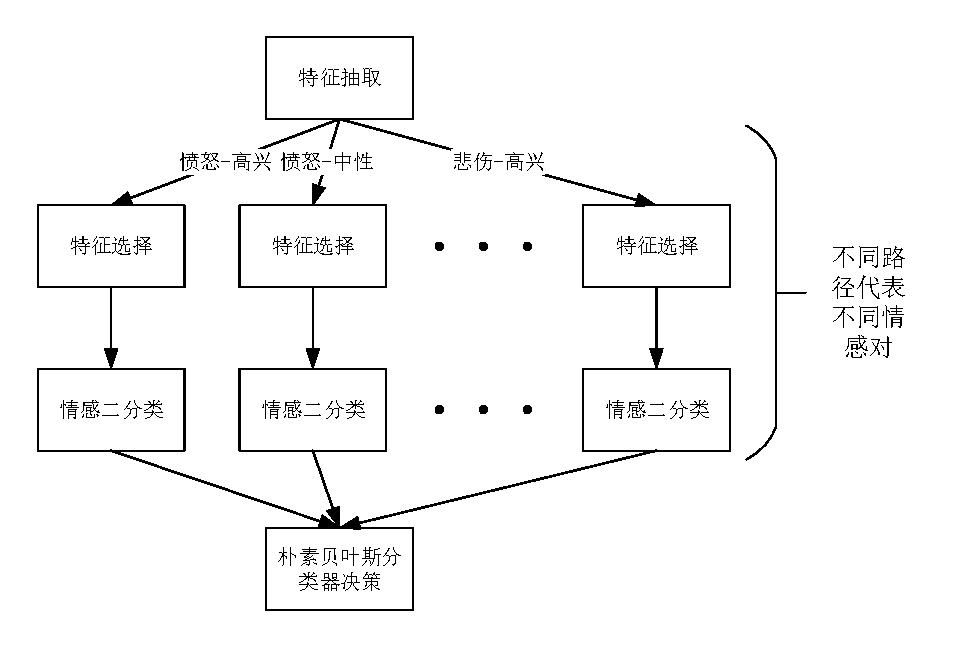
\includegraphics[height=10cm]{myfigures/emo_pair_flow}
    \caption{基于情感对的识别框架}
    \label{fig:emo_pair_flow}
\end{figure}

基于层次的语音情感识别框架~\cite{Lee2009Emotion}和我们的设计有着相似的思想,都是期望为不同的情感类别采用不同的特征集合,但是我们的方法效果更好,而且当情感类别发生变化时更容易扩展。此外,由于多个二分类任务之间没有依赖关系,所以更易于并行加速。

\section{情感对二分类}
\label{sec:emo_pair}

\subsection{情感对的定义}
\label{ssec:emo_pair_def}
任意两个不相同的情感组合在一起就被称为情感对。这种思想是源于集成学习(Ensemble Learning)~\cite{Liu1999Ensemble}的一些观点。集成学习大致可以分为两种方式,一种被称为引导聚合(Bootstrap Aggregating, Bagging),这种方法利用重采样的方法从整体数据集中进行有放回的抽样得到N个数据集,在每个数据集上学习出一个模型,最后的预测结果利用N个模型的结果共同决策得到,例如随机森林(Random Forest)~\cite{Liaw2002Classification}就属于这种方法。总的来说,引导聚合先训练多个简单的弱分类器,然后通过这些弱分类器组合成一个强分类器。另一种被称为提升方法(Boosting),这种方法是一种可以减小监督学习中偏差的机器学习算法。主要原理也是学习一系列弱分类器,并将其组合成一个强分类器,其中最具代表性的方法是AdaBoost (Adaptive Boosting)算法~\cite{Ratsch2001Soft},这种算法在刚开始训练时对每一个训练样例赋相同的权重,然后对训练集进行多轮迭代训练,每轮训练结束后都对预测错误的那些样例赋以较大的权重,也就是让学习算法以后更注意学错的样本,从而可以得到多个预测模型,最终再以正比于准确率的权重将所有模型的结果组合到一起得到最后的结果。

我们提出的情感对有些类似于引导聚合的思想,首先为不同的情感对分别选择特征和训练分类器,最后再将所有分类器的结果融合到一起。由于每个情感对只需要为两种情感选择相关的特征,相比于为所有的情感选取相关的特征,这大大减少了干扰特征的引入。

同情感对相似思想的还有基于层次的语音情感识别方法~\cite{Lee2009Emotion},这种方法首先会根据观察设计一棵二叉决策树,在树中的不同节点分别区分不同的情感类别或情感类别组,并且每一个节点的分类器都是单独选择特征集的。情感类别组是指将多种情感分别归属到两个不同的组中,然后将这两个组看做两个类。识别过程是从根节点开始进行分类,自顶向下沿着路径上的节点依次进行分类,最后到达叶子节点后将会得到一种唯一的情感,整个分类流程如图\ref{fig:hierarchical_flow}所示。但这个方法有两个缺点,第一是整个决策树的结构需要人工来设计,当情感类别或应用场景发生变化时,整个决策树就得重新设计,并不具备通用性。第二是由于整个分类过程是自顶向下的,所以会存在错误累积的问题,就是说如果上一层的分类结果是错误的,这些错分的样本就会沿着路径一直走下去,从而影响下层节点的分类效果。

我们基于情感对的方法则可以解决这两个问题,首先情感对的方法不需要任何的人工介入,因为情感对只是将任意两种情感组合到一起,即使需要加入新的情感类别,仅仅只是需要生成新的情感对,之前已经训练好的二分类模型仍然可以使用,这将大大减少训练时间。其次,情感对的方法不存在错误累积问题,因为不同的情感对之间的输入都是独立的,不会相互产生影响。此外,由于不同情感对之间没有依赖关系,所以训练可以并行完成,这将进一步提升训练速度。

\begin{figure}[htb] % use float package if you want it here
    \centering
    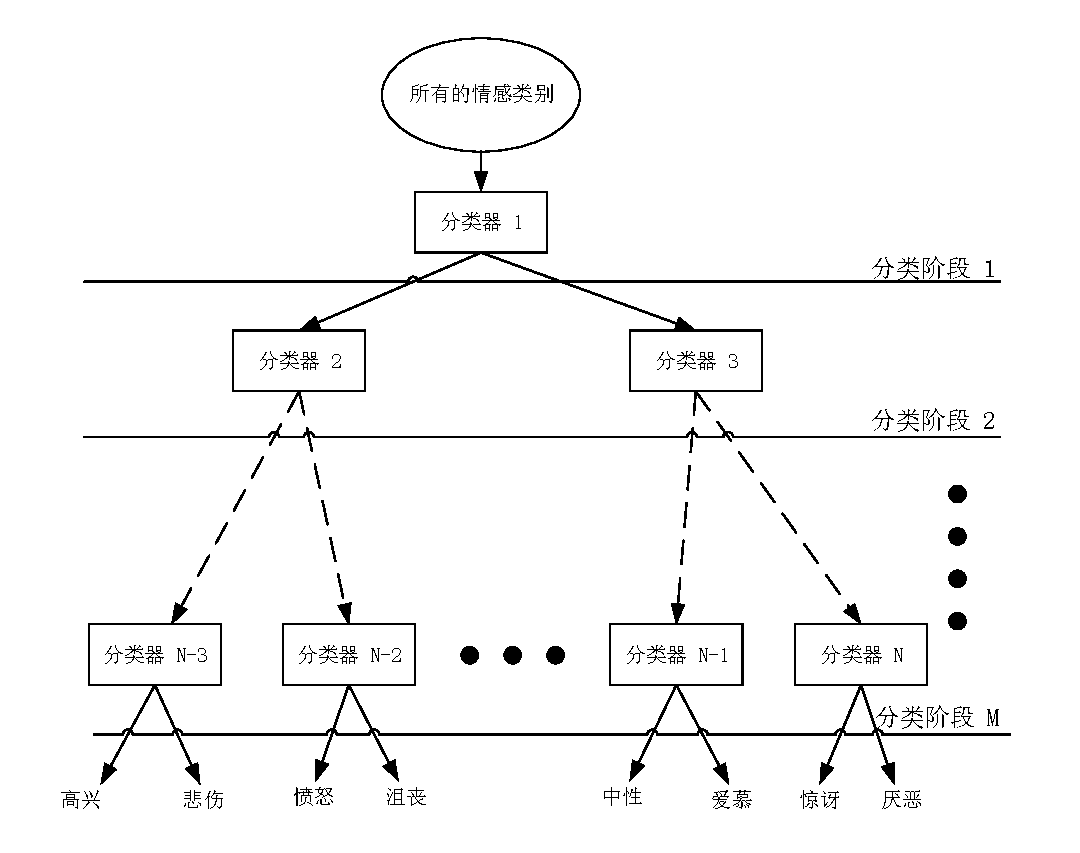
\includegraphics[height=10cm]{myfigures/hierarchical_flow}
    \caption{基于分层决策树的识别框架}
    \label{fig:hierarchical_flow}
\end{figure}

下面两小节我们将专门针对基于情感对的声学特征选择算法和二分类模型做出详细的阐述,这两个问题是整个识别框架中最关键的问题。

\subsection{基于情感对的声学特征选择}
\label{ssec:emo_pair_feature_select}
特征选择算法有许多,这些算法的目的主要可以分为三个方面:第一是提升模型的预测准确率;第二是筛除无用的冗余特征,减少计算时间;第三是针对当前的问题域,对于数据提供一个更好的理解。下面将会对特征选择指标,特征选择策略以及基于情感对的特征选择实现这三个方面分别作介绍。

\subsubsection{特征评价指标}
\label{sssec:feature_select_metrics}
对于特征选择算法来说最重要的是要选取一种指标来衡量选出的特征的好坏。假设我们有一个含有$m$个样例的数据集$\{\mathbf{x}_k, y_k\}(k=1,...,m)$,每个样例包含$n$个输入特征$x_{k,i}(i=1,...,n)$和一个输出值$y_k$,第$i$个特征的评判指标通过函数$S(i)=f(\{x_{k,i}, y_k\}(k=1,...,m))$来定义。一般来说,我们定义$S(i)$越大的特征和任务目标越相关。为了方便下面的解释,我们再引入一些其他的定义:如果输入向量$\mathbf{x}$被看做来自一个潜在的多变量概率分布$\mathbf{X}$,我们定义$X_i$代表$\mathbf{x}$中第$i$个特征的随机变量。同样,$Y$代表输出值$y$的随机变量。进一步,我们定义$m$维的向量$\mathbf{x}_i$代表数据集中第$i$个特征的所有值,$m$维的向量$\mathbf{y}$代表数据集中所有样本的输出值。

第一种特征评价指标叫做相关系数~\cite{Weston2003Use},我们假设输出$y$是一个连续值,则泊松相关系数被定义为:
\begin{equation}
\label{equ:pearson_cc}
    \Re(i) = \frac{cov(X_i, Y)}{\sqrt{var(X_i)var(Y)}}
\end{equation}
$cov$代表协方差,$var$代表方差。通过统计方法对$\Re(i)$的估计$R(i)$可以表示为:
\begin{equation}
\label{equ:pearson_cc_real}
    R(i) = \frac{\sum_{k=1}^{m}(x_{k,i} - \overline{x_i})(y_k - \overline{y})}{\sqrt{\sum_{k=1}^{m}(x_{k,i} - \overline{x_i})^2}\sum_{k=1}^{m}(y_k - \overline{y})^2}
\end{equation}
符号上面的横线代表对所有的下标$k$求平均值,这个系数也可以看作向量$\mathbf{x}_i$和向量$\mathbf{y}$的余弦值。在线性回归中,评价指标通常是$R(i)$的平方,这样将可以去除负值,仅仅表示向量$\mathbf{x}_i$和向量$\mathbf{y}$的线性相关性。此外,相关系数$R(i)$仅仅可以表示特征和目标之间的线性依赖关系,如果希望可以获取非线性关系,最简单的方法就是对输入进行非线性的处理。例如取平方、开方、取对数等等。

第二种方法是采用单变量分类器~\cite{Forman2003An},这种方法是将一个特征输入一个分类器中,然后将分类器的预测能力作为衡量指标。通常用来衡量分类器的预测能力的指标是错误率,例如对于二分类问题,错误的识别为正例的比率(Fasle Positive Rate, FPR)和错误识别为负例的比率(False Negative Rate, FNR)都可以被被定义为衡量标准,但通常为了平衡两种错误率,会选择ROC曲线(Receiver Operating Characteristic Curve)下区域的面积,也就是AUC(Area Under Curve)作为衡量的指标。

第三种方法是利用信息学理论中的一些指标,最常使用的是变量和目标之间的互信息量~\cite{Forman2003An, Bekkerman2003Distributional},定义如下:
\begin{equation}
\label{equ:mutual_info}
    I(i) = \int_{x_i}\int_{y}p(x_i, y)log\frac{p(x_i, y)}{p(x_i)p(y)}dydx_i
\end{equation}
其中$p(x_i)$和$p(y)$是$x_i$和$y$的概率密度,$p(x_i, y)$是联合概率密度,$I(i)$是用来衡量变量$x_i$的概率密度和变量$y$的概率密度之间的相关性。连续变量的概率密度$p(x_i)$,$p(y)$和$p(x_i, y)$都是未知的,并且很难从数据集中估计出来。通常在估计连续变量的概率密度时,会先假设变量服从某种已知的概率分布,例如高斯分布,然后通过训练数据中变量的统计值来估计这种分布的参数。相对而言,离散变量的概率分布是更容易估计的,因为积分可以通过求和来替代,计算公式如下:
\begin{equation}
\label{equ:mutual_info_discrete}
    I(i) = \sum_{x_i}\sum_{y}P(X=x_i, Y=y)log\frac{P(X=x_i, Y=y)}{P(X=x_i)P(Y=y)}
\end{equation}
公式中的概率可以通过统计不同值出现的的频数得到。例如,在一个三分类的问题中,输入一共有4个特征,$P(Y=y)$代表类别的先验概率(3种可能),$P(X=x_i)$代表输入特征的分布(4种可能),$P(X=x_i, Y=y)$代表联合概率(12种可能),但是当类别和特征的数量增多时,这种估计也将变得更加困难。

\subsubsection{特征选择策略}
\label{sssec:feature_select_scheme}
上一节我们列举了衡量特征的指标,但是上面的指标主要是针对于单个特征来说的。通常我们选择特征时会选择一个特征子集,并不是说特征子集中所有单个特征的指标最好就代表特征子集是最好的。因为一些研究已经证明,不同特征组合在一起时,相互之间会产生影响。一些评价指标比较低的特征可能刚好补充了其他特征缺失的那一部分信息,一些评价高的特征也有可能和其他特征所包含的信息有重复。因此,我们需要通过一些方法来保证能够选择到好的特征子集。特征子集选择的策略大致可以分为两类,一类叫作打包(Wrappers)~\cite{Kohavi1997Wrappers},它是通过预测模型在采用不同特征子集时的预测能力来评价的,例如模型的错误率;另一类叫作过滤(Filters)~\cite{Torkkola2003Feature},是通过一些预处理步骤得到特征子集,与预测模型无关,下面分别介绍两类方法。

打包(Wrappers)是一种简单和有效的特征选择策略。在通常情况下,打包(Wrappers)通过预测模型的预测能力来评价特征子集的有效性,所以需要解决的有三个问题:一是如何能够遍历所有的特征子集,二是如何通过预测模型的预测能力指导遍历过程,三是应该选择哪种预测模型。当特征数量不是太多的时候,完全遍历将会被采用。但完全遍历本身是一个NP-hard问题,当特征数量增多时,完全遍历的计算量是难以承受的,一些启发式的遍历算法被提出来降低计算量,期望得到一个近似最佳的结果,例如局部贪心、剪枝搜索、模拟退火、遗传算法等。预测能力则可以使用评价指标中提到的错误率来衡量。预测模型的选择没有太多的理论指导,通常都是根据经验来选取。由于特征选择的过程和选择的预测模型是相关的,因此大多数人通常会将特征选择和模型训练作为一个整体来完成。

过滤(Filters)是另一种特征选择的策略,这种策略不需要预测模型的参与,而是利用一些信息学理论中的指标,仅仅在数据预处理的阶段就能够完成。相比于打包(Wrappers)的策略,一些研究者认为过滤(Filters)的策略有两个主要的优点:一是由于不涉及模型训练,所以处理速度更快;二是这种方法并不针对于某种特定的模型,所以选出的特征更有普适性,在所有的预测模型中都可以使用,不易产生过拟合。这种算法主要利用互信息量这种评价指标,相关的算法比较少,比如马尔科夫毯(Markov Blanket)方法。

除了上面提到的特征子集选择以外,还有一些特征空间压缩的方法具有相同的效果。特征空间压缩是指将原始的特征空间通过某种函数关系映射到更低维的特征空间,进而提升效果并减少计算量。此外,构建新的特征空间可以帮助我们更好地理解所处理的问题。特征空间压缩的算法有很多,包括聚类方法、线性转换、
小波变换、卷积核等等,下面我们主要介绍聚类和矩阵变换这两类方法。

聚类方法被广泛地用在特征重构上面,这种方法的思想是将一组相似的特征用他们的聚类中心所替代,变成一个新的特征,最流行的算法包括K均值(K-means)和分层聚类~\cite{Barker1998Pattern}。聚类通常是一种无监督的算法,但也可以引入一些监督信息来得到更加有效的特征。假设$\widetilde{X}$是一个代表重构特征的随机变量,$X$代表原有的特征,$Y$代表预测目标。监督式算法的目的是在保证$\widetilde{X}$和$Y$的互信息量$I(\widetilde{X}, Y)$同时,最小化$X$和$\widetilde{X}$的互信息量$I(\widetilde{X}, X)$。这可以通过引入拉格朗日算子$\lambda$来构建全局目标函数:
\begin{equation}
\label{equ:lagrange_multiplier}
    J=I(\widetilde{X}, X) - \lambda I(\widetilde{X}, Y)
\end{equation}
这使得在搜索最大可能的压缩解的同时又可以保证对目标的潜在信息。

矩阵变换是另一种特征空间压缩的方法,常用方法有主成分分析(Principal Component Analysis, PCA)~\cite{Jolliffe1986Principal},奇异值分解 (Singular Value Decomposition, SVD)~\cite{Golub1970Singular},线性判别分析(Linear Discriminant Analysis, LDA)~\cite{Mika1999Fisher}等。这里我们简单解释一下这三个算法的原理,PCA的目的是保证新的特征之间的方差最大,这样可以最大程度保留原始特征的信息。SVD和PCA类似,目标是构成一组由原始特征通过线性组合得到的新特征,并且最大可能保证新的特征保留原始特征的信息,但SVD可以应用在行数和列数不等的矩阵。PCA和SVD都属于无监督的算法,但LDA是一种有监督的算法,它的目标函数是保证类别内样本的方差尽可能小,类别间样本中心点的距离尽可能大。
 
\subsubsection{基于情感对的特征选择实现}
\label{sssec:emo_pair_feature_select_implement}
在对情感对选择特征子集的时候,我们的目的是从一个大的声学特征集合中选择出一个最能够区分当前情感对中两种情感的特征子集。这里我们采用了打包(Wrappers)的方法,就是将分类器的识别率作为我们筛选特征的指标。首先需要一种遍历算法得到所有可能的特征子集,如果采用全局遍历的话需要耗费太多的时间,所以我们采用了一种启发式的遍历算法:序列浮动前向选择算法(Sequential Floating Forward Selection, SFFS)~\cite{Ververidis2008Fast}。

SFFS的算法进行特征选择的流程如图\ref{fig:sffs_feature_select}所示,其算法原理是:假设我们选择的特征子集为$S$,初始时$S$为空,每轮迭代从总的特征集合$W$中选出一个子集$A$,使得$A$加入$S$后的的评价函数$J(S)$达到最优,然后再从$S$中选择一个子集$B$,使得$S$剔除$B$后的的评价函数$J(S)$达到最优。经过多轮迭代,评价函数$J(S)$达到我们设定的阈值后算法停止。SFFS被广泛的应用在许多的模式识别任务中,可以在可接受的时间范围内选择出近似最优的特征子集。我们将会为每个情感对都运行SFFS算法得到相关的特征子集。

\begin{figure}[htb] % use float package if you want it here
    \centering
    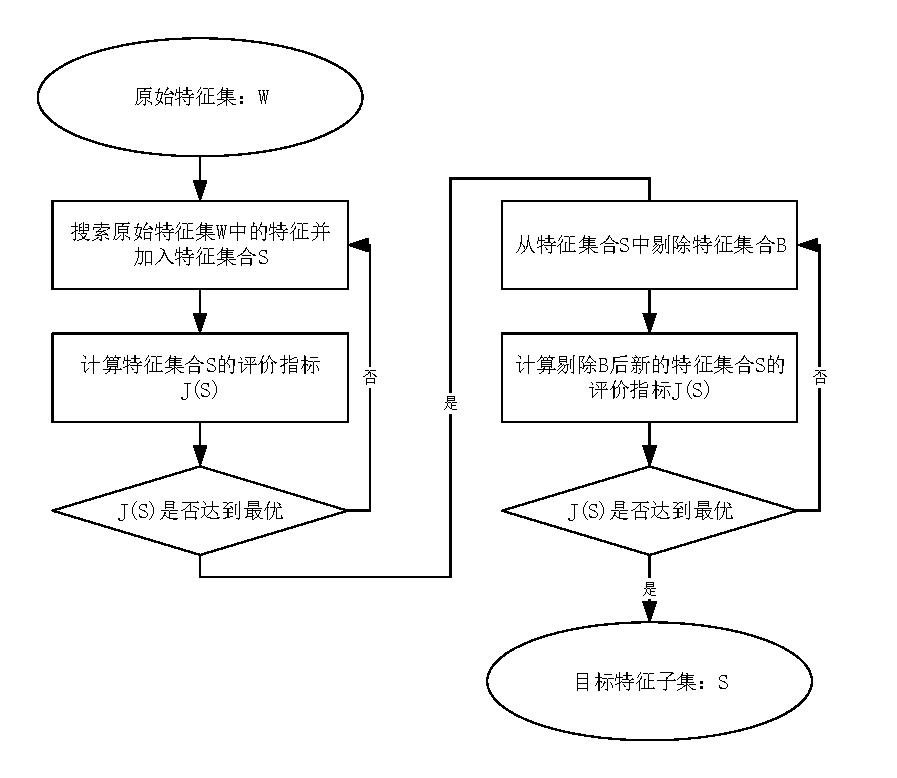
\includegraphics[height=10cm]{myfigures/sffs_feature_select}
    \caption{SFFS特征选择算法流程图}
    \label{fig:sffs_feature_select}
\end{figure}

\subsection{基于情感对的二分类模型}
\label{ssec:emo_pair_bi_cls}

当我们得到每个情感对相关的声学特征集后,下面的任务就是为每个情感对训练二分类器。二分类器的算法有很多种,在论文中我们采用了两种简单的分类器模型:支持向量机(Support Vector Machine, SVM)~\cite{Burges2008A}和贝叶斯逻辑回归(Bayesian Logistic Regression, BLR)~\cite{Genkin2007Large}。

SVM是一种二分类模型,它的基本原理是在特征空间中寻找使数据点的间隔最大化的分类超平面。理想情况下,所有的训练样本都是线性可分的,SVM则可以找到一个完美的分类面将两类数据区分。但大多数情况下,训练样本并不是线性可分的,所以需要其他的一些方法来保证SVM能够正常工作。一般有两种方法:软间隔(Soft Margin)和核函数(Kernel Function)。软间隔通过在目标函数中引入松弛变量,从而解决由于个别离群点导致得到的分类超平面偏移到不好的位置的问题。核函数则是通过将原始数据点映射到更高维的特征空间,使得在低维空间线性不可分的数据点在高维空间变得线性可分。

 BLR是一种假设变量服从某种分布的逻辑回归(Logistic Regression)模型。首先,让我们先回顾下普通的逻辑回归模型,假设我们有特征向量$\phi$,两个类别$C_1$和$C_2$,我们需要建模后验概率$P(C_i|\phi)(i=1,2)$,逻辑回归模型采用下面的公式来建模:
 \begin{equation}
\label{equ:lagrange_multiplier}
    P(C_i|\phi) = \sigma(w^T\phi)
\end{equation}
其中$w$代表我们需要学习的参数,$\sigma$代表sigmoid函数。通过最大似然的算法就可以学习到参数的值。普通的逻辑回归模型都不假设后验概率服从某种分布,这也导致在拟合参数时和训练数据是强相关的,容易出现过拟合的情况。而贝叶斯方法通常都会假设后验概率的分布情况,训练数据通常都是用来估计概率分布的参数,然后再用概率分布去估计类别的概率,这样可以减少过拟合的情况,但是如果数据不服从假设的分布,也会导致训练结果变差。BLR的目的就是将贝叶斯方法的概率分布假设引入逻辑回归的参数估计中,具体来说就是在模型训练时不再精确地估计参数$w$,而是假设参数$w$服从某种分布,然后转而去估计这种分布的参数,这可以通过拉普拉斯近似的方法来实现,具体的细节可以参考~\cite{Genkin2007Large}。通过这种方式就可以有效的避免过拟合的出现,尤其是在训练数据比较少的情况下也能取得较好的结果。

\section{决策融合}
\label{sec:decision_fusion}
在前面一节,我们已经为所有的情感对选择了相关的特征集,并且得到了二分类结果,但我们的目标是只得到唯一的情感类别,所有还需要一个步骤来将这些情感对的结果进行汇总,也就是决策融合~\cite{Dasarathy1994Decision}。决策融合的算法最早出现在集成学习(Ensemble Learning)领域,因为集成学习通常需要训练多个模型,然后通过决策融合将所有模型的结果整合到一起。决策融合大致可以分为两种:训练型和非训练型。训练型的决策融合就是需要通过训练来建立所有模型的结果和最终结果之间的映射关系,非训练型的决策融合则是通过某些代数规则来将所有模型的结果映射到最终结果。下面会介绍本文中采用的两种决策融合的方法:基于投票的决策融合和基于情感空间的贝叶斯决策融合。

\subsection{基于投票的决策融合}
\label{ssec:voting_decision_fusion}
每一个情感对包含两种情感,二分类器可以得到这两种情感中的一种。假设我们需要识别$M$种情感,则一共可以组成$C_M^2 = \frac{M \times (M - 1)}{2}$个情感对,同样我们也会得到这么多的二分类结果。在所有的二分类结果中,每一种情感出现的次数最多为$M-1$次。基于投票的决策融合就是将所有二分类结果中出现次数最多的那个情感判定为最终的识别结果,因为通常出现次数多代表语音中包含这种情感的信息最多,这属于一种无需训练的决策融合方法。下面是算法描述:

\begin{algorithm}[htb]
    \caption{投票决策算法}
    \label{alg:voting}
    
    \begin{algorithmic}[1]
        \Require %算法的输入, \hspace*{0.02in}用来控制位置,同时利用 \\ 进行换行
            \Statex $M$: 情感类别的数量 
            \Statex $E = \{e_i, i=1,2,...,M\}$: 情感类别的集合
            \Statex $R = \{r_{e_ie_j}|e_i \neq e_j; r_{e_ie_j}, e_i, e_j \in E\}$: 情感对的二分类结果

        \Ensure %算法的结果输出
            \Statex $f$: 最终识别出的情感类别

        \Statex
        \State  计算$R$中不同情感类别出现的次数$N_e = \{n_{e_i}|e_i \in R\}$ % \State 后写一般语句
        \State  选出$N_e$中次数最多的情感类别,构成候选情感类别集合$C_{max} = \mathop{argmax}\limits_{e_i}(Ne) = \{c_k|c_k \in E; k = 1,2,...K\}$~~~~~//其中$K$代表候选集合中情感类别的数量
        \State  $f := c_1$
       \If{$K > 1$} % If 语句,需要和EndIf对应
         \For{$k=2$ to $K$}
                \State $f := r_{fc_k}$~~~~//查看候选集合中两个情感的二分类结果,保留胜出的情感类别
            \EndFor
       \EndIf
        \State \Return $f$
    \end{algorithmic}
\end{algorithm}

投票决策是选取票数最多的情感类别作为最终的结果,但可能会存在多个情感类别具有相同最多票数的情况。在本文采用投票决策算法中,会将所有最大票数的情感类别放入一个候选集合中,然后依次比较该候选集中两个情感所在情感对的二分类结果,保留胜出的那个情感类别,最后将会只剩下唯一的一种情感类别。下面我们将作出形式化的证明:

\begin{proposition}
    投票决策算法在二分类结果正确的情况下一定可以得到正确的情感类别
\end{proposition}
\begin{proof}
    采用和算法~\ref{alg:voting}相同的符号表示,假设$e_i$是目标情感,则可以得到下面的证明过程:
    % \begin{equation*}
    \[
        \begin{aligned}
            R \quad is \quad correct &\Rightarrow n_{e_i} = M - 1 \\
            &\Rightarrow n_{e_j} < M - 1, e_j \in E - \{e_i\} \\
            &\Rightarrow C_{max} = \{e_i\} \\
            &\Rightarrow f = e_i
        \end{aligned}
    \]
    % \end{equation*}
\end{proof}

从证明中可以看出当二分类结果是正确的时候,投票决策算法一定可以得到正确的情感类别,但通常我们无法保证所有二分类器的结果都是正确的,这会导致一些情感的票数相同。尽管在算法~\ref{alg:voting}中我们采取了一些策略保证最后可以得到唯一的情感,但是如果同票的几种情感的二分类结果间的胜出关系出现闭环,我们的投票策略同样无法保证得到的一定是最好的识别结果。比如,假设有三种同票的情感$e_1$,$e_2$和$e_3$,$r_{e_1e_2}=e_1$代表在$e_1$和$e_2$组成的情感对二分类结果中,$e_1$的概率更高。如果出现$r_{e_1e_2}=e_1$,$r_{e_2e_3}=e_2$,$r_{e_1e_3}=e_3$这种情况,投票策略将无法做出有效的判决。此外,投票策略在判断最终的情感类别时是通过二分类器的结果决策,也就是说只有包含目标情感的那些二分类器才对最终的结果有好的影响,而其他二分类器的结果都不会对识别出正确的情感有好的影响。

\subsection{基于情感空间的贝叶斯决策融合}
\label{emo_space_decision_fusion}
鉴于上一节提到的基于投票的决策融合方式存在的问题,我们又提出了一种新的基于情感空间模型~\cite{Cowie2002Emotion}的贝叶斯决策融合来避免这些问题。我们在\ref{ssec:continuous_space}节提到过关于维度情感空间的定义,心理学上将情感通过一个笛卡尔空间坐标系来表示,其中每一个坐标轴都表示一种心理学属性,而不同的情感类别会被映射到空间中不同的位置。常用的情感空间模型有二维情感空间(激活度-效价)和三维情感空间(激活度-效价-支配力)。这里采用三维情感空间模型来描述。假设当前需要识别4种情感:高兴,悲伤,愤怒和中性,这些情感在维度情感空间中的分布大致如图\ref{fig:emo_space_distance}所示。

\begin{figure}[htb] % use float package if you want it here
    \centering
    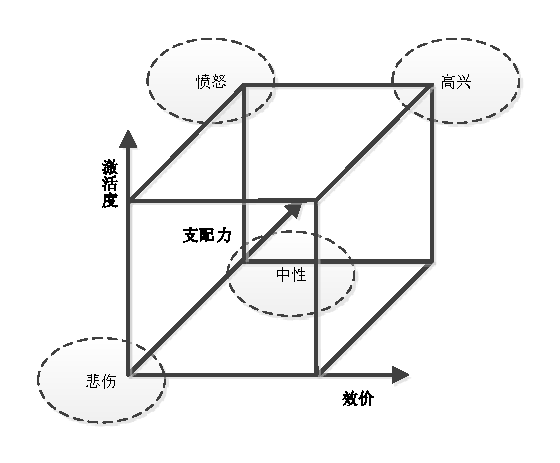
\includegraphics[height=10cm]{myfigures/emo_space_distance}
    \caption{情感空间模型中不同情感的位置}
    \label{fig:emo_space_distance}
\end{figure}

从图中我们可以看出不同的情感类别之间的距离并不相同,例如高兴和愤怒的距离明显比高兴和悲伤的距离要小,而这种情感类别之间的距离恰好反映了它们在情感体现与表征上的相似程度。回想一下日常生活中,当我们高兴地说话和愤怒地说话时,通常语气都比较急促,声音都比较大,但是当我们悲伤地说话时,声音一般都会比较缓慢而低沉。投票决策有个问题就是不包含目标情感的情感对的二分类结果对最后的决策并没有贡献,但现在有了维度情感空间的这种信息,我们可以认为这些不包含目标情感的情感对的二分类结果对最后的决策也是有帮助的。假设目标情感是高兴,对于愤怒-悲伤这个情感对来说,二分类结果是愤怒就更加支持最终的情感类别是高兴,是悲伤的话就更不支持最终的情感类别是高兴,所以二分类结果是愤怒的可能性会更大。这样的支持关系对其他的情感也是适用的。所以如果这种信息能够被有效地运用在决策融合当中,是有助于我们更好地判断最终情感类别的。

对于这种支持关系,需要通过一种数学模型来对其进行量化表示,最为自然的就是想到贝叶斯概率模型,因为这种支持关系可以通过条件概率来建模。假设需要识别的情感类别集合为$E=\{e_i|i=1, 2,...,M\}$,情感对的所有二分类结果为$R = \{r_{e_ie_j}|e_i \neq e_j; r_{e_ie_j}, e_i, e_j \in E\}$。上面关于目标情感为高兴时,对愤怒-悲伤情感对的二分类结果影响程度的例子,通过概率的形式可以表示如下(H:高兴,A:愤怒,S:悲伤):
\begin{equation}
\label{equ:decision_nb_1}
    P(r_{A\_S}=A|H) > P(r_{A\_S}=S|H)
\end{equation}
基于贝叶斯定理,高兴和愤怒-悲伤情感对的二分类结果之间的关系可以被转换为下面的表示:
\begin{equation}
\label{equ:decision_nb_2}
    P(H|r_{A\_S}) = \frac{P(r_{A\_S}|H)P(H)}{P(r_{A\_S})}
\end{equation}
\begin{equation}
\label{equ:decision_nb_3}
    P(H|r_{A\_S}) \propto P(r_{A\_S}|H)
\end{equation}
当$P(H)$和$P(r_{A\_S}$都是先验概率时,通过公式\ref{equ:decision_nb_1}和公式\ref{equ:decision_nb_3},我们可以推导出公式\ref{equ:decision_nb_4}:
\begin{equation}
\label{equ:decision_nb_4}
    P(H|r_{A\_S}=A) > P(H|r_{A\_S}=S)
\end{equation}

为了将这种概率关系推广到所有情感对二分类结果的决策融合中,我们通过朴素贝叶斯分类器来建模。目标情感$e_i$的后验概率可以表示如下:
\begin{equation}
\label{equ:decision_nb_5}
    P(e_i|R) = \frac{P(R|e_i)P(e_i)}{P(R)}
\end{equation}
其中,$P(e_i|R)$代表给定所有的二分类结果R后,得到情感$e_i$的条件概率;$P(R|e_i)$代表已知目标情感是$e_i$,不同二分类器结果的条件概率;$P(e_i)$和$P(R)$分别代表目标情感和二分类结果的先验概率。由于不同情感对的二分器分别是在不同的特征集上训练,所以我们可以假设这些二分类器的输出都是条件独立的。这个假设在数学上并不严谨,但这对我们最终的推导结果并没有太大的影响,因为最终的结果只是一个比例关系。基于这种假设,公式\ref{equ:decision_nb_5}可以被表示为下面的公式\ref{equ:decision_nb_6}:
\begin{equation}
\label{equ:decision_nb_6}
    P(e_i|R) = \frac{\prod_{r_{e_je_k} \in R}P(r_{e_je_k}|e_i)P(e_i)}{P(R)}
\end{equation}
类似公式\ref{equ:decision_nb_2}到公式\ref{equ:decision_nb_3}的转换,我们也可以通过公式\ref{equ:decision_nb_6}推导出下面关于目标情感和情感对二分类结果之间的关系:
\begin{equation}
\label{equ:decision_nb_7}
    P(e_i|R) \propto \prod_{r_{e_je_k} \in R}P(r_{e_je_k}|e_i)
\end{equation}

通过上面的概率推导,我们能够得出这样的结论:当采用朴素贝叶斯分类器作决策融合时,不同情感在维度情感空间中的距离信息能够被引入进来。这使得不仅包含目标情感的情感对的二分类结果对最终的决策有影响,而且不包含目标情感的情感对的二分类结果也可以对最终决策提供辅助信息,进而提升情感识别的准确率。此外,基于贝叶斯的决策融合不存在投票决策中存在的同票问题。在模型训练时,我们将首先得到情感对的二分类结果,再通过朴素贝叶斯分类器建立这些二分类结果和最终目标情感的映射关系。

\section{实验结果及分析}
\label{sec:experiment}

前面几节详细的介绍了我们提出的基于情感对的特征选择和不同的决策融合方法,这两部分共同构成了整个语音情感识别系统,下面我们将通过实验来对比基于情感对的语音情感识别框架和其他语音情感识别框架之间的识别效果。

\subsection{实验设置}
\label{ssec:experiment_setup}

\subsubsection{情感语音数据库}
\label{sssec:speech_database}

在本章中,所有的实验都是基于IEMOCAP情感语音数据~\cite{Busso2008IEMOCAP}库来进行的。在\ref{sec:emo_speech_database}节,我们已经对IEMOCAP数据库做了一个简要的介绍。这是一个人类情感交流相关的数据库,主要被设计用于多模态情感表现研究,包括肢体动作、音频和视频,一共有5个部分,每个部分包括10个主题,总共有接近12个小时的数据,语言为英语。每一个部分包含一个不同的对话场景,会有一个男演员和一个女演员分别表演规定好的剧本,以及在一个对话中诱发情感,所有的过程都是在专业的录音棚中进行。至少三个母语为英语的标记员对同一句话标记情感类别,包括高兴、悲伤、中性、愤怒、惊讶、激动、沮丧、厌恶、恐惧这些情感标签。除了离散的情感标签,标记员还需要通过FeelTrace软件标注每个句子在维度情感空间的心理学属性。这个数据库被许多的研究工作采用,因此可以用来与别人的实验结果作对比。在本文中,我们将只采用其中的语音数据,并且只使用那些三个标记员中至少有两个标记为同一种情感标签的句子,这样的句子表达的情感更为清晰。此外,由于数据库中不同情感标签的句子数量不相同,尤其一些情感的句子数量和其他情感相差太多,所以在我们的研究中将只针对愤怒、高兴、悲伤和中性这四种情感。因为这几种情感的语音数据相对较多,同时这也是大多数使用这个数据库的研究所采用的配置。下面的表格\ref{tab:emo_sample_num}列举了属于不同的情感的句子数量。

\begin{table}[htb]
\centering
\begin{minipage}[htb]{0.8\linewidth} % 如果想在表格中使用脚注,minipage是个不错的办法
\caption{IEMOCAP数据库~\cite{Busso2008IEMOCAP}中不同情感的句子数量}
\label{tab:emo_sample_num}
    % \begin{tabular}{p{6cm}<{\centering} p{6cm}<{\centering}}
    \begin{tabularx}{\linewidth}{X<{\centering} X<{\centering} X<{\centering} X<{\centering} X<{\centering}}
        \toprule[1.5pt]
        中性 & 愤怒 & 高兴 & 悲伤 & 总计 \\
        \midrule[1pt]
        1708 & 1103 & 595 & 1084 & 4490 \\
        \bottomrule[1.5pt]
    \end{tabularx}
\end{minipage}
\end{table}

本文主要针对于说话人无关的语音情感识别,在实验中我们将不同说话人的数据区分开。数据库由10个演员录制,所以分为10份语音数据,其中1个人的数据作为测试集,1个人的数据作为验证集,剩下8个人的数据作为训练集,并且会采用交叉验证(10-Fold Cross Validation),将10个演员的数据依次作为测试集,最后的准确率是所有测试结果的平均值。交叉验证的方法可以在统计学意义上保证实验结果的有效性和可泛化性,使得模型不会因为数据的改变而产生较大偏差。上述实验设置与现有研究~\cite{Lee2009Emotion}的设置相同。

\subsubsection{声学特征集合}
\label{sssec:acoustic_feature_set}

表格\ref{tab:acoustic_feature}展示了我们在实验中所采用的声学特征列表和使用的统计函数,这个特征集合被用在Interspeech2009语音情感识别比赛~\cite{Schuller2009The}上,因此被许多研究作为基准特征集来使用。我们采用OpenSmile工具~\cite{Eyben2010Opensmile}包来抽取这些声学特征,特征集合中有16个低级描述子(Low Level Descriptors),包括韵律学特征,谱相关的特征和声音质量特征。由于这些特征都是基于语音帧来抽取,所以将采用统计函数来得到整个句子的特征表示,最终对于每一个句子将会得到384个特征。后面的所有实验都是基于这个特征集合进行的。对于使用全局特征的的模型将会输入所有的384维特征值。而对于选择特征子集的模型将会从这个特征集中选择出最符合当前任务的特征子集,通常会将每个特征子集中特征的数量控制在40-60个。这样设置是为了和之前相关的工作~\cite{Lee2009Emotion}保持一致,从而便于比较。

\begin{table}[htb]
\centering
\begin{minipage}[htb]{0.8\linewidth} % 如果想在表格中使用脚注,minipage是个不错的办法
\caption{声学特征列表及其统计函数}
\label{tab:acoustic_feature}
    % \begin{tabular}{p{6cm}<{\centering} p{6cm}<{\centering}}
    \begin{tabularx}{\linewidth}{X<{\centering} X<{\centering}}
        \toprule[1.5pt]
        原始特征类型 & 统计函数 \\
        \midrule[1pt]
        基频(f0) & 均值,标准差,峰值 \\
        均方根能量(rms) & 斜率,最小值,最大值 \\
        过零率(zcr) & 相对位置,范围 \\
        信噪比(hnr) & 二次线性回归系数 \\
        梅尔频率倒谱系数(1-12 mfcc) & 线性回归均方差 \\
        \bottomrule[1.5pt]
    \end{tabularx}
\end{minipage}
\end{table}

在得到每个句子的特征值后,我们采用z-normalization对每一维特征进行正则化,具体做法是计算训练集所有中性样本中每一维特征的均值和标准差,然后将所有样本的对应特征减均值除标准差。这里我们做了一个假设:所有说话人在中性语音上的差异不是很大。通过这种正则化后,可以比较好的消除掉不同说话人的声音特点。

\subsection{实验结果}
\label{ssec:experiment_result}

实验结果主要可以分为两个部分,第一部分主要比较了基于情感对的语音情感识别框架和其他的方法的准确率,并且分析了不同情感的混淆矩阵(Confusion Matrix)的变化;第二部分主要展示当目标情感不同时,所有情感对的二分类结果的分布直方图,从而验证维度情感空间中不同情感的距离信息是能够反应不同情感的相似程度,并且这种相似是可以在模型输出中观测到的。

\subsubsection{准确率对比}
\label{sssec:emo_pair_acc_compare}

首先我们将对比不同方法的加权准确率(Weighted Accuracy, WA)和不加权准确率(Unweighted Accuracy, UA),其中WA的计算方式是用测试集中正确分类的样本数量除以总的样本数量,能够反映分类器模型的整体效果;UA的计算方式则首先计算出不同情感类别的准确率,然后对所有情感类别取平均值,这样的得到的准确率可以反映模型对于不同的情感的识别是否均衡。这两个评价指标在之前许多情感识别相关的比赛中被使用,可以方便和其他人的工作作对比。

在下面的表\ref{tab:acc_emo_pair}中,我们展示了多种语音情感识别方法在上面的实验设置中得到的WA和UA。其中,“全局特征选取”代表对于将语音情感识别建模为多分类任务,为所有的情感选取相同的特征集合;“决策树分层特征选取”代表采用基于决策树的语音情感识别框架,在不同树节点选取不同的特征子集;“情感对特征选取”代表采用基于情感对的语音情感识别框架,为不同的情感对选取不同的特征子集;“+”后面是使用的分类器,“SVM”代表支持向量机,“BLR”代表贝叶斯逻辑回归;对于情感对的方法,还列出了不同的决策融合方法,“投票决策”代表采用投票的决策融合,“贝叶斯决策”代表采用考虑情感空间信息的贝叶斯决策融合。从实验结果中可以看到,基于情感对的框架在不同的分类器上都可以取得比其他框架更好的WA和UA。此外,在情感对的框架中,当我们采用贝叶斯决策方法时,可以取得比采用投票方法更好的效果,这是因为引入不同情感在情感空间中的距离信息有助于在最后决策时更好的判断最终的情感类别。

\begin{table}[htb]
\centering
\begin{minipage}[htb]{1.0\linewidth} % 如果想在表格中使用脚注,minipage是个不错的办法
\caption{不同方法的准确率}
\label{tab:acc_emo_pair}
    % \begin{tabular}{p{6cm}<{\centering} p{6cm}<{\centering}}
    \begin{tabularx}{\linewidth}{X<{\centering} X<{\centering} X<{\centering}}
        \toprule[1.5pt]
        模型 & WA & UA \\
        \midrule[1pt]
        全局特征选取 + SVM & 52.41\% & 51.02\% \\
        全局特征选取 + BLR & 53.47\% & 53.55\% \\
        决策树分层特征选取 + SVM & 55.98\% & 58.76\% \\
        决策树分层特征选取 + BLR & 56.38\% & 58.46\% \\
        情感对特征选取 + SVM + 投票决策 & 55.53\% & 58.16\% \\
        情感对特征选取 + BLR + 投票决策 & 56.15\% & 58.54\% \\
        情感对特征选取 + SVM + 贝叶斯决策 & 57.23\% & 62.16\% \\
        情感对特征选取 + BLR + 贝叶斯决策 & \textbf{57.85\%} & \textbf{62.54\%} \\
        \bottomrule[1.5pt]
    \end{tabularx}
\end{minipage}
\end{table}

为了进一步分析不同情感的识别率,我们将展示不同的方法得到的混淆矩阵。为了简单起见,我们将只列出当分类器为BLR时的混淆矩阵,因为SVM得到的结果和BLR是相似的,对于情感对的框架,我们也只展示了贝叶斯决策的结果,因为效果更好。下面的表\ref{tab:cm_global}、表\ref{tab:cm_hierarchical}和表\ref{tab:cm_emo_pair}分别是三种不同的框架得到的混淆矩阵,从中我们可以看到基于决策树的框架和基于情感对的框架在所有情感的准确率上都要优于全局选取特征的多分类框架,这证明为不同的情感选取不同的声学特征是有助于提高语音情感识别系统效果的。此外,相对于决策树的框架,我们可以发现情感对的框架在愤怒、高兴、悲伤这三种情感的准确率上都更高,这是因为当我们引入情感空间的距离信息之后,不同情感之间的混淆在决策融合阶段被减轻了。此外,中性情感的准确率并没有发生明显的变化,这可能是因为中性情感在情感空间中和其他情感的距离没有明显的差别,这使得贝叶斯决策并没有产生帮助。这些实验数据证明了我们提出的基于情感对识别框架在非中性情感的识别上是优于基于决策树的框架的。

\begin{table}[htb]
\centering
\begin{minipage}[htb]{0.8\linewidth} % 如果想在表格中使用脚注,minipage是个不错的办法
\caption{混淆矩阵(全局特征选取 + BLR)}
\label{tab:cm_global}
    % \begin{tabular}{p{6cm}<{\centering} p{6cm}<{\centering}}
    \begin{tabularx}{\linewidth}{X|X|X|X|X}
        \toprule[1.5pt]
        \diagbox[width=5em,trim=l]{实际}{预测} & 中性 & 愤怒 & 高兴 & 悲伤 \\
        \midrule[1pt]
        中性 & \textbf{52.41\%} & 7.98\% & 16.31\% & 23.30\% \\
        愤怒 & 17.64\% & \textbf{60.55\%} & 18.32\% & 3.49\% \\
        高兴 & 25.32\% & 24.58\% & \textbf{39.28\%} & 10.82\% \\
        悲伤 & 30.12\% & 2.82\% & 5.10\% & \textbf{61.96\%} \\
        \bottomrule[1.5pt]
    \end{tabularx}
\end{minipage}
\end{table}

\begin{table}[htb]
\centering
\begin{minipage}[htb]{0.8\linewidth} % 如果想在表格中使用脚注,minipage是个不错的办法
\caption{混淆矩阵(决策树分层特征选取 + BLR)}
\label{tab:cm_hierarchical}
    % \begin{tabular}{p{6cm}<{\centering} p{6cm}<{\centering}}
    \begin{tabularx}{\linewidth}{X|X|X|X|X}
        \toprule[1.5pt]
        \diagbox[width=5em,trim=l]{实际}{预测} & 中性 & 愤怒 & 高兴 & 悲伤 \\
        \midrule[1pt]
        中性 & \textbf{54.51\%} & 6.89\% & 15.20\% & 23.40\% \\
        愤怒 & 16.62\% & \textbf{65.40\%} & 15.26\% & 2.72\% \\
        高兴 & 26.13\% & 19.57\% & \textbf{41.72\%} & 12.58\% \\
        悲伤 & 21.70\% & 2.22\% & 3.88\% & \textbf{72.21\%} \\
        \bottomrule[1.5pt]
    \end{tabularx}
\end{minipage}
\end{table}

\begin{table}[htb]
\centering
\begin{minipage}[htb]{0.8\linewidth} % 如果想在表格中使用脚注,minipage是个不错的办法
\caption{混淆矩阵(情感对特征选取 + BLR + 贝叶斯决策)}
\label{tab:cm_emo_pair}
    % \begin{tabular}{p{6cm}<{\centering} p{6cm}<{\centering}}
    \begin{tabularx}{\linewidth}{X|X|X|X|X}
        \toprule[1.5pt]
        \diagbox[width=5em,trim=l]{实际}{预测} & 中性 & 愤怒 & 高兴 & 悲伤 \\
        \midrule[1pt]
        中性 & \textbf{53.98\%} & 6.19\% & 12.39\% & 27.43\% \\
        愤怒 & 15.46\% & \textbf{68.04\%} & 12.37\% & 4.12\% \\
        高兴 & 21.94\% & 15.82\% & \textbf{50.51\%} & 11.73\% \\
        悲伤 & 14.93\% & 1.49\% & 5.97\% & \textbf{77.61\%} \\
        \bottomrule[1.5pt]
    \end{tabularx}
\end{minipage}
\end{table}

\subsubsection{情感对二分类结果统计}
\label{sssec:emo_pair_acc_compare}

尽管在识别准确率上显示出考虑情感空间信息的贝叶斯决策方式能够取得更好的结果,但为了进一步证明情感对的二分类结果是符合我们关于情感空间的距离能够反映相似度的假设,下面的图\ref{fig:histogram_happy}、图\ref{fig:histogram_angry}、图\ref{fig:histogram_sad}、图\ref{fig:histogram_neutral}将分别展示出当目标情感不同时,所有二分类结果中不同情感的统计直方图。直方图的计算过程是找到测试集中特定目标情感的所有句子,把它们输入到所有情感对的二分类器,统计这些二分类结果中每一种情感出现的次数。统计直方图中,横轴代表不同的情感类别,纵轴代表不同情感在基于情感对的二分类情感识别结果中出现的次数占比,更高的比例表示该情感和目标情感的相似度更高。从图中可以看出,这种比例关系的确和情感空间中不同情感的距离是相关的,例如当目标情感是高兴时,愤怒的比例相对于悲伤的比例更高,而情感空间中也是愤怒和高兴地距离比悲伤和高兴的距离更近。这个统计直方图表明我们关于情感空间中的距离信息能够反映情感相似度的假设是正确的。

\begin{figure}[htb] % use float package if you want it here
    \centering
    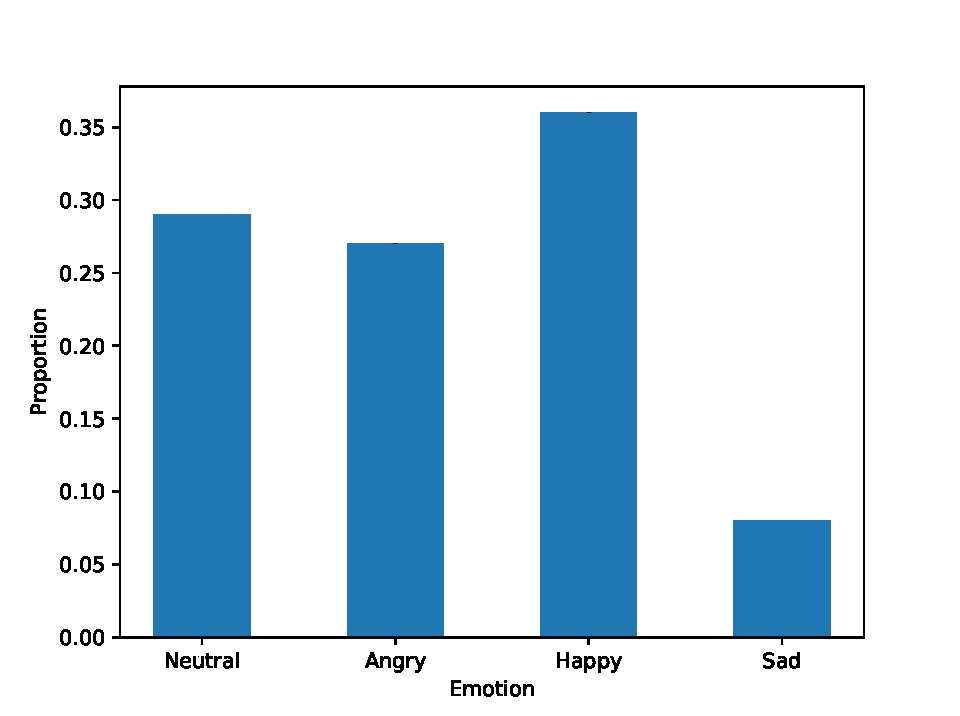
\includegraphics[height=10cm]{myfigures/histogram_happy}
    \caption{二分类结果中不同情感类别的分布直方图(目标情感为高兴)}
    \label{fig:histogram_happy}
\end{figure}

\begin{figure}[htb] % use float package if you want it here
    \centering
    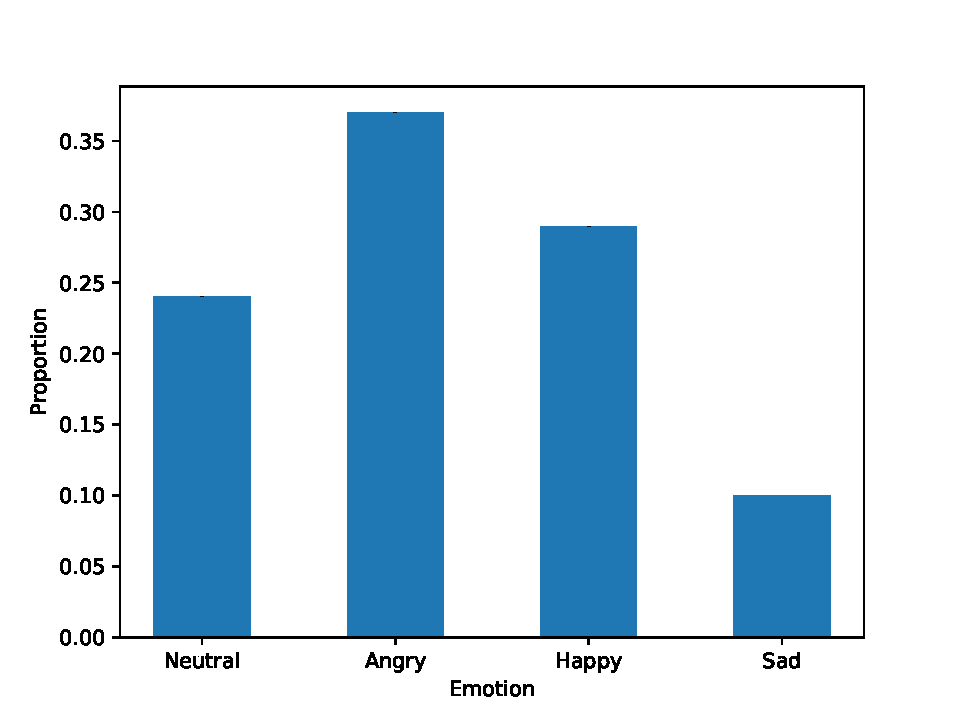
\includegraphics[height=10cm]{myfigures/histogram_angry}
    \caption{二分类结果中不同情感类别的分布直方图(目标情感为愤怒)}
    \label{fig:histogram_angry}
\end{figure}

\begin{figure}[htb] % use float package if you want it here
    \centering
    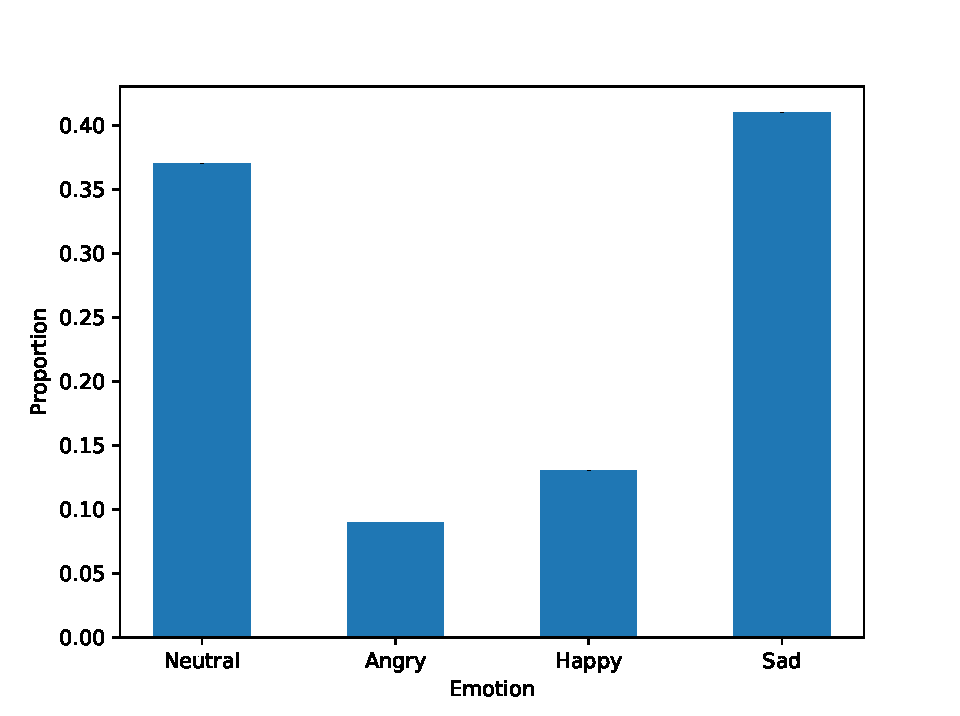
\includegraphics[height=10cm]{myfigures/histogram_sad}
    \caption{二分类结果中不同情感类别的分布直方图(目标情感为悲伤)}
    \label{fig:histogram_sad}
\end{figure}

\begin{figure}[htb] % use float package if you want it here
    \centering
    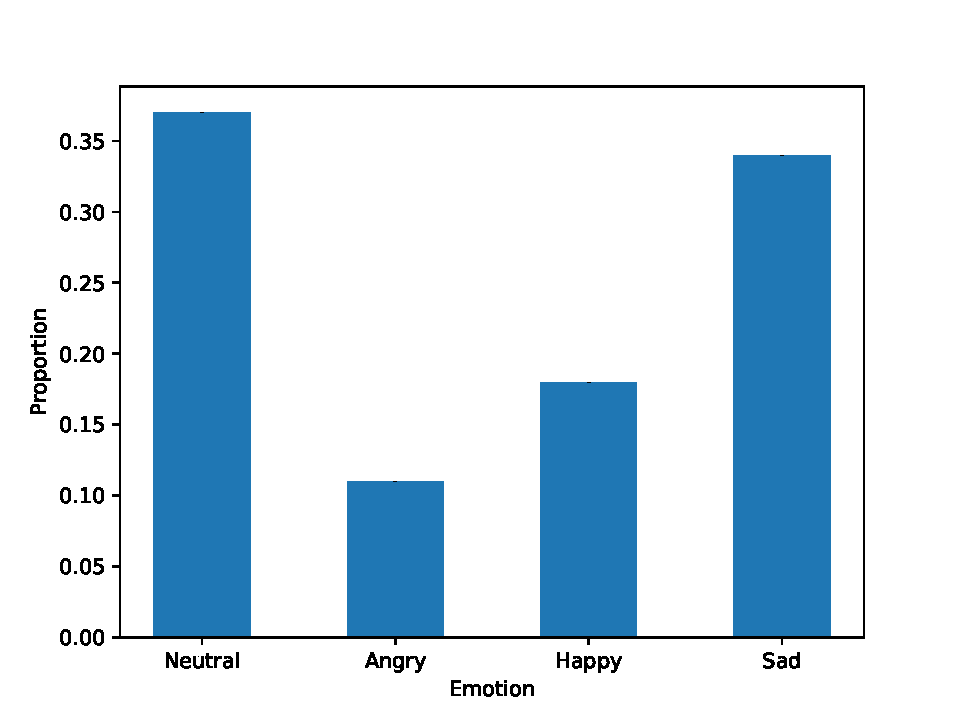
\includegraphics[height=10cm]{myfigures/histogram_neutral}
    \caption{二分类结果中不同情感类别的分布直方图(目标情感为中性)}
    \label{fig:histogram_neutral}
\end{figure}

\section{本章小结}
\label{sec:emo_pair_summary}

本章我们介绍了基于情感对的语音情感识别框架,通过将任意两种不同的情感组成情感对,并且为每一个情感对从一个大的声学特征集合中挑选出适合的特征子集来训练二分类器,最后再将维度情感空间中不同情感的的距离信息加入到决策融合的过程中,从而避免了投票策略中出现的同票问题和无效情感对的问题。在同样的语音情感数据库IEMOCAP以及同样的实验设置下,相比于传统的全局选取特征的多分类框架和基于决策树的识别框架,基于情感对的识别框架加上贝叶斯决策融合可以达到更好的识别准确率,并且当情感类别发生变化时更方便构建识别框架,而不用像基于决策树的框架,需要重新设计决策树结构。同时,由于情感对的二分类器训练相互独立,所以可以并行训练所有二分类器。

    \chapter{基于语谱图的端到端的语音情感识别}
\label{cha:end2end}

\section{本章引论}
\label{sec:end2end_intro}

上一章我们提出的基于情感对的语音情感识别框架取得了不错的效果,但是声学特征仍然采用传统的人工定义的特征,而这些特征无法保证一定能够反映语音中说话人的情感信息。如何从原始语音信号中学习更为有效的特征表示仍然是一个值得关注的问题。此外,当前的情感识别都是对一个完整的句子来判断的,但声学特征通常都是对语音帧抽取的,尽管可以通过对句子中所有语音帧的声学特征计算统计函数来得到整个句子的特征表示,但这样会丢失不同语音帧之间的时序信息。如何在模型中考虑特征间的时序信息同样是一个重要的问题。

近年来,深度学习的技术和工具已经飞速地发展,并且在语音信号处理领域也得到了广泛的应用。在许多的工作中,研究者逐渐开始不使用人工定义的声学特征,转而采用深度神经网络来直接从原始的语音信号上抽取相关的特征表示。这是因为深度神经网络可以从原始信号学习出更加适合任务目标的中间表示,进而使得效果提升,这被称为端到端的系统~\cite{Trigeorgis2016Adieu, Satt2017Efficient}。基于这个原因,本章将构建基于深度神经网络的端到端语音情感识别系统。

本章剩余的部分是这样安排的:首先我们将介绍CNN的结构,以及如何采用CNN从语谱图上抽取情感相关的特征表示,然后介绍RNN的结构,以及如何通过RNN对时间序列进行建模,接下来我们将通过实验对比采用人工定义特征的方法和采用CNN从语谱图抽取的特征的方法在识别效果上的差异,最后总结本章的内容。

\section{基于语谱图的端到端情感识别框架}
\label{sec:cnn_spectrogram_feature}

为了方便神经网络处理,首先会将语音句子切分成更短的等长语音段,并抽取这些语音段的语谱图(Spectrogram),然后通过卷积神经网络(Convolution Neutral Network, CNN)来从语谱图中抽取和情感相关的声学特征,接下来采用循环神经网络(Recurrent Neural Network, RNN)来建模时间序列信息,最终通过全连接神经网络建立输出RNN最后一个时间步的输出和情感类别后验概率之间的映射关系,整个系统的流程如图\ref{fig:end2end_flow}。在预测阶段,会首先计算句子包含的所有等长语音段输入模型后得到的每种情感类别的后验概率,然后对每种情感的后验概率在所有等长语音段上的平均值,平均值最大的情感类别作为模型最终识别出的句子的情感类别。

\begin{figure}[htb] % use float package if you want it here
    \vspace{-0.8cm}  %调整图片与上文的垂直距离
    \setlength{\belowcaptionskip}{0cm}   %调整图片标题与下文距离
    \centering
    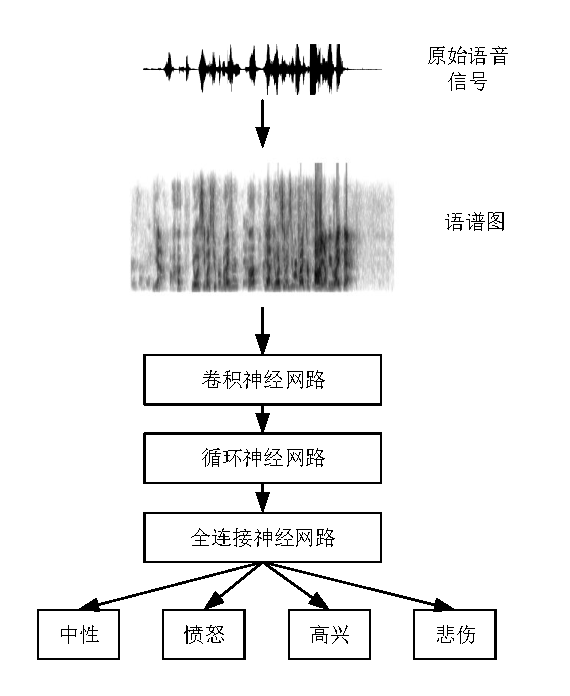
\includegraphics[height=12cm]{myfigures/end2end_flow}
    \caption{基于语谱图的端到端语音情感识别系统流程图}
    \label{fig:end2end_flow}
\end{figure}

\section{基于语谱图的卷积神经网络特征抽取}
\label{sec:cnn_spectrogram_feature}

\subsection{语谱图的定义}
\label{ssec:spectrogram}

语谱图是语音信号的不同频率的能量在时间上的变化,为了方便观测,通常会以图像的方式展示出来。图\ref{fig:spectrogram_example}给出了一张语谱图,其中横轴代表时间,纵轴代表频率,像素点的灰度值代表能量强度,颜色越深代表能量越高。假设原始语音信号为向量$\mathbf{x}$,滑动窗口的长度为$w$,语谱图可以通过下面的公式\ref{equ:spectrogram}计算出来:
\begin{equation}
\label{equ:spectrogram}
    Spectrogram(x, w) = |STFT(x, w)|^2
\end{equation}
其中$STFT(x, w)$代表对滑动窗口内的信号序列进行短时傅里叶变换(Short-Time Fourier Transform, STFT),前后两个窗口之间可以有重叠,每一个窗口经过傅里叶变换后得到的向量即为语谱图中每一个时间点对应的向量。当抽样频率大于语音信号频率的两倍时,根据奈奎斯特定理经过傅里叶变换的信号是能够恢复原始信号的,所以语谱图相对于原始语音信号没有任何信息损失,并且更容易进行频谱上的预处理,例如滤波、去噪等。通常,情感信息主要集中在语音信号的低频区域,所以我们可以采用低通滤波器对语谱图进行预处理,排除高频信息对情感识别的干扰,而原始语音信号做这样的预处理会更麻烦。

\begin{figure}[htb] % use float package if you want it here
    \vspace{-0.8cm}  %调整图片与上文的垂直距离
    \setlength{\abovecaptionskip}{-0.5cm}
    \setlength{\belowcaptionskip}{0cm}   %调整图片标题与下文距离
    \centering
    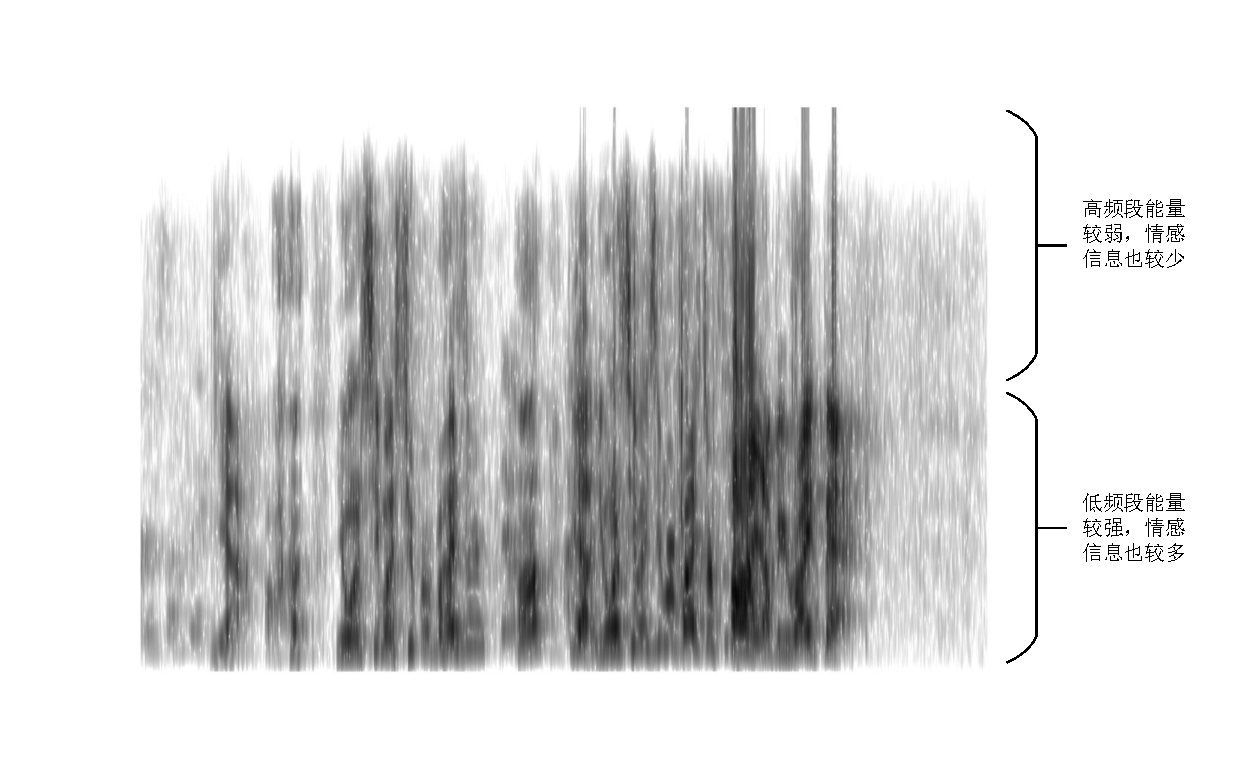
\includegraphics[height=10cm]{myfigures/spectrogram_example}
    \caption{语谱图示例}
    \label{fig:spectrogram_example}
\end{figure}

语谱图在语音信号处理领域的运用十分广泛,通常被用来观测语音信号在频谱上的变化。在语谱图上,我们可以观测到共振峰,信号强度等信息,相比于原始的语音信号,语谱图可以更直观的观测语音在时域和频域上的变化。在本章所构建的端到端的语音情感识别识别系统中,语谱图将作为模型的输入。

\subsection{卷积神经网路}
\label{ssec:cnn}

卷积神经网络(Convolution Neutral Network, CNN)是近年来被广泛使用的一种深度神经网络结构,它实际上可以被认为是将一种神经网络结构进行多份复制,然后将这些复制作用在输入的不同部分。这种网络结构可以处理规模很大的输入,同时又可以保证模型参数的数量保持不变,这使得存储模型所需的空间大大减少。这种重复利用的思想和程序设计中函数的用法很相似,就是编写一个函数的代码,然后在不同的地方调用。

为了方便表述,我们先来看一维的语音信号输入,假设我们的目的是将语音信号进行分类,输入被表示为向量$\mathbf{x}=\{x_0,x_1,...x_8\}$,CNN的单一结构,也被称为卷积核,被表示为$A$,每一个卷积核仅仅作用在一部分输入上,最后的分类输出通过一个全连接层$F$来完成,整个结构如图\ref{fig:cnn_1_layer}所示。

\begin{figure}[htb] % use float package if you want it here
    \vspace{-0.5cm}  %调整图片与上文的垂直距离
    \setlength{\belowcaptionskip}{0cm}   %调整图片标题与下文距离
    \centering
    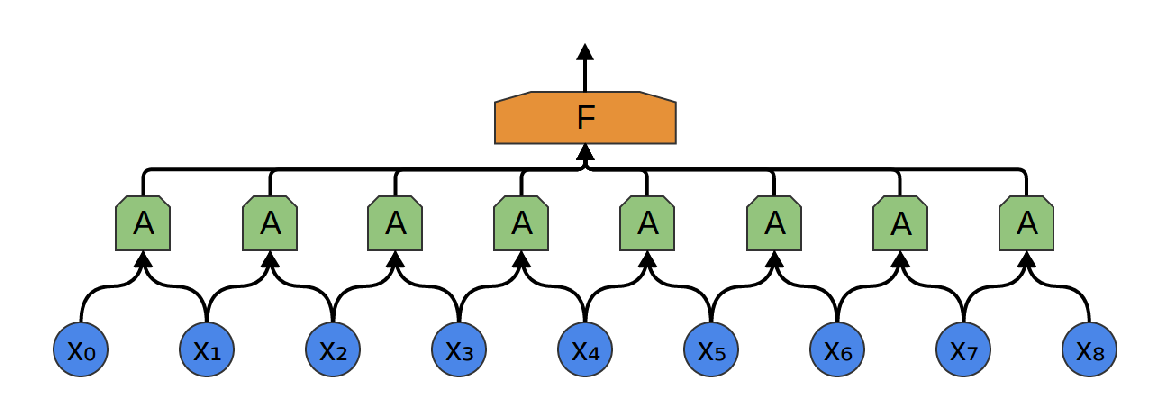
\includegraphics[height=5cm, width=12cm]{myfigures/cnn_1_layer}
    \caption{一维卷积神经网络(单卷积层)}
    \label{fig:cnn_1_layer}
\end{figure}

通常一个CNN网络会有多个卷积核,每一个卷积核代表对一小段输入的特征表示。此外,CNN可以堆叠多层,假设我们有一组新的卷积核$B$,则可以在$A$上面再叠加一层$B$,以此来得到更高级,更抽象的特征,结构如图\ref{fig:cnn_2_layer}所示。

\begin{figure}[htb] % use float package if you want it here
    \vspace{-0.5cm}  %调整图片与上文的垂直距离
    \setlength{\belowcaptionskip}{0cm}   %调整图片标题与下文距离
    \centering
    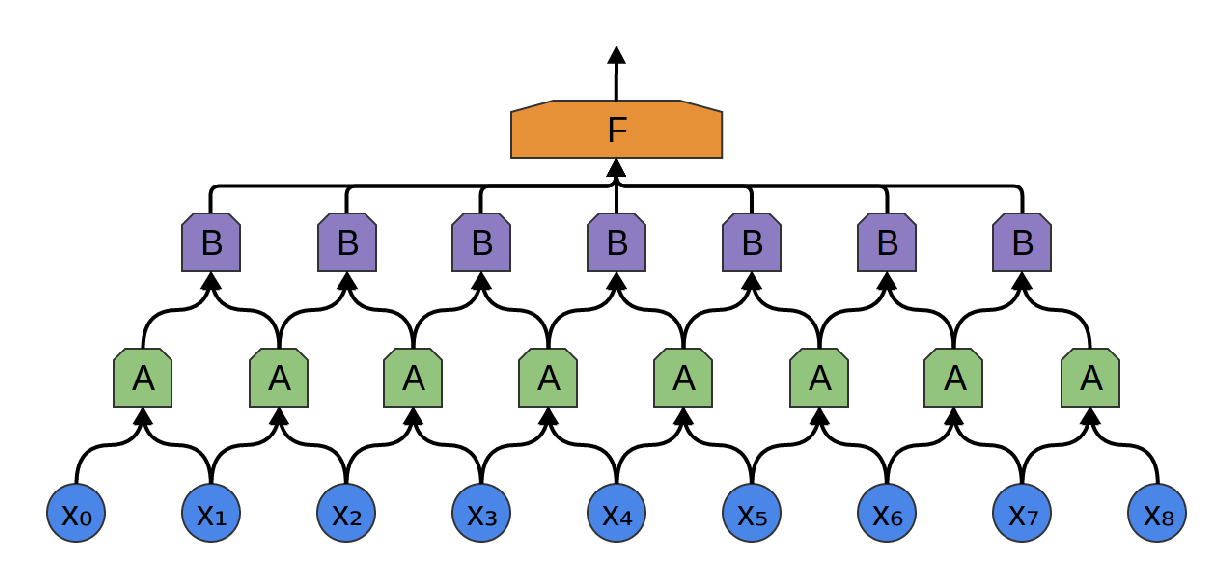
\includegraphics[height=6cm, width=12cm]{myfigures/cnn_2_layer}
    \caption{一维卷积神经网络(双卷积层)}
    \label{fig:cnn_2_layer}
\end{figure}

CNN通常还会在后面加一层池化层(Pooling Layer),目的是通过计算输入特征的统计量来保证不变性,这种不变性包括平移、旋转、尺度的不变性等。此外,还可以对输入进行降维,并且使得网络能够作用在更大的输入段上。最大值池化层(Max-Pooling Layer)是一种被广泛使用的池化层,它的目的是从上一层的每一块输出中的找出最大值,因为通常最大值最能够反映一块输出的特性,图\ref{fig:cnn_layer_pooling}给出了最大值池化层的使用方式。

\begin{figure}[htb] % use float package if you want it here
    \vspace{-0.5cm}  %调整图片与上文的垂直距离
    \setlength{\belowcaptionskip}{0cm}   %调整图片标题与下文距离
    \centering
    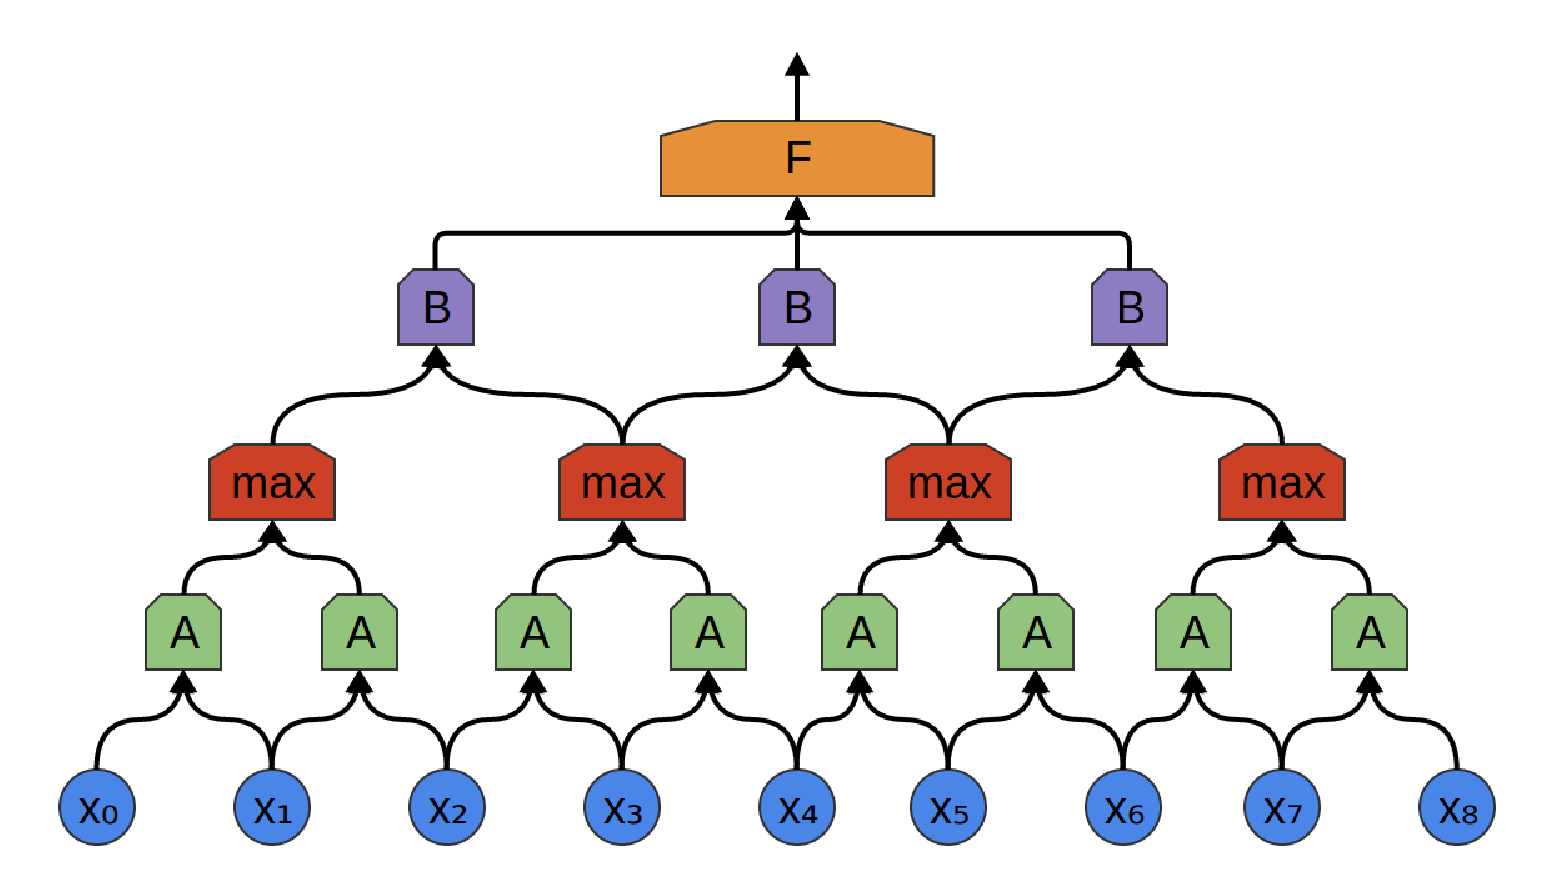
\includegraphics[height=7cm, width=12cm]{myfigures/cnn_layer_pooling}
    \caption{一维卷积神经网络(卷积层+池化层+卷积层)}
    \label{fig:cnn_layer_pooling}
\end{figure}

前面的例子主要介绍的是CNN如何处理一维的输入向量,但语谱图属于二维的输入矩阵,所以我们需要将网络结构扩展到可以处理二维输入矩阵。假设我们有输入矩阵$\mathbf{X}=\{x_{i,j}, i=0,1,...,8; j=0,1,...,8\}$,则CNN的处理将会变成图\ref{fig:cnn_layer_pooling_2dim}的方式。此时,卷积层的卷积核作用在一个二维小块上,然后得到这个小块的特征表示。

\begin{figure}[htb] % use float package if you want it here
    \vspace{-0.5cm}  %调整图片与上文的垂直距离
    \setlength{\belowcaptionskip}{0cm}   %调整图片标题与下文距离
    \centering
    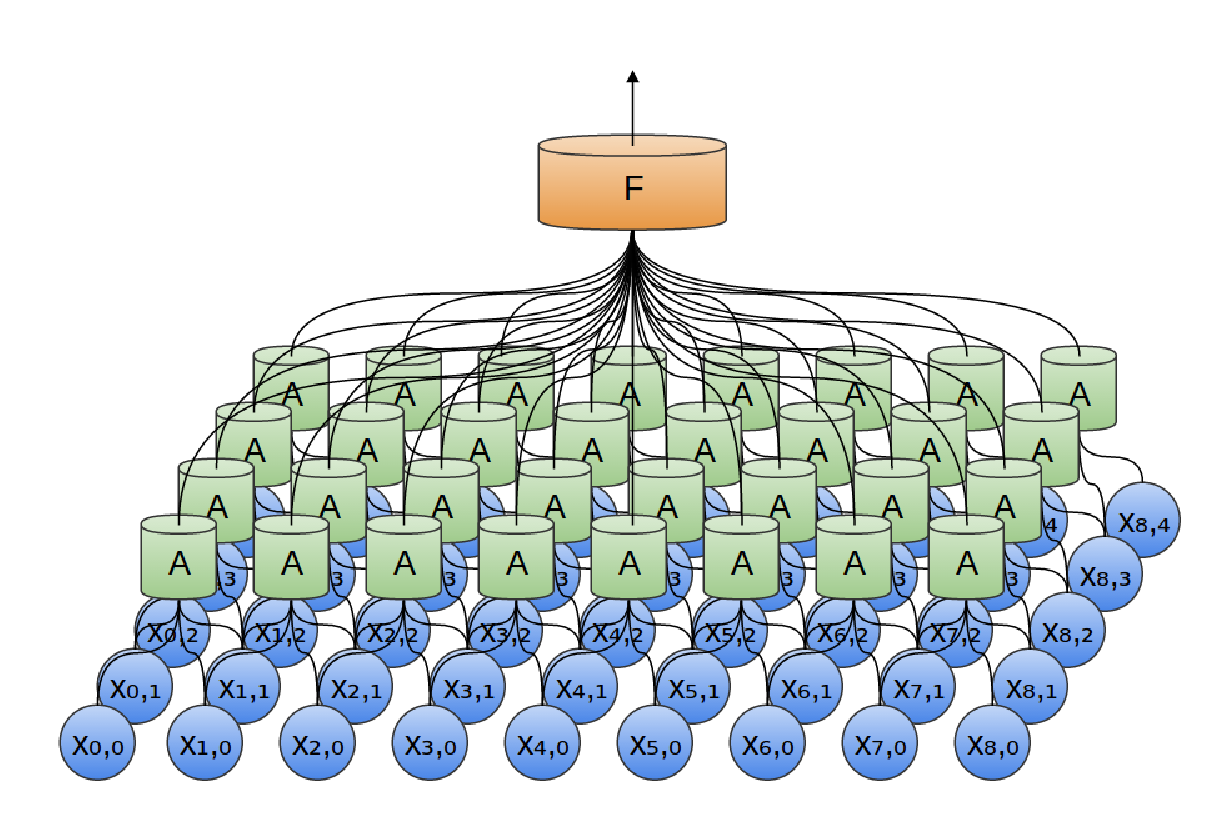
\includegraphics[height=8cm, width=12cm]{myfigures/cnn_layer_pooling_2dim}
    \caption{二维卷积神经网络(卷积层)}
    \label{fig:cnn_layer_pooling_2dim}
\end{figure}

\subsection{基于语谱图的卷积神经网络特征抽取}
\label{ssec:cnn_spectrogram_feature_extract}

CNN最早用在计算机视觉领域,因为它的处理机制和人眼感知图像的机制很类似。语谱图也可以被看做是一张图像,将CNN作为整个深度神经网络中最开始的结构可以起到特征提取的作用。相比于传统的人工定义的声学特征,CNN的训练是取决于最后的分类目标的,所以可以通过CNN得到更加符合当前任务的特征表示。此外,由于CNN是整个深度神经网络模型的一部分,所以当模型中还存在RNN时,抽取特征时还将会考虑到时序信息。通过CNN将语谱图转化为和情感相关的中间表示,就可以为后面的情感分类提供和情感相关的特征输入,从而替代传统语音情感识别框架中的声学特征。

\section{基于循环神经网络的时间序列建模}
\label{sec:rnn_seq_model}

\subsection{循环神经网络}
\label{ssec:rnn}

传统的全连接神经网络中,所有的输入都是相互独立的,但是一些任务需要建立序列输入的前后元素之间的关系,例如在语言模型中,需要根据前面出现的词对后面的词进行预测。循环神经网络(Recurrent Neural Network, RNN)的目的是对序列信息进行建模,它对于序列中的每一个元素都进行相同的计算,当前的输出不仅跟当前的输入相关,而且和之前的输入也相关。

图\ref{fig:rnn}是一个RNN的示意图。图中$\mathbf{x}=\{x_t, t=0,1,...,N\}$为输入序列,$\mathbf{s}=\{s_t, t=0,1,...,N\}$为隐状态序列,$\mathbf{o}=\{o_t, t=0,1,...,N\}$为输出序列,$(U, W, V)$是RNN的权重矩阵。序列中元素之间的映射关系可以通过下面的公式\ref{equ:rnn_cal_state}和\ref{equ:rnn_cal_output}表示:
\begin{equation}
\label{equ:rnn_cal_state}
    s_t = f(Ux_t + Ws_{t-1})
\end{equation}
\begin{equation}
\label{equ:rnn_cal_output}
    o_t = softmax(Vs_t)
\end{equation}
RNN中的隐藏状态是能够建模序列中前后元素关系的关键,因为当前时刻的隐藏状态$s_t$是和上一时刻的隐藏状态$s_{t-1}$相关的,而当前时刻的输出$o_t$和当前时刻隐藏状态$s_t$相关的,所以这使得当前时刻的输出$o_t$会考虑到之前的输入信息。

\begin{figure}[htb] % use float package if you want it here
    \vspace{-0.8cm}  %调整图片与上文的垂直距离
    \setlength{\belowcaptionskip}{0cm}   %调整图片标题与下文距离
    \centering
    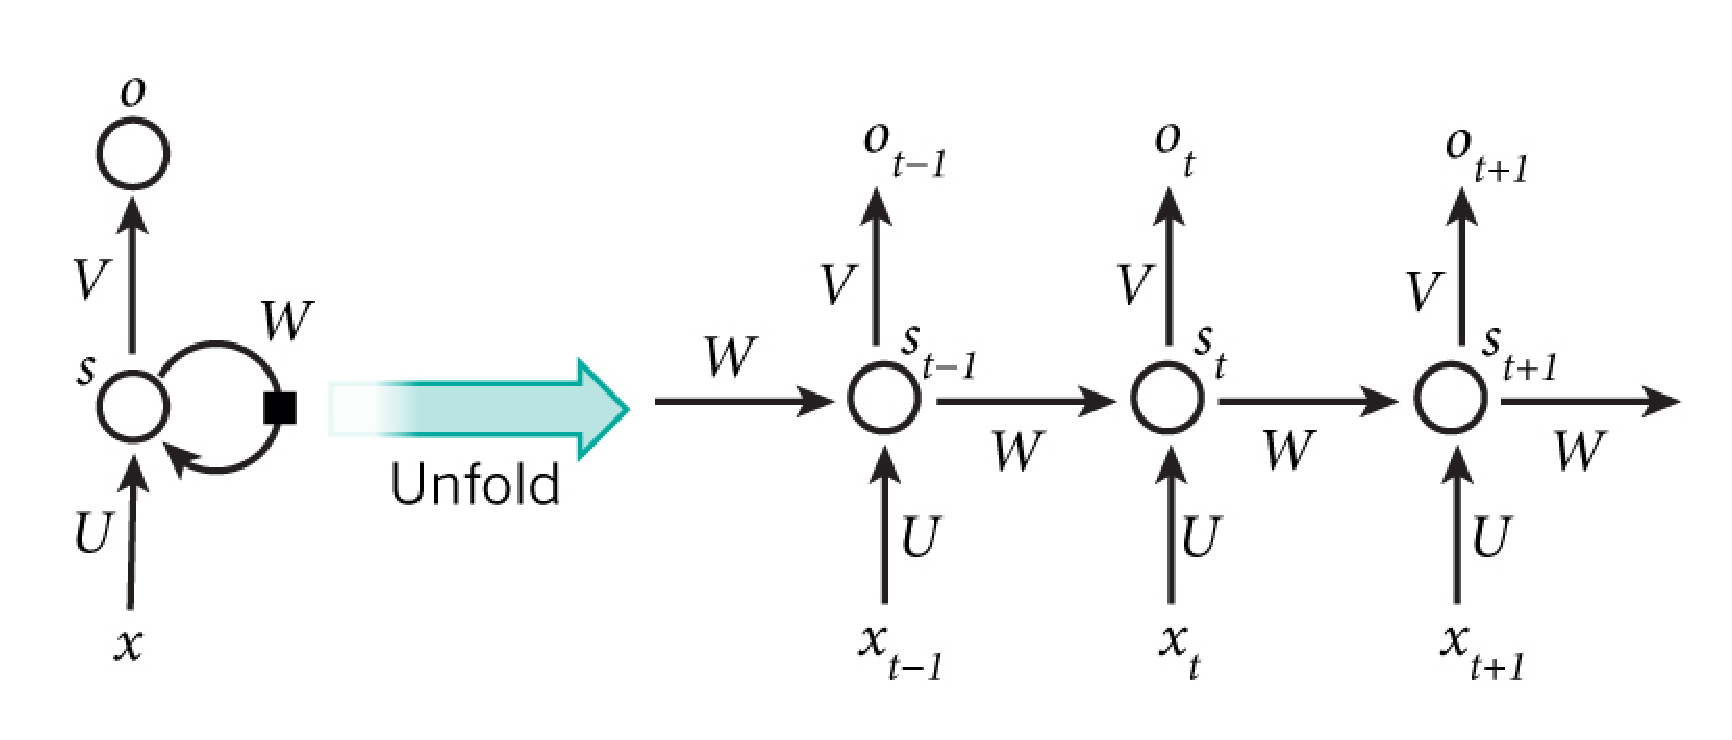
\includegraphics[height=5cm, width=12cm]{myfigures/rnn}
    \caption{循环神经网络}
    \label{fig:rnn}
\end{figure}

对于普通的RNN,当序列时间长度过长时,由于链式乘法规则,会导致出现梯度消失问题,从而使得网络并不能学习到太长时间的信息。这使得一些新的RNN网络结构被提出,例如长短时记忆(Long-Short Term Memory)网络,门循环单元(Gated Recurrent Unit)网络。它们的共同点都是引入了一种门函数(Gated Function)结构,使得网络在建模时序信息时,能够选择记住之前的哪些信息,这样的结构保证网络可以学习到更长时间的序列信息。此外,由于RNN通常只能考虑到从前到后的序列信息,但在许多任务中从后到前的序列信息也是很重要的。因此,一种双向的RNN结构也被提出,具体实现就是正常顺序的序列训练一个RNN,然后将序列逆序后再训练一个RNN,最后将两个RNN的输出拼接在一起,这种RNN结构被称为双向循环神经网络(Bi-Directional Recurrent Neural Network)。

\subsection{基于循环神经网络的时间序列建模}
\label{ssec:rnn_seq_model_detail}

之前我们通过CNN在语谱图上抽取出了相关的特征表示,这种特征表示也是一个时间序列,每一个时间点的输入向量是原始语音信号的频谱经过CNN抽象后得到的特征表示,所以我们可以通过RNN来建立不同时间步之间的时序关系。

由于语音情感识别的目标是对每一个语音段判别情感类别,所以并不需要RNN中所有时间点的输出,仅仅只需要最后一个时间点的输出。当得到RNN的输出后,关于时间序列的信息已经被编码到了当前的表示中,然后再采用全连接神经网络将输出映射到每种情感类别的后验概率,我们就搭建起了整个基于深度神经网络的端到端的语音情感识别系统。


\section{实验结果及分析}
\label{sec:end2end_experiment}

前面几节详细的介绍了基于深度神经网络的端到端的语音情感识别系统,下面我们将通过实验来对比采用人工定义的声学特征和在语谱图上直接抽取特征表示之间的效果差别。

\subsection{实验设置}
\label{ssec:end2end_experiment_setup}

\subsubsection{情感语音数据库}
\label{ssec:end2end_database}

本章所使用的数据库仍然为IEMOCAP情感语音数据库~\cite{Busso2008IEMOCAP},并且也只判别其中的四种情感:中性,愤怒,高兴和悲伤。与上一章不同的是我们将只考虑在对话中诱发的情感语音,不考虑基于特定文本表演的情感语音。因为基于特定文本表演的情感语音包含太强的语言学相关的信息,并不适合分析语音中包含的情感信息。在这章的实验中我们同样会采用交叉验证(5-Fold Cross Validation),但是将数据库按不同的主题分为5个部分,每次都将4个部分作为训练集,另一个部分中一个说话人的数据作为验证集,其他作为测试集,表格\ref{tab:end2end_emo_sample_num}是本实验中不同情感的句子数量:

\begin{table}[htb]
\centering
\begin{minipage}[t]{0.8\linewidth} % 如果想在表格中使用脚注,minipage是个不错的办法
\caption{IEMOCAP数据库中不同情感的句子数量}
\label{tab:end2end_emo_sample_num}
    % \begin{tabular}{p{6cm}<{\centering} p{6cm}<{\centering}}
    \begin{tabularx}{\linewidth}{X<{\centering} X<{\centering} X<{\centering} X<{\centering} X<{\centering}}
        \toprule[1.5pt]
        中性 & 愤怒 & 高兴 & 悲伤 & 总计 \\
        \midrule[1pt]
        1099 & 289 & 284 & 608 & 2280 \\
        \bottomrule[1.5pt]
    \end{tabularx}
\end{minipage}
\end{table}

\subsubsection{语谱图抽取}
\label{ssec:end2end_spectrogram_extract}

IEMOCAP数据库中的语音采用16kHz的采样频率,每个句子的时间长度为1s到30s不等。为了方便神经网络处理,我们首先将这些句子切分成3s长的语音段,不足3s的语音段暂时保留,然后对这些语音段计算语谱图,表格\ref{tab:end2end_spectrogram_setup}是计算语谱图时的参数设置。由于语音中的情感信息主要集中在低频的部分,所以我们只保留0-4kHz的频谱,避免高频段的信息产生干扰。此外,频谱分辨率代表语音帧通过傅里叶变化后得到的向量维度,每一个维度都代表一段频谱的能量。

\begin{table}[htb]
\centering
\begin{minipage}[t]{0.8\linewidth} % 如果想在表格中使用脚注,minipage是个不错的办法
\caption{语谱图计算的参数配置}
\label{tab:end2end_spectrogram_setup}
    % \begin{tabular}{p{6cm}<{\centering} p{6cm}<{\centering}}
    \begin{tabularx}{\linewidth}{X<{\centering} X<{\centering}}
        \toprule[1.5pt]
        参数名称 & 参数值 \\
        \midrule[1pt]
        滑动窗口类型 & 汉明窗(Hamming Window) \\
        滑动窗口长度 & 40ms \\
        滑动窗口偏移 & 10ms \\
        频谱范围 & 0-4kHz \\
        频谱分辨率 & 800 \\
        \bottomrule[1.5pt]
    \end{tabularx}
\end{minipage}
\end{table}

在得到语谱图后,我们通过取对数降低能量表示的取值范围,然后采用z-normalization对所有的样本进行正则化,其中均值和标准差基于语谱图中每一个频率刻度在所有样本中的所有时间的能量。在完成正则化后,还需要将不足3s的语谱图通过在末尾加0补齐到3s,这样就可以保证所有输入样本的长度是相同的。经过上述的处理后,神经网络模型的输入为正则化后的对数频谱分布,其时间长度大小为300(3000ms/10ms$\times$1000),频率尺度大小为400(4kHz/8kHz$\times$800)。

\subsubsection{深度神经网络结构和参数}
\label{ssec:end2end_nn_topology}

在实验中我们采用CNN从语谱图中抽取特征表示,然后使用RNN建模语音信号的时序信息,最后通过全连接网络将RNN最后一个时间步的输出映射到情感类别的后验概率。在尝试了多种的神经网络结构和参数后,图\ref{fig:end2end_nn_topology}是我们当前最好效果的网络结构。其中,卷积层中的参数代表二维卷积核的长和宽;池化层的参数代表缩放的比例;循环神经网络层的参数代表节点的数量和双向网络。此外,由于不同情感的句子数量有所差异,所以在训练时需要对误差函数(Loss Function)乘以权重,这个权重和样本对应的情感类别在数据库中的句子数量成反比,这样可以保证模型不会对样本数量多的情感产生偏好。还有就是我们最后需要得到整个句子的情感类别,所以将会对当前句子切分得到的所有语音段计算不同情感的后验概率,然后将所有语音段的输出结果取平均值,最后将平均值最大的那种情感作为当前句子的情感识别结果。

\begin{figure}[htb] % use float package if you want it here
    \vspace{-0.8cm}  %调整图片与上文的垂直距离
    \setlength{\belowcaptionskip}{0cm}   %调整图片标题与下文距离
    \centering
    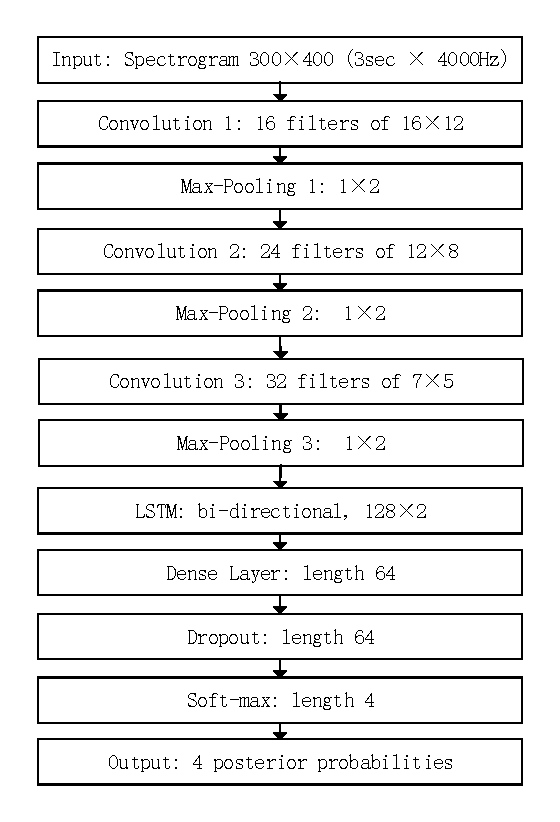
\includegraphics[height=14cm]{myfigures/end2end_nn_topology}
    \caption{深度神经网络结构}
    \label{fig:end2end_nn_topology}
\end{figure}

\subsection{实验结果}
\label{ssec:end2end_experiment_result}

实验结果主要可以分为两个部分,第一部分主要比较了基于人工定义特征的方法和基于语谱图抽取特征的方法之间识别率的差异;第二部分主要通过图像来展示语谱图通过CNN后得到的特征表示,从而进一步证明这种抽取特征的方式能够关注到语谱图中的一些特定模式信息。

\subsubsection{准确率对比}
\label{sssec:end2end_acc_comp}

本次实验的评价指标仍然是加权准确率(Weighted Accuracy, WA)和不加权准确率(Unweighted Accuracy, UA),在下面的表\ref{tab:acc_end2end}中,我们展示了以前采用传统声学特征的工作在IEMOCAP数据集上取得的最好的结果~\cite{Lee2015High}、同样的特征集在我们设计的神经网络模型上的结果、以及语谱图作为输入在我们神经网络模型上的结果。其中,“最佳结果”代表之前在传统声学特征集上取得的最好的结果~\cite{Lee2015High},“神经网络”代表在本章设计的神经网络模型下的结果。将传统特征作为我们设计的神经网络的输入时,每一个时间点的输入会从频谱能量变为传统的声学特征向量。此外,将原始语音信号的作为我们设计的神经网络的输入时,将只对时域进行卷积,因为语音信号是一维的。从实验结果中我们可以看出,当通过深度神经网络直接在语谱图上抽取特征表示时,相比于采用传统声学特征的方法,不仅在WA上取得了明显的提升,而且在UA上也取得了相近的结果。这证明采用神经网络在语谱图上抽取的特征表示相比于传统声学特征更能够反映语音中的情感信息。此外,采用语谱图也可以取得比原始语音信号更好的结果,这是因为我们只保留0-4kHz的频段,而情感信息主要分布在低频段,所以可以过滤到高频段的干扰信息。

\begin{table}[htb]
\centering
\begin{minipage}[t]{1.0\linewidth} % 如果想在表格中使用脚注,minipage是个不错的办法
\caption{不同方法的准确率}
\label{tab:acc_end2end}
    % \begin{tabular}{p{6cm}<{\centering} p{6cm}<{\centering}}
    \begin{tabularx}{\linewidth}{X<{\centering} X<{\centering} X<{\centering}}
        \toprule[1.5pt]
        模型 & WA & UA \\
        \midrule[1pt]
        传统声学特征(最佳结果)~\cite{Lee2015High} & 63.90\% & 62.80\% \\
        传统声学特征(神经网络) & 62.41\% & 60.02\% \\
        原始语音信号(神经网络) & 64.57\% & 61.43\% \\
        语谱图(神经网络) & \textbf{67.30\%} & \textbf{62.00\%} \\
        \bottomrule[1.5pt]
    \end{tabularx}
\end{minipage}
\end{table}

\subsubsection{基于卷积神经网络的特征表示}
\label{sssec:end2end_cnn_feature}

为了进一步观察深度神经网络在语谱图上学习到了什么,我们将最后一层CNN的输出以图像的方式展示出来。下面图\ref{fig:cnn_spectrogram}和图\ref{fig:cnn_activation}展示了一段中性语音的语谱图和最后一层CNN中具有代表性的两个卷积核的输出值,其中横轴代表时间,纵轴代表频率,红色代表高能量,蓝色代表低能量。从图\ref{fig:cnn_activation}中(a)的激活输出中可以观察到这个卷积核学习到了语谱图中垂直方向的模式信息,而从(b)的激活输出中则可以观察到另一个卷积核学习到了语谱图水平方向的模式信息。其他情感的语音在这两个卷积核上也可以观察到这样的现象。这些实验数据表明CNN可以从原始语谱图中捕捉到关于关于语音时域和频域的相关信息。

\begin{figure}[htb] % use float package if you want it here
    \vspace{-0cm}  %调整图片与上文的垂直距离
    \setlength{\belowcaptionskip}{0cm}   %调整图片标题与下文距离
    \centering
    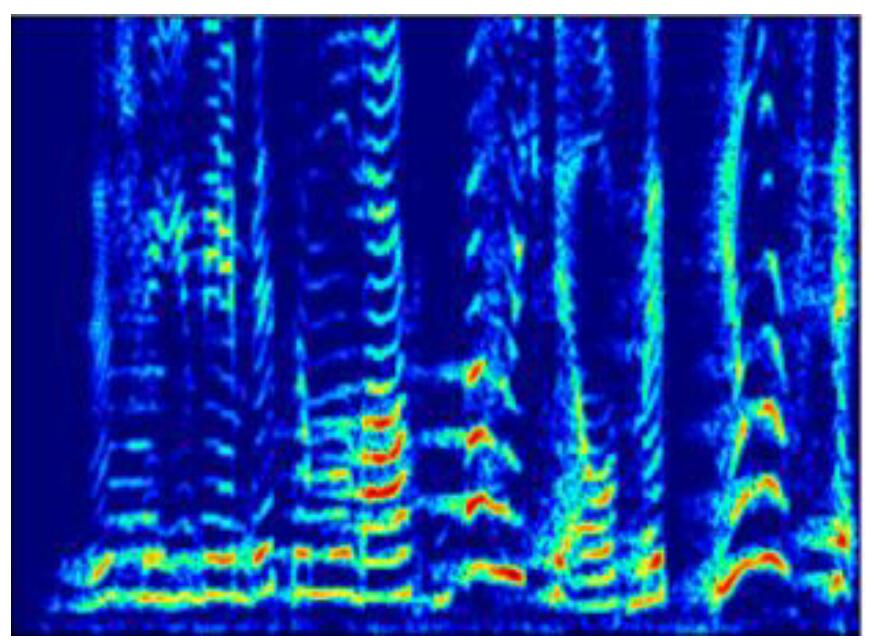
\includegraphics[height=5cm]{myfigures/cnn_spectrogram}
    \caption{原始语谱图}
    \label{fig:cnn_spectrogram}
\end{figure}

\begin{figure}[htb]
    \vspace{-0.8cm}  %调整图片与上文的垂直距离
    \setlength{\belowcaptionskip}{0cm}   %调整图片标题与下文距离
    \begin{minipage}{0.48\textwidth}
        \centering
        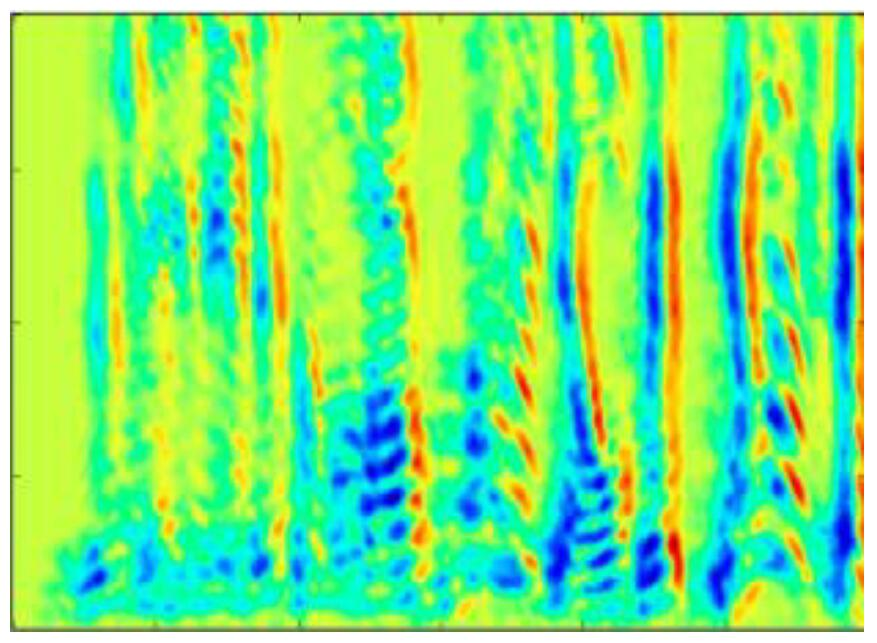
\includegraphics[height=5cm]{myfigures/cnn_vertical}
        \centerline{(a) 垂直方向模式}\medskip
    \end{minipage}\hfill
    \begin{minipage}{0.48\textwidth}
        \centering
        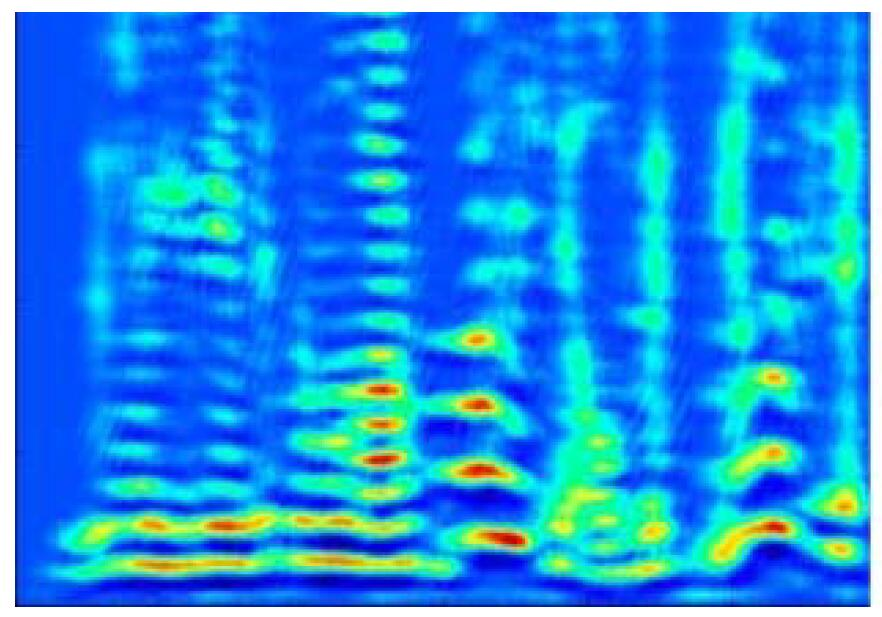
\includegraphics[height=5cm]{myfigures/cnn_horizontal}
        \centerline{(b) 水平方向模式}\medskip
    \end{minipage}
\caption{卷积神经网络中两个卷积核的激活输出}
\label{fig:cnn_activation}
\end{figure}

\section{本章小结}
\label{sec:end2end_summary}

本章我们介绍了基于深度神经网络的端到端的语音情感识别系统,首先通过CNN来直接从语谱图上抽取和情感相关的特征表示,然后采用RNN来建模语音信号的时序关系,最后通过一个全连接神经网络将RNN最后一个时间步的输出映射到不同情感的后验概率。在情感语音数据库IEMOCAP上,相比于之前基于传统声学特征的方法,基于语谱图的端到端系统可以取得更好的识别率。
    \chapter{总结与展望}
\label{cha:summary_prospect}

\section{本文工作总结}
\label{sec:summary}

\section{未来工作展望}
\label{sec:prospect}
    \chapter{总结与展望}
\label{cha:summary_prospect}

\section{本文工作总结}
\label{sec:summary}

随着人机交互日应用的日益普遍,语音情感识别正在逐渐受到更多研究者的的重视。本文主要对语音情感识别中特征抽取和选择的方式进行了研究,包括基于传统声学特征的语音情感识别框架和基于深度学习的端到端的语音情感识别框架。针对现有研究中存在的关于特征选取,特征抽取和变长语音段输入相关的问题,提出了一些有效的解决方案。本文主要的工作可以分为以下几个部分:

\textbf{一、提出一种基于情感对的语音情感识别框架,为不同的情感对选择不同的声学特征,并在最后的决策融合过程中引入心理学的情感空间模型,从而提升了系统的识别率。} 传统的语音情感识别系统通常为所有的情感选取相同的声学特征来完成最后的情感分类,但实验证明不同的情感和不同的声学特征的相关性并不同。针对这一问题,我们将分别为不同的情感对选取不同的特征集合,将原先的多分类问题转变为多个二分类问题,并在最后的决策融合过程中通过贝叶斯分类器引入情感空间的信息。在公开的情感语音数据集IEMOCAP上,我们方法取得了比传统的识别框架更好的准确率。

\textbf{二、构建了基于深度神经网络的端到端的语音情感识别系统,使用语谱图代替传统的声学特征,从而提升了系统的识别率。} 随着深度学习技术和工具的发展,许多的研究者开始采用深度神经网络在原始语音信号上直接构建分类或者回归模型,被称之为端到端的系统。相比于采用传统的声学特征,这种方法可以抽取到更符合任务目标的特征表示。语谱图是语音信号的一种无损表示,我们通过卷积神经网络来从语谱图上直接抽取和情感相关的特征表示,然后通过循环神经网络来建模语音信号的时序信息,最后通过全连接网络将输出映射到不同情感的后验概率。相比于采用传统的声学特征,端到端的系统能够取得更好的准确率。

\textbf{三、设计了一种能够处理变长语音段的神经网络结构来实现端到端的系统,消除了语音分段带来的中性语音和情感语音的混淆,从而提升了系统的识别率。} 在使用深度神经网络实现端到端的语音情感识别系统时,由于卷积神经网络和循环神经网络很难处理变长的输入,通常会把变长的语音句子切分成多段等长的语音段,然后将所有语音段都标记为对应句子的情感标签,但这样会导致部分中性语音段被标记为有情感。针对于这一问题,我们采用补齐和掩码的方式来处理神经网络中变长的输入序列,避免了错误标注带来了的效果变差。相对于切分等长语音段的方法,我们直接输入整个变长语音句子的方法可以在相同的数据集上取得更好的准确率。

\section{未来工作展望}
\label{sec:prospect}

我们的工作已经探索一些关于情感相关的特征抽取和选择的问题,包括传统的机器学习模型和深度学习模型,但在现有工作的基础上仍然有许多问题可以继续进行研究。

在提出的基于情感对的语音情感识别框架中,我们只采用比较小的声学特征集合来进行特征选择,有很多的声学特征都没有考虑进来。如果将声学特征集合扩大,本文采用的特征选择算法会需要较长的时间来执行,所以可以进一步采用更为快速的特征选择算法,例如遗传算法等。此外,本文只采用一些比较简单的分类模型来预测情感,但仍然有许多其他的分类模型没有被测试过,因此系统的识别率仍然有很大的提升空间。

在我们提出的基于深度学习的端到端语音情感识别系统中,也只是使用了CNN、RNN等几种深度神经网络结构。现在已经有许多新的神经网络结构被提出,并且在其他的一些序列分类问题上取得了很不错的效果,例如注意力的机制,这些新的神经网络结构或许可以进一步提升系统的识别率。此外,情感语音数据的获取比较困难,所以训练数据比较少,而深度学习模型通常都有比较多的参数,需要大量的训练数据来学习参数,只使用少量数据会导致模型训练时过拟合,所以我们需要设计一些无监督的方法来增加训练数据,例如先用少量的标记数据去训练一个简单模型,然后去筛选未标记的数据。除了增加数据以外,也可以通过经验加入一些规则,从而能够较少模型的学习负担。
    
    %%% 其它部分
    \backmatter
    
    % %% 本科生要这几个索引,研究生不要。选择性留下。
    % % 插图索引
    % \listoffigures
    % % 表格索引
    % \listoftables
    % % 公式索引
    % \listofequations
    
    
    %% 参考文献
    % 注意:至少需要引用一篇参考文献,否则下面两行可能引起编译错误。
    % 如果不需要参考文献,请将下面两行删除或注释掉。
    % 数字式引用
    % \bibliographystyle{thuthesis-numeric}
    % 作者-年份式引用
    \bibliographystyle{thuthesis-author-year}
    \bibliography{ref/refs}
    
    
    %% 致谢
    % 如果使用声明扫描页,将可选参数指定为扫描后的 PDF 文件名,例如:
% \begin{acknowledgement}[scan-statement.pdf]
\begin{acknowledgement}
  衷心感谢导师 xxx 教授和物理系 xxx 副教授对本人的精心指导。他们的言传身教将使
  我终生受益。

  在美国麻省理工学院化学系进行九个月的合作研究期间,承蒙 xxx 教授热心指导与帮助,不
  胜感激。感谢 xx 实验室主任 xx 教授,以及实验室全体老师和同学们的热情帮助和支
  持!本课题承蒙国家自然科学基金资助,特此致谢。

  感谢 \LaTeX 和 \thuthesis\cite{thuthesis},帮我节省了不少时间。
\end{acknowledgement}

    
    %% 附录
    \begin{appendix}
    \chapter{外文资料原文}
\label{cha:engorg}

\title{The title of the English paper}

\textbf{Abstract:} As one of the most widely used techniques in operations
research, \emph{ mathematical programming} is defined as a means of maximizing a
quantity known as \emph{bjective function}, subject to a set of constraints
represented by equations and inequalities. Some known subtopics of mathematical
programming are linear programming, nonlinear programming, multiobjective
programming, goal programming, dynamic programming, and multilevel
programming$^{[1]}$.

It is impossible to cover in a single chapter every concept of mathematical
programming. This chapter introduces only the basic concepts and techniques of
mathematical programming such that readers gain an understanding of them
throughout the book$^{[2,3]}$.


\section{Single-Objective Programming}
The general form of single-objective programming (SOP) is written
as follows,
\begin{equation}\tag*{(123)} % 如果附录中的公式不想让它出现在公式索引中,那就请
                             % 用 \tag*{xxxx}
\left\{\begin{array}{l}
\max \,\,f(x)\\[0.1 cm]
\mbox{subject to:} \\ [0.1 cm]
\qquad g_j(x)\le 0,\quad j=1,2,\cdots,p
\end{array}\right.
\end{equation}
which maximizes a real-valued function $f$ of
$x=(x_1,x_2,\cdots,x_n)$ subject to a set of constraints.

\newtheorem{mpdef}{Definition}[chapter]
\begin{mpdef}
In SOP, we call $x$ a decision vector, and
$x_1,x_2,\cdots,x_n$ decision variables. The function
$f$ is called the objective function. The set
\begin{equation}\tag*{(456)} % 这里同理,其它不再一一指定。
S=\left\{x\in\Re^n\bigm|g_j(x)\le 0,\,j=1,2,\cdots,p\right\}
\end{equation}
is called the feasible set. An element $x$ in $S$ is called a
feasible solution.
\end{mpdef}

\newtheorem{mpdefop}[mpdef]{Definition}
\begin{mpdefop}
A feasible solution $x^*$ is called the optimal
solution of SOP if and only if
\begin{equation}
f(x^*)\ge f(x)
\end{equation}
for any feasible solution $x$.
\end{mpdefop}

One of the outstanding contributions to mathematical programming was known as
the Kuhn-Tucker conditions\ref{eq:ktc}. In order to introduce them, let us give
some definitions. An inequality constraint $g_j(x)\le 0$ is said to be active at
a point $x^*$ if $g_j(x^*)=0$. A point $x^*$ satisfying $g_j(x^*)\le 0$ is said
to be regular if the gradient vectors $\nabla g_j(x)$ of all active constraints
are linearly independent.

Let $x^*$ be a regular point of the constraints of SOP and assume that all the
functions $f(x)$ and $g_j(x),j=1,2,\cdots,p$ are differentiable. If $x^*$ is a
local optimal solution, then there exist Lagrange multipliers
$\lambda_j,j=1,2,\cdots,p$ such that the following Kuhn-Tucker conditions hold,
\begin{equation}
\label{eq:ktc}
\left\{\begin{array}{l}
    \nabla f(x^*)-\sum\limits_{j=1}^p\lambda_j\nabla g_j(x^*)=0\\[0.3cm]
    \lambda_jg_j(x^*)=0,\quad j=1,2,\cdots,p\\[0.2cm]
    \lambda_j\ge 0,\quad j=1,2,\cdots,p.
\end{array}\right.
\end{equation}
If all the functions $f(x)$ and $g_j(x),j=1,2,\cdots,p$ are convex and
differentiable, and the point $x^*$ satisfies the Kuhn-Tucker conditions
(\ref{eq:ktc}), then it has been proved that the point $x^*$ is a global optimal
solution of SOP.

\subsection{Linear Programming}
\label{sec:lp}

If the functions $f(x),g_j(x),j=1,2,\cdots,p$ are all linear, then SOP is called
a {\em linear programming}.

The feasible set of linear is always convex. A point $x$ is called an extreme
point of convex set $S$ if $x\in S$ and $x$ cannot be expressed as a convex
combination of two points in $S$. It has been shown that the optimal solution to
linear programming corresponds to an extreme point of its feasible set provided
that the feasible set $S$ is bounded. This fact is the basis of the {\em simplex
  algorithm} which was developed by Dantzig as a very efficient method for
solving linear programming.
\begin{table}[ht]
\centering
  \centering
  \caption*{Table~1\hskip1em This is an example for manually numbered table, which
    would not appear in the list of tables}
  \label{tab:badtabular2}
  \begin{tabular}[c]{|m{1.5cm}|c|c|c|c|c|c|}\hline
    \multicolumn{2}{|c|}{Network Topology} & \# of nodes &
    \multicolumn{3}{c|}{\# of clients} & Server \\\hline
    GT-ITM & Waxman Transit-Stub & 600 &
    \multirow{2}{2em}{2\%}&
    \multirow{2}{2em}{10\%}&
    \multirow{2}{2em}{50\%}&
    \multirow{2}{1.2in}{Max. Connectivity}\\\cline{1-3}
    \multicolumn{2}{|c|}{Inet-2.1} & 6000 & & & &\\\hline
    \multirow{2}{1.5cm}{Xue} & Rui  & Ni &\multicolumn{4}{c|}{\multirow{2}*{\thuthesis}}\\\cline{2-3}
    & \multicolumn{2}{c|}{ABCDEF} &\multicolumn{4}{c|}{} \\\hline
\end{tabular}
\end{table}

Roughly speaking, the simplex algorithm examines only the extreme points of the
feasible set, rather than all feasible points. At first, the simplex algorithm
selects an extreme point as the initial point. The successive extreme point is
selected so as to improve the objective function value. The procedure is
repeated until no improvement in objective function value can be made. The last
extreme point is the optimal solution.

\subsection{Nonlinear Programming}

If at least one of the functions $f(x),g_j(x),j=1,2,\cdots,p$ is nonlinear, then
SOP is called a {\em nonlinear programming}.

A large number of classical optimization methods have been developed to treat
special-structural nonlinear programming based on the mathematical theory
concerned with analyzing the structure of problems.
\begin{figure}[h]
  \centering
  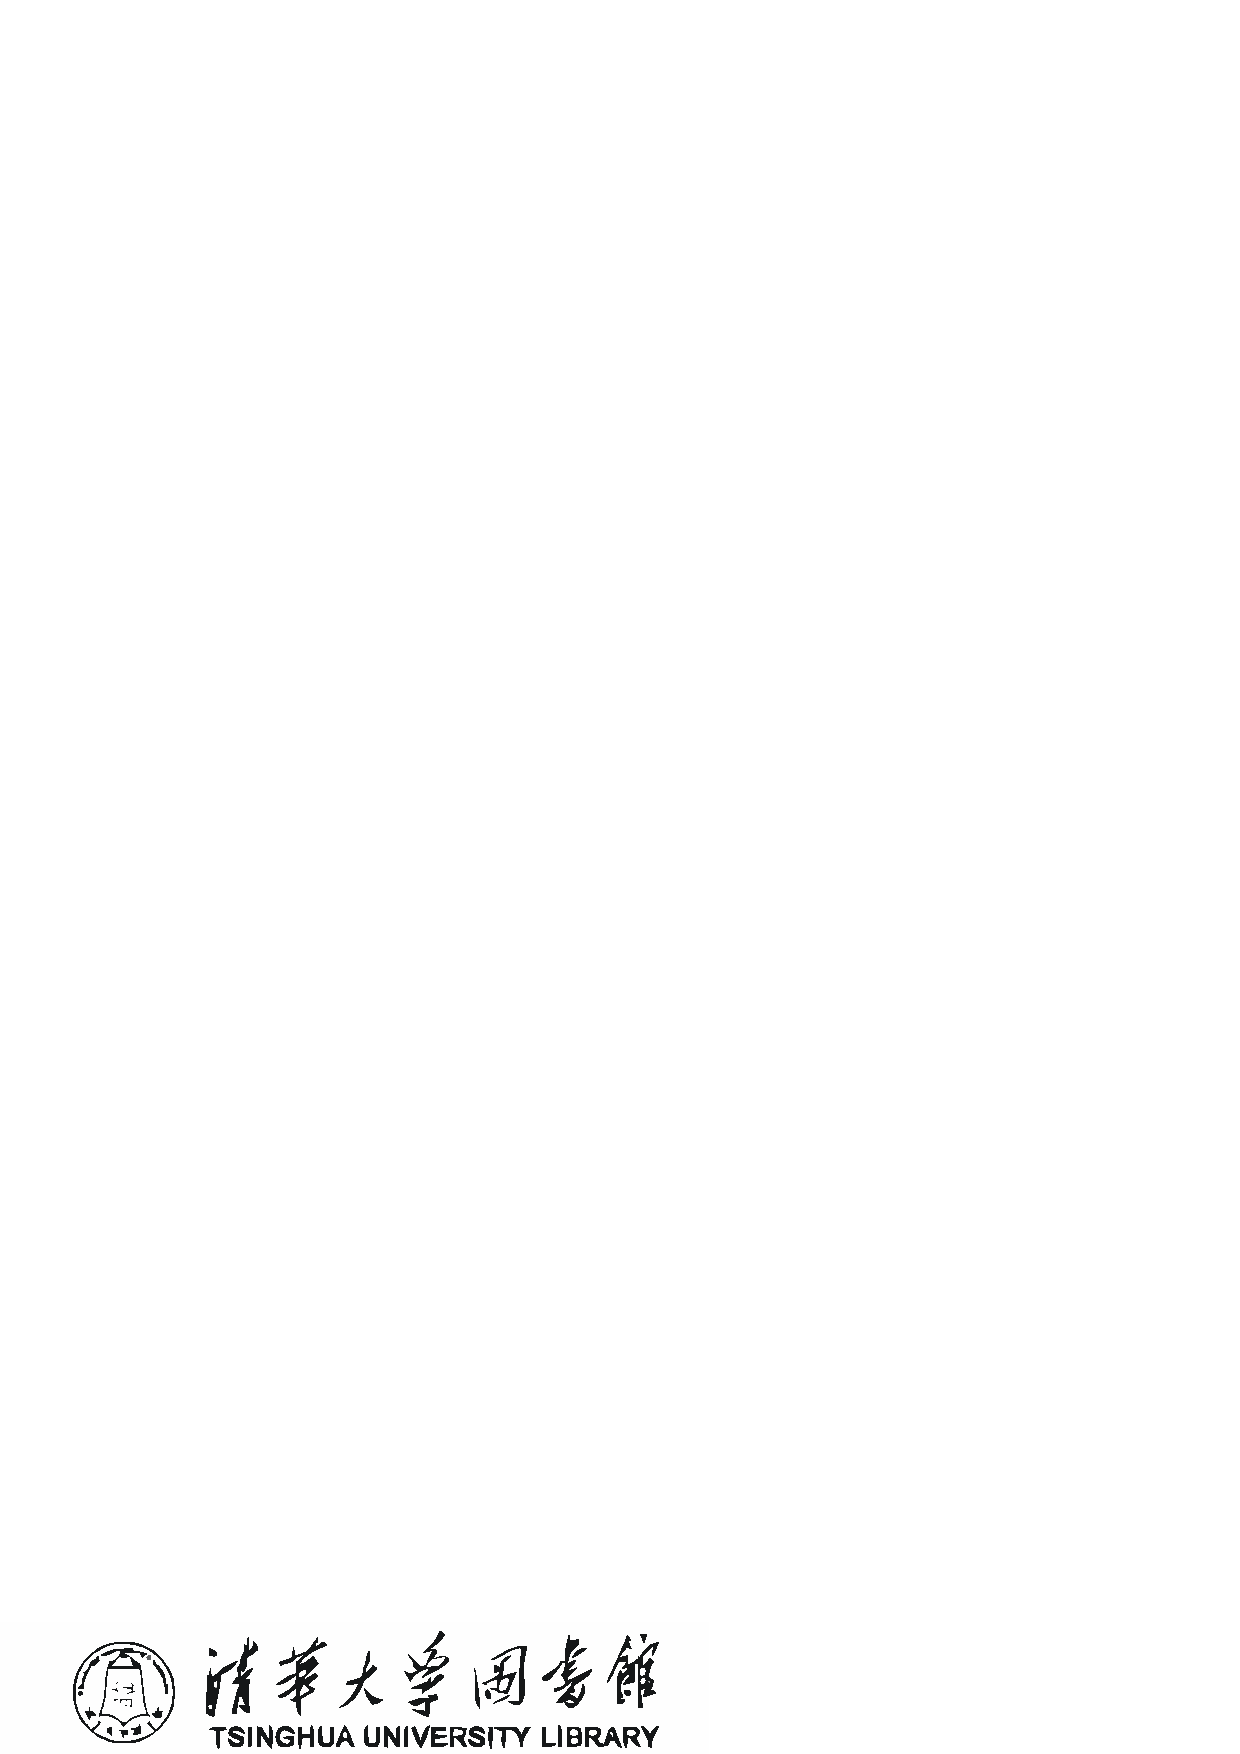
\includegraphics{thu-lib-logo}
  \caption*{Figure~1\quad This is an example for manually numbered figure,
    which would not appear in the list of figures}
  \label{tab:badfigure2}
\end{figure}

Now we consider a nonlinear programming which is confronted solely with
maximizing a real-valued function with domain $\Re^n$.  Whether derivatives are
available or not, the usual strategy is first to select a point in $\Re^n$ which
is thought to be the most likely place where the maximum exists. If there is no
information available on which to base such a selection, a point is chosen at
random. From this first point an attempt is made to construct a sequence of
points, each of which yields an improved objective function value over its
predecessor. The next point to be added to the sequence is chosen by analyzing
the behavior of the function at the previous points. This construction continues
until some termination criterion is met. Methods based upon this strategy are
called {\em ascent methods}, which can be classified as {\em direct methods},
{\em gradient methods}, and {\em Hessian methods} according to the information
about the behavior of objective function $f$. Direct methods require only that
the function can be evaluated at each point. Gradient methods require the
evaluation of first derivatives of $f$. Hessian methods require the evaluation
of second derivatives. In fact, there is no superior method for all
problems. The efficiency of a method is very much dependent upon the objective
function.

\subsection{Integer Programming}

{\em Integer programming} is a special mathematical programming in which all of
the variables are assumed to be only integer values. When there are not only
integer variables but also conventional continuous variables, we call it {\em
  mixed integer programming}. If all the variables are assumed either 0 or 1,
then the problem is termed a {\em zero-one programming}. Although integer
programming can be solved by an {\em exhaustive enumeration} theoretically, it
is impractical to solve realistically sized integer programming problems. The
most successful algorithm so far found to solve integer programming is called
the {\em branch-and-bound enumeration} developed by Balas (1965) and Dakin
(1965). The other technique to integer programming is the {\em cutting plane
  method} developed by Gomory (1959).

\hfill\textit{Uncertain Programming\/}\quad(\textsl{BaoDing Liu, 2006.2})

\section*{References}
\noindent{\itshape NOTE: These references are only for demonstration. They are
  not real citations in the original text.}

\begin{translationbib}
\item Donald E. Knuth. The \TeX book. Addison-Wesley, 1984. ISBN: 0-201-13448-9
\item Paul W. Abrahams, Karl Berry and Kathryn A. Hargreaves. \TeX\ for the
  Impatient. Addison-Wesley, 1990. ISBN: 0-201-51375-7
\item David Salomon. The advanced \TeX book.  New York : Springer, 1995. ISBN:0-387-94556-3
\end{translationbib}

\chapter{外文资料的调研阅读报告或书面翻译}

\title{英文资料的中文标题}

{\heiti 摘要:} 本章为外文资料翻译内容。如果有摘要可以直接写上来,这部分好像没有
明确的规定。

\section{单目标规划}
北冥有鱼,其名为鲲。鲲之大,不知其几千里也。化而为鸟,其名为鹏。鹏之背,不知其几
千里也。怒而飞,其翼若垂天之云。是鸟也,海运则将徙于南冥。南冥者,天池也。
\begin{equation}\tag*{(123)}
 p(y|\mathbf{x}) = \frac{p(\mathbf{x},y)}{p(\mathbf{x})}=
\frac{p(\mathbf{x}|y)p(y)}{p(\mathbf{x})}
\end{equation}

吾生也有涯,而知也无涯。以有涯随无涯,殆已!已而为知者,殆而已矣!为善无近名,为
恶无近刑,缘督以为经,可以保身,可以全生,可以养亲,可以尽年。

\subsection{线性规划}
庖丁为文惠君解牛,手之所触,肩之所倚,足之所履,膝之所倚,砉然响然,奏刀騞然,莫
不中音,合于桑林之舞,乃中经首之会。
\begin{table}[ht]
\centering
  \centering
  \caption*{表~1\hskip1em 这是手动编号但不出现在索引中的一个表格例子}
  \label{tab:badtabular3}
  \begin{tabular}[c]{|m{1.5cm}|c|c|c|c|c|c|}\hline
    \multicolumn{2}{|c|}{Network Topology} & \# of nodes &
    \multicolumn{3}{c|}{\# of clients} & Server \\\hline
    GT-ITM & Waxman Transit-Stub & 600 &
    \multirow{2}{2em}{2\%}&
    \multirow{2}{2em}{10\%}&
    \multirow{2}{2em}{50\%}&
    \multirow{2}{1.2in}{Max. Connectivity}\\\cline{1-3}
    \multicolumn{2}{|c|}{Inet-2.1} & 6000 & & & &\\\hline
    \multirow{2}{1.5cm}{Xue} & Rui  & Ni &\multicolumn{4}{c|}{\multirow{2}*{\thuthesis}}\\\cline{2-3}
    & \multicolumn{2}{c|}{ABCDEF} &\multicolumn{4}{c|}{} \\\hline
\end{tabular}
\end{table}

文惠君曰:“嘻,善哉!技盖至此乎?”庖丁释刀对曰:“臣之所好者道也,进乎技矣。始臣之
解牛之时,所见无非全牛者;三年之后,未尝见全牛也;方今之时,臣以神遇而不以目视,
官知止而神欲行。依乎天理,批大郤,导大窾,因其固然。技经肯綮之未尝,而况大坬乎!
良庖岁更刀,割也;族庖月更刀,折也;今臣之刀十九年矣,所解数千牛矣,而刀刃若新发
于硎。彼节者有间而刀刃者无厚,以无厚入有间,恢恢乎其于游刃必有余地矣。是以十九年
而刀刃若新发于硎。虽然,每至于族,吾见其难为,怵然为戒,视为止,行为迟,动刀甚微,
謋然已解,如土委地。提刀而立,为之而四顾,为之踌躇满志,善刀而藏之。”

文惠君曰:“善哉!吾闻庖丁之言,得养生焉。”


\subsection{非线性规划}
孔子与柳下季为友,柳下季之弟名曰盗跖。盗跖从卒九千人,横行天下,侵暴诸侯。穴室枢
户,驱人牛马,取人妇女。贪得忘亲,不顾父母兄弟,不祭先祖。所过之邑,大国守城,小
国入保,万民苦之。孔子谓柳下季曰:“夫为人父者,必能诏其子;为人兄者,必能教其弟。
若父不能诏其子,兄不能教其弟,则无贵父子兄弟之亲矣。今先生,世之才士也,弟为盗
跖,为天下害,而弗能教也,丘窃为先生羞之。丘请为先生往说之。”
\begin{figure}[h]
  \centering
  
\includegraphics{thu-whole-logo}
  \caption*{图~1\hskip1em 这是手动编号但不出现索引中的图片的例子}
  \label{tab:badfigure3}
\end{figure}

柳下季曰:“先生言为人父者必能诏其子,为人兄者必能教其弟,若子不听父之诏,弟不受
兄之教,虽今先生之辩,将奈之何哉?且跖之为人也,心如涌泉,意如飘风,强足以距敌,
辩足以饰非。顺其心则喜,逆其心则怒,易辱人以言。先生必无往。”

孔子不听,颜回为驭,子贡为右,往见盗跖。

\subsection{整数规划}
盗跖乃方休卒徒大山之阳,脍人肝而餔之。孔子下车而前,见谒者曰:“鲁人孔丘,闻将军
高义,敬再拜谒者。”谒者入通。盗跖闻之大怒,目如明星,发上指冠,曰:“此夫鲁国之
巧伪人孔丘非邪?为我告之:尔作言造语,妄称文、武,冠枝木之冠,带死牛之胁,多辞缪
说,不耕而食,不织而衣,摇唇鼓舌,擅生是非,以迷天下之主,使天下学士不反其本,妄
作孝弟,而侥幸于封侯富贵者也。子之罪大极重,疾走归!不然,我将以子肝益昼餔之膳。”


\chapter{其它附录}
前面两个附录主要是给本科生做例子。其它附录的内容可以放到这里,当然如果你愿意,可
以把这部分也放到独立的文件中,然后将其 \cs{input} 到主文件中。

    \end{appendix}
    
    %% 个人简历
    \begin{resume}

  \resumeitem{个人简历}

  xxxx 年 xx 月 xx 日出生于 xx 省 xx 县。

  xxxx 年 9 月考入 xx 大学 xx 系 xx 专业,xxxx 年 7 月本科毕业并获得 xx 学士学位。

  xxxx 年 9 月免试进入 xx 大学 xx 系攻读 xx 学位至今。

  \researchitem{发表的学术论文} % 发表的和录用的合在一起

  % 1. 已经刊载的学术论文(本人是第一作者,或者导师为第一作者本人是第二作者)
  \begin{publications}
    \item Yang Y, Ren T L, Zhang L T, et al. Miniature microphone with silicon-
      based ferroelectric thin films. Integrated Ferroelectrics, 2003,
      52:229-235. (SCI 收录, 检索号:758FZ.)
    \item 杨轶, 张宁欣, 任天令, 等. 硅基铁电微声学器件中薄膜残余应力的研究. 中国机
      械工程, 2005, 16(14):1289-1291. (EI 收录, 检索号:0534931 2907.)
    \item 杨轶, 张宁欣, 任天令, 等. 集成铁电器件中的关键工艺研究. 仪器仪表学报,
      2003, 24(S4):192-193. (EI 源刊.)
  \end{publications}

  % 2. 尚未刊载,但已经接到正式录用函的学术论文(本人为第一作者,或者
  %    导师为第一作者本人是第二作者)。
  \begin{publications}[before=\publicationskip,after=\publicationskip]
    \item Yang Y, Ren T L, Zhu Y P, et al. PMUTs for handwriting recognition. In
      press. (已被 Integrated Ferroelectrics 录用. SCI 源刊.)
  \end{publications}

  % 3. 其他学术论文。可列出除上述两种情况以外的其他学术论文,但必须是
  %    已经刊载或者收到正式录用函的论文。
  \begin{publications}
    \item Wu X M, Yang Y, Cai J, et al. Measurements of ferroelectric MEMS
      microphones. Integrated Ferroelectrics, 2005, 69:417-429. (SCI 收录, 检索号
      :896KM)
    \item 贾泽, 杨轶, 陈兢, 等. 用于压电和电容微麦克风的体硅腐蚀相关研究. 压电与声
      光, 2006, 28(1):117-119. (EI 收录, 检索号:06129773469)
    \item 伍晓明, 杨轶, 张宁欣, 等. 基于MEMS技术的集成铁电硅微麦克风. 中国集成电路,
      2003, 53:59-61.
  \end{publications}

  \researchitem{研究成果} % 有就写,没有就删除
  \begin{achievements}
    \item 任天令, 杨轶, 朱一平, 等. 硅基铁电微声学传感器畴极化区域控制和电极连接的
      方法: 中国, CN1602118A. (中国专利公开号)
    \item Ren T L, Yang Y, Zhu Y P, et al. Piezoelectric micro acoustic sensor
      based on ferroelectric materials: USA, No.11/215, 102. (美国发明专利申请号)
  \end{achievements}

\end{resume}

    
    %% 本科生进行格式审查是需要下面这个表格,答辩可能不需要。选择性留下。
    % 综合论文训练记录表
    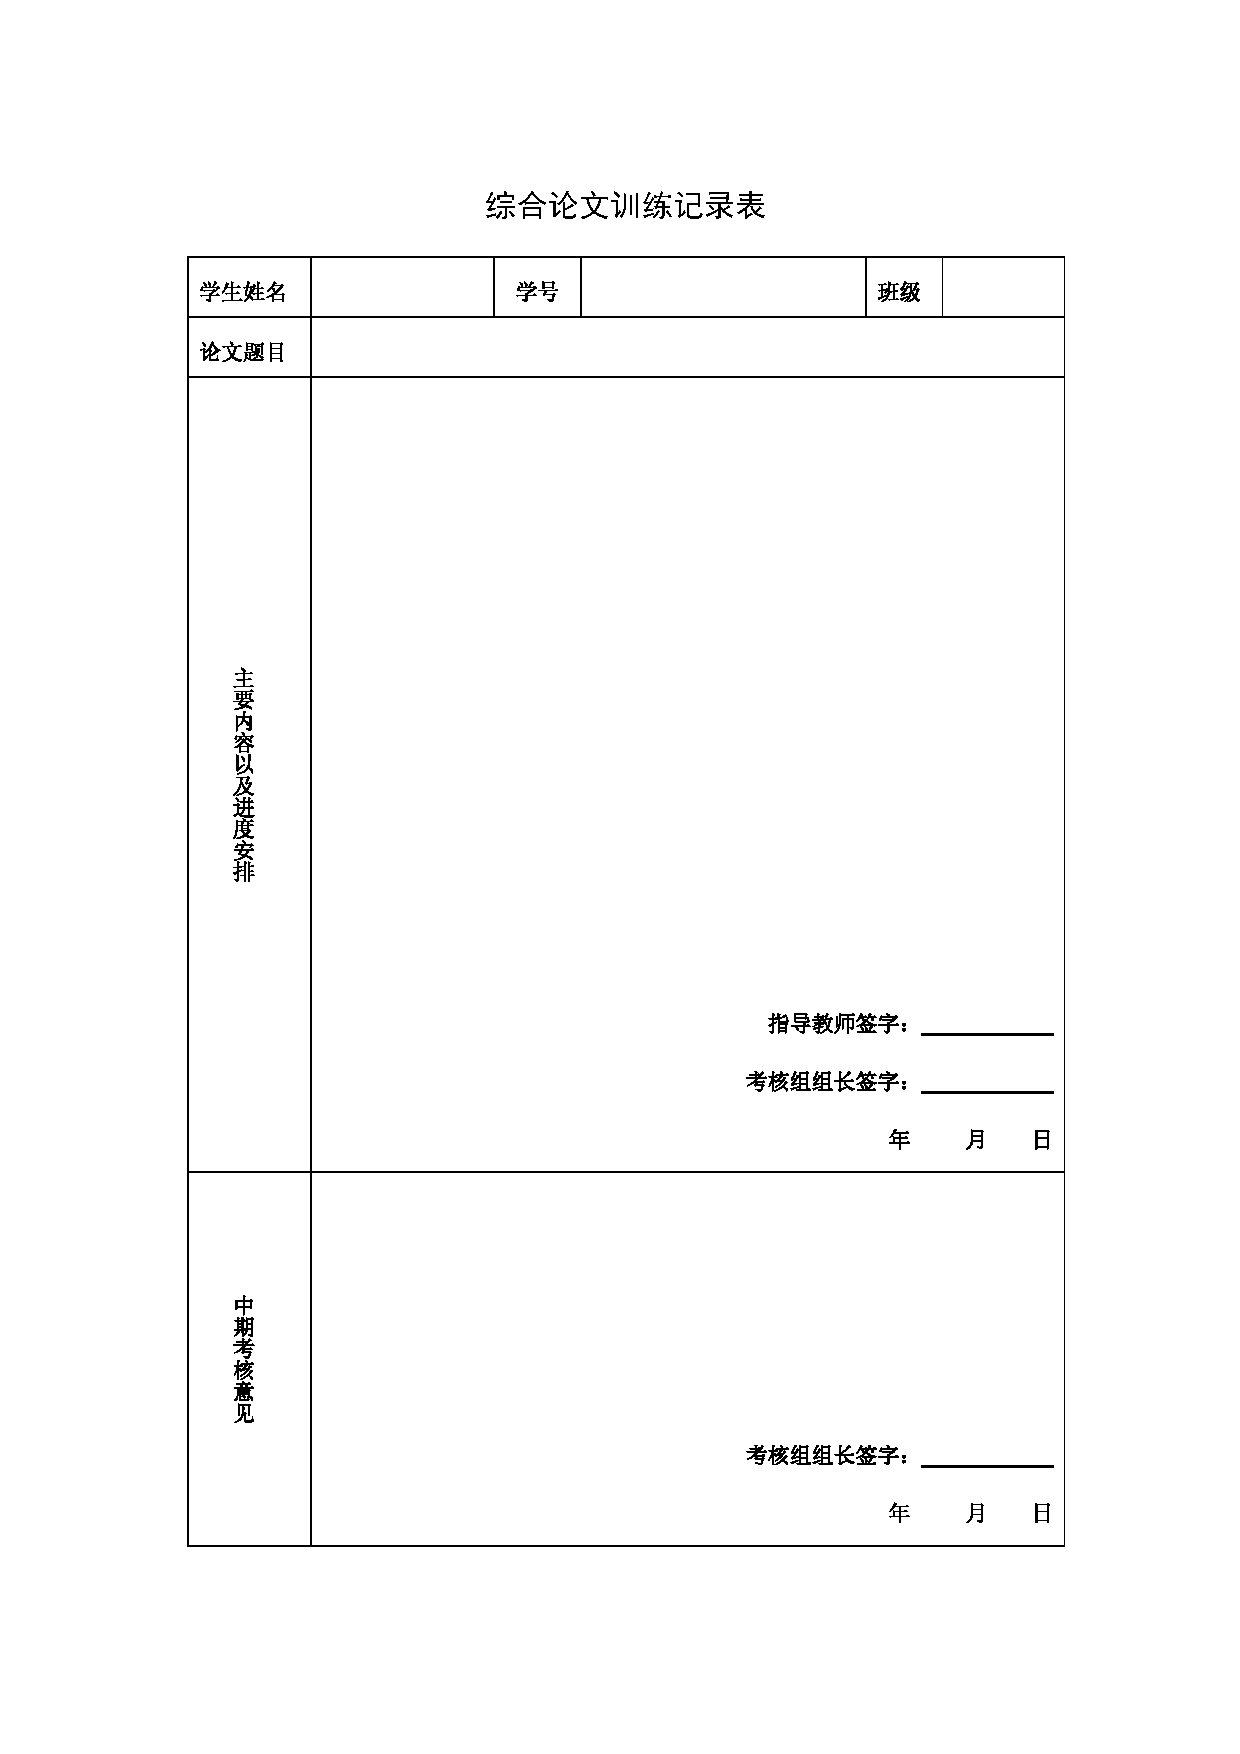
\includepdf[pages=-]{scan-record.pdf}
    \end{document}
    